% %%%%%%%%%%%%%%%%%%%%%%%%%%%%%%%%%%%%%%%%%%%%%%%%%%%%%%%%%%%%%%%%%%%%%%% %
%                                                                         %
% The Project Gutenberg EBook of Transactions of the American Society of  %
% Civil Engineers, vol. LXX, Dec. 1910, by Ralph C. Taggart               %
%                                                                         %
% This eBook is for the use of anyone anywhere at no cost and with        %
% almost no restrictions whatsoever.  You may copy it, give it away or    %
% re-use it under the terms of the Project Gutenberg License included     %
% with this eBook or online at www.gutenberg.org                          %
%                                                                         %
%                                                                         %
% Title: Transactions of the American Society of Civil Engineers, vol. LXX, Dec. 1910
%        Expansion of Pipes, Paper No. 1167                               %
%                                                                         %
% Author: Ralph C. Taggart                                                %
%                                                                         %
% Release Date: April 28, 2008 [EBook #25220]                             %
%                                                                         %
% Language: English                                                       %
%                                                                         %
% Character set encoding: ISO-8859-1                                      %
%                                                                         %
% *** START OF THIS PROJECT GUTENBERG EBOOK SOCIETY OF CIVIL ENGINEERS ***%
%                                                                         %
% %%%%%%%%%%%%%%%%%%%%%%%%%%%%%%%%%%%%%%%%%%%%%%%%%%%%%%%%%%%%%%%%%%%%%%% %

\def\ebook{25220}
\newtoks\PGheader
{\catcode`\#11\relax\catcode`\L\active\obeylines\obeyspaces%
\global\PGheader={%
The Project Gutenberg EBook of Transactions of the American Society of
Civil Engineers, vol. LXX, Dec. 1910, by Ralph C. Taggart

This eBook is for the use of anyone anywhere at no cost and with
almost no restrictions whatsoever.  You may copy it, give it away or
re-use it under the terms of the Project Gutenberg License included
with this eBook or online at www.gutenberg.org


Title: Transactions of the American Society of Civil Engineers, vol. LXX, Dec. 1910
       Expansion of Pipes, Paper No. 1167

Author: Ralph C. Taggart

Release Date: April 28, 2008 [EBook #25220]

Language: English

Character set encoding: ISO-8859-1

*** START OF THIS PROJECT GUTENBERG EBOOK SOCIETY OF CIVIL ENGINEERS ***
}}
\AtBeginDocument{\CreditsLine{%
Produced by Juliet Sutherland, David Wilson and the Online
Distributed Proofreading Team at http://www.pgdp.net
}}

%%%%%%%%%%%%%%%%%%%%%%%%%%%%%%%%%%%%%%%%%%%%%%%%%%%%%%%%%%%%%%%%%%%%%%%%%%%
%%                                                                       %%
%% Packages and substitutions:                                           %%
%%                                                                       %%
%% memoir:   Advanced book class. Required.                              %%
%% memhfixc: Part of memoir; needed to work with hyperref. Required.     %%
%% amsmath:  AMS mathematics enhancements. Required.                     %%
%% amssymb:  extra AMS mathematics symbols. Required.                    %%
%% hyperref: Hypertext embellishments for pdf output. Required.          %%
%%           Driver option needs to be set explicitly.                   %%
%% graphicx: standard graphics inclusion package. Required.              %%
%%           Driver option needs to be set explicitly.                   %%
%% wrapfig:  Allows placement of graphics inside text cutouts. Required. %%
%% flafter:  Stops graphics floating backwards. Required.                %%
%% perpage:  Resets footnote markers every page. Optional.               %%
%%                                                                       %%
%%                                                                       %%
%% Producer's Comments: No great dramas with formatting the mathematics. %%
%%           Too many pagination-dependent manual tweaks. Deciphering    %%
%%           the functions plotted in figures 23-25 was an effort: see   %%
%%           comments at 013.png below.                                  %%
%%                                                                       %%
%% Things to Check:                                                      %%
%%                                                                       %%
%% hyperref and graphicx driver option matches workflow: OK              %%
%% color driver option matches workflow (color package is called         %%
%%    by hyperref, so may rely on color.cfg): OK                         %%
%% graphicx driver can handle PNG and PDF graphics: OK                   %%
%% fonts: assumes text and math numerals are drawn from the same font    %%
%% Spellcheck: OK                                                        %%
%% Smoothreading pool: No                                                %%
%% LaCheck: OK                                                           %%
%% Lprep/gutcheck: OK                                                    %%
%% PDF pages: 47                                                         %%
%% PDF page size: 499 x 709pt (b5)                                       %%
%% PDF document info: filled in                                          %%
%% PDF bookmarks: none generated                                         %%
%% marginal notes in "Discussion" at end correct for each pagebreak      %%
%% text cutouts around wrapped graphics not crossing page breaks--       %%
%%    Figs 1 on p4, 26 on p27, 27 on p29, 28 on p32, 29 on p33           %%
%% no overfull boxes; two underfull hboxes                               %%
%%                                                                       %%
%% Compile sequence:                                                     %%
%%                                                                       %%
%% pdflatex x3                                                           %%
%%                                                                       %%
%% Compile history:                                                      %%
%%                                                                       %%
%% April 08: dcwilson.                                                   %%
%%           Compiled with pdfLaTeX THREE times.                         %%
%%           MiKTeX 2.7, Windows XP Pro                                  %%
%%                                                                       %%
%%                                                                       %%
%%%%%%%%%%%%%%%%%%%%%%%%%%%%%%%%%%%%%%%%%%%%%%%%%%%%%%%%%%%%%%%%%%%%%%%%%%%

\listfiles

\makeatletter

\documentclass[b5paper,12pt,twoside,openany,onecolumn]{memoir}[2005/09/25]

\setlrmarginsandblock{2.3cm}{2.6cm}{*}
\setulmarginsandblock{3.1cm}{2.2cm}{*}
\setlength{\headsep}{1cm}
\setlength{\footskip}{0.6cm}
\fixthelayout
\typeoutlayout
%
% font issues
% Courier, for the PG licence stuff
\DeclareRobustCommand\ttfamily % Courier, for the PG licence stuff
        {\not@math@alphabet\ttfamily\mathtt
         \fontfamily{pcr}\fontencoding{T1}\selectfont}

\IfFileExists{lmodern.sty}
{% use the mathcomp symbol for degrees (we don't want to load the whole package though)
 \GenericInfo{*** }{*** Using Latin Modern for degree symbol...\@gobble}
 \@namedef{TS1:lmr}{0}
 \input{ts1enc.def}
 \DeclareSymbolFont{TC}{TS1}{lmr}{m}{n}
 \DeclareMathSymbol{\tcdegree}{\mathord}{TC}{176}
 \let\degrees\tcdegree
}{% else just use the less authentic ^\circ
 \def\degrees{^\circ}
}

% mathematics
\usepackage[reqno]{amsmath}[2000/07/18]
\usepackage[psamsfonts]{amssymb}[2002/01/22]
\DeclareMathOperator{\Sin}{sin\kern-0.1em.}
\DeclareMathOperator{\Cos}{cos\kern-0.1em.}
\DeclareMathOperator{\Tan}{tan\kern-0.1em.}

% footnotes
\newfootnoteseries{T} % for transcriber's notes
\plainfootstyle{T}
\renewcommand{\thefootnote}{\BringhurstX{footnote}}
\footmarkstyle{#1\hfill}
\footmarkstyleT{#1.\hfill}
\renewcommand{\foottextfont}{\footnotesize\normalfont}
\let\foottextfontT\foottextfont
\setlength{\footmarksep}{\z@}
\setlength{\footmarkwidth}{1.3em}
\IfFileExists {perpage.sty}
{% use the installed version
 \usepackage{perpage}[2002/12/20]}{% else load the guts of an old David Kastrup version (LPPL)
 \newcommand*\MakePerPage[2][\@ne]{%
  \expandafter\def\csname c@pchk@##2\endcsname{\c@pchk@{##2}{##1}}%
  \newcounter{pcabs@##2}%
  \@addtoreset{pchk@##2}{##2}}
 \def\new@pagectr##1{\@newl@bel{pchk@##1}}
 \def\c@pchk@##1##2{\z@=\z@
  \begingroup
  \expandafter\let\expandafter\next\csname pchk@##1@\arabic{pcabs@##1}\endcsname
  \addtocounter{pcabs@##1}\@ne
  \expandafter\ifx\csname pchk@##1@\arabic{pcabs@##1}\endcsname\next
  \else \setcounter{##1}{##2}\fi
  \protected@edef\next{%
    \string\new@pagectr{##1}{\arabic{pcabs@##1}}{\noexpand\thepage}}%
  \protected@write\@auxout{}{\next}%
  \endgroup\global\z@}
}
\MakePerPage{footnote}
\def\BringhurstX#1{\expandafter\@BringhurstX\csname c@#1\endcsname}
\def\@BringhurstX#1{\ifcase#1\or*\or\dag\or\ddag\or\S\or$\|$\or\P
  \or**\or\dag\dag\or\ddag\ddag\or\S\S\or$\|\|$\or\P\P\else?\fi}

% illustrations
% (external files are either .png or .pdf)
\usepackage{flafter}[2000/07/23]
% defaults are not stretchy enough
\setlength\textfloatsep{20\p@ \@plus 6\p@ \@minus 4\p@}
\setlength\intextsep   {14\p@ \@plus 8\p@ \@minus 4\p@}
\renewcommand\floatpagefraction{0.5}
\newcommand\Legend[1]{\legend{Fig.\ #1.}\DPanchor{fig:#1}\vskip-14pt}
\newcommand\figref[1]{\hyperlink{fig:#1}{Fig.~#1}}
% driver should be specified in graphics.cfg;
% if not, add explicit option to graphicx call
\usepackage[final]{graphicx}[1999/02/16]
\GenericWarning{*** }{***\MessageBreak
 Important Note: this document comes with PNG and PDF\MessageBreak
 graphics, so make sure you use an appropriate workflow!\MessageBreak
 \expandafter\@gobble\@gobble}
\RequirePackage{wrapfig}[2003/01/31]
\captionstyle{\centering}
\captiontitlefont{\normalfont\Small\scshape}

% PDF stuff: links, document info, etc
% if default driver given in hyperref.cfg is not suitable,
% add appropriate explicit option to hyperref call
\usepackage[final,colorlinks]{hyperref}[2003/11/30]
% we check if the driver is the useless (for pdf) "hypertex",
% and if so we force pdftex instead and issue a warning
\def\@tempa{hypertex}
\ifx\@tempa\Hy@defaultdriver
  \GenericWarning{*** }{***\MessageBreak
   Inappropriate driver for hyperref specified: assuming pdftex.\MessageBreak
   You should amend the source code if using another driver.\MessageBreak
   \expandafter\@gobble\@gobble}
  \Hy@SetCatcodes\input{hpdftex.def}\Hy@RestoreCatcodes
\fi
\usepackage{memhfixc}[2004/05/13]
\providecommand\ebook{2wxyz}
\hypersetup{pdftitle=The Project Gutenberg eBook \#\ebook: Expansion of Pipes,
  pdfsubject=American Society of Civil Engineers - Transactions - Paper 1167,
  pdfauthor=Ralph C. Taggart,
  pdfkeywords={Juliet Sutherland, David Wilson,
               Project Gutenberg Online Distributed Proofreading Team},
  pdfstartview=Fit,
  pdfstartpage=1,
  pdfpagemode=UseNone,
  pdfdisplaydoctitle,
  bookmarksopen,
  bookmarksopenlevel=1,
  linktocpage=false,
  pdfpagescrop=0 0 499 709, b5paper, % b5 176x250mm
  pdfpagelayout=TwoPageRight, % this is Acrobat 6's "Facing"
  plainpages=false, linkcolor=\ifdraftdoc blue\else black\fi,
  menucolor=\ifdraftdoc blue\else black\fi,
  citecolor=\ifdraftdoc blue\else black\fi,
  urlcolor=\ifdraftdoc magenta\else black\fi}

% for adding explicit destinations
\newcommand\DPanchor[1]{\rlap{\hyper@anchorstart{#1}\hyper@anchorend}}
\def\Tag#1{\DPanchor{eq:#1}\tag{#1}}

% A quasi-verbatim environment for boilerplate, slightly less drastic than alltt
% Spaces, linebreaks, $ , % and # will appear as typed
% but unlike full verbatim, commands will still be interpreted and long lines will wrap
% (comments documenting the boilerplate text need to use | as the comment character)
% uses slightly non-standard obeylines and active space.
% The optional argument can be used to specify an explicit font size for the boilerplate.
% If no optional argument is provided, a fontsize will be computed to allow--as nearly as
% possible--73 fixed-width characters per \textwidth (the longest line in the PG license
% has 73 characters)
{\catcode`\^^M=\active % these lines must end with %
  \global\def\PGobeylines{\catcode`\^^M\active \def^^M{\null\par}}}%
{\obeyspaces%
\global\def\PGb@ilerplate[#1]{\def\PGb@ilerplateHook{#1}\catcode`\%11\relax%
\catcode`\$11\relax\catcode`\#11\relax\catcode`\|=14\relax%
\pretolerance=\@m\hyphenpenalty=5000%
\rightskip=\z@\@plus20em\relax%
\frenchspacing\ttfamily\PGb@ilerplateHook%
\def {\noindent\null\space}%
\parindent=\z@\PGobeylines\obeyspaces}}
\def\PGboilerplate{%
 \@ifnextchar[{\PGb@ilerplate}{\PGb@ilerplate[\PGAutoFit{73}]}}
\let\endPGboilerplate\empty
% \PGAutoFit adjusts the fontsize so a specified number of
% fixed-width characters will fit in the current \textwidth
\def\PGrem@pt#1.#2Q@!!@Q{#1}
\def\PGAutoFit#1{\setbox\z@=\hbox{m}\dimen@=\wd\z@\relax
  \multiply\dimen@#1\relax \dimen@i=\dimen@\relax
  \dimen@=\textwidth\relax
  \dimen@ii=\f@size pt  \advance\dimen@ii0.5pt
  \expandafter\multiply\expandafter\dimen@\expandafter\PGrem@pt\the\dimen@ii Q@!!@Q
  \expandafter\divide\expandafter\dimen@\expandafter\PGrem@pt\the\dimen@i Q@!!@Q
  \dimen@i=\dimen@\multiply\dimen@i12\divide\dimen@i10
  \fontsize{\strip@pt\dimen@}{\strip@pt\dimen@i}\ttfamily\selectfont}
{\catcode`\L\active
\gdef\PGlicencelink{\catcode`\L\active\letL\PGlinklicence}}
\def\PGlinklicence{\@ifnextchar i{\PG@lli}{L}}
\def\PG@lli#1{\@ifnextchar c{\PG@llii}{Li}}
\def\PG@llii#1{\@ifnextchar e{\PG@lliii}{Lic}}
\def\PG@lliii#1{\@ifnextchar n{\PG@lliv}{Lice}}
\def\PG@lliv#1{\@ifnextchar s{\PG@llv}{Licen}}
\def\PG@llv#1{\@ifnextchar e{\PG@llvi}{Licens}}
\def\PG@llvi#1{\hyperlink{PGlicence}{License}}

% half-title and copyright pages
\let\transcribersnotes\@empty
\let\transcribersNotes\@empty
\newcommand{\transcribersnote}[1]{%
  \@ifnotempty{#1}{\g@addto@macro\transcribersnotes{#1\par}%
    \@xp\@ifempty\@xp{\transcribersNotes}%
      {\renewcommand{\transcribersNotes}{Transcriber's note}}
      {\renewcommand{\transcribersNotes}{Transcriber's notes}}}}
\newcommand{\CreditsLine}[1]{\newcommand{\thePr@ductionTeam}{#1}}

\def\makehalftitlepage{% the boilerplate header
  \begingroup
  \pagestyle{empty}
  \pagenumbering{Alph} % to ensure unique hyperref page anchors
  \begin{PGboilerplate}[\tiny] % 8pt for B5
    \PGlicencelink
    \the\PGheader
  \end{PGboilerplate}
  \null\vfil
  \clearpage
  \endgroup}

\def\makecopyrightpage{% production credits and transcriber's notes
  \begingroup\pagestyle{empty}
  \null\vfil
  \begin{center}
    \thePr@ductionTeam
  \end{center}
  \vfil\vfil
  \vbox{\Small\hsize=.75\textwidth\parindent=\z@\parskip=.75em
  \textit{\transcribersNotes}\par\medskip\raggedright
  \transcribersnotes\par}
  \cleartorecto
  \endgroup}

% headers and footers
\copypagestyle{mainstuff}{headings}
\makepsmarks{mainstuff}{%
      \let\@mkboth\markboth
      \def\chaptermark##1{%
        \markboth{\MakeUppercase{##1}}{\MakeUppercase{##1}}}%
    }
\makeevenhead{mainstuff}{\normalfont\SMALL\thepage}{\normalfont
    \SMALL\MakeUppercase{\leftmark}}{}
\makeoddhead{mainstuff}{}{\normalfont
    \SMALL\MakeUppercase{\rightmark}}{\normalfont\SMALL\thepage}
\pagestyle{mainstuff}

\copypagestyle{licence}{headings}
\makeevenhead
  {licence}{\normalfont\SMALL\thepage}{\normalfont\SMALL LICENSING}{}
\makeoddhead
  {licence}{}{\normalfont\SMALL LICENSING}{\normalfont\SMALL\thepage}

% for the sidenotes in the Discussion
% these need to be placed manually at the top of each page where a
% speaker's contribution carries across a pagebreak
%
\def\speaker#1{\marginpar{\centering\tiny\noindent#1}}

% to deal with the scanned page breaks
% add a "draft" option to the documentclass invocation
% to see the scan numbers
\ifdraftdoc
\def\PG#1 #2.png#3
{\marginpar{\noindent\null\hfill\Small #2.png}}
\def\PGx#1 #2.png#3
{}
\else
\def\PG#1 #2.png#3
{}
\let\PGx\PG
\fi


% bits and pieces
\emergencystretch=12pt
\setlength\parskip{0\p@ \@plus 3\p@}
\let\Small\footnotesize
\let\SMALL\scriptsize
\def\verybigskip{\vskip14pt plus8pt minus4pt}


\makeatother

\begin{document}

\makehalftitlepage

\transcribersnote{This paper was originally published in volume LXX, December 1910.}

\transcribersnote{Author footnotes are labelled using printer's
 marks\footnotemark; footnotes showing where corrections to the text
 have been made are labelled numerically\footnotemarkT.}

\transcribersnote{\SMALL Minor typographical corrections are documented in the \LaTeX\ source.}

\makecopyrightpage

\mainmatter\setcounter{footnoteT}{0}
\PG--File: 001.png---\*********\*****\************\*********\--------------




\begin{center}
{\Large AMERICAN SOCIETY OF CIVIL ENGINEERS}\\
{\tiny I\;N\;S\;T\;I\;T\;U\;T\;E\;D\;~\;1\;8\;5\;2}\\
 \rule[3pt]{.2\textwidth}{.4pt} \\[6pt]
\textbf{\LARGE TRANSACTIONS}\\
 \rule[3pt]{.1\textwidth}{.4pt} \\
\textbf{\small Paper No.~1167}\\
 \rule[3pt]{.2\textwidth}{.4pt} \\[3pt]
{\large EXPANSION OF PIPES.} \\
\smallskip
\textsc{By Ralph C. Taggart, Assoc.\ M. Am.\ Soc.\ C.\ E.}\\
\rule[3pt]{.2\textwidth}{.4pt} \\
\textsc{\small With Discussion by Messrs. William D.~Ennis, William Kent,\\
 and Ralph C.~Taggart.}\\
\rule[3pt]{.2\textwidth}{.4pt}
\end{center}\chaptermark{Expansion of Pipes}\thispagestyle{empty}
\bigskip

In the arrangement of steam piping (or other piping, the temperature
of which is subject to considerable change), proper allowance must
be made for expansion. Where the change in temperature, and hence
the amount of expansion, is small, the stress may come well within the
elastic limit of the metal. In such cases, of course, special arrangements
to care for the expansion may not be required.

The calculation to determine the allowable stress in pipe may be
readily made. In the case of ordinary iron pipe, we have the
following:

The modulus of elasticity of wrought iron, or the stress divided
by the strain, equals 29\,000\,000.

The coefficient of expansion of wrought iron, or the increase in
length per degree Fahrenheit per unit length, is 0.00000673.

The stress per degree Fahrenheit, therefore, would be 29\,000\,000
times 0.00000673, which is equal to 195.2~lb.\ per sq.\ in.\ per degree
Fahrenheit difference in temperature. For a change in temperature
of $100\degrees$~Fahr., the stress would become 19\,520~lb.\ per sq.\ in., which
is more than the safe working stress in the iron, especially when
it is considered that the stress would be largely increased at the
various screw joints, where the thickness of the pipe is reduced by the
depth of the thread.
\PG--File: 002.png---\*********\******\************\*******\---------------

For ordinary steam apparatus the change in temperature is at
least $150\degrees$~Fahr., so that it becomes impossible for the elasticity of
the metal to care for the expansion, even if the piping is very securely
tied down. For, when the elastic limit of the metal is reached, a
permanent set will result, and if this change in the form of the piping
is repeated, a rupture may be expected.

In steam piping, expansion is cared for by two general methods:
First, by the use of so-called expansion joints; and second, by the
arrangement of the piping, so that the expansion is cared for by the
spring of the piping itself.

In apparatus where the straight runs of pipe have not been too
long, the second method has been used almost exclusively, although
the allowance for expansion has usually been one of judgment or guesswork,
and not a matter of calculation.

Where the expansion has been considerable at any one place, it
has been common practice for the designing engineer to resort to the
use of so-called expansion joints. There are numerous types of these
joints, and although many of them have merit, the writer believes
that, for many purposes, there are objections to all types. One of the
best-known types is made with one metal cylinder sliding or slipping
within another. There is, ordinarily, a packed gland or stuffing-box
to prevent leakage. An expansion joint of this type should always be
anchored, and the pipe which moves within it should also be anchored
at a point some distance from it---the distance being determined by
the amount of expansion which this particular joint should care for.
If the pipe and expansion joint are not thus anchored, the movement
of the pipe and the thrust of the steam pressure may carry the inner
cylinder of the expansion joint entirely away from the outer cylinder
in which it moves. This type requires more or less packing, and although
this may not be an important item if only a few expansion
joints are used, and if they can be gotten at readily, nevertheless it
becomes very important where an engineer has to look after a number
of these joints, or where they cannot be reached with the greatest ease.

In a second type of expansion joint, a circular metal disk is fixed at
its outer circumference and attached to the expanding pipe near its
center. The expansion is taken care of by the spring in the metal
disk, and, for this reason, the amount is usually quite small.
\PG--File: 003.png---\*********\******\*********\*******\------------------

A third type of expansion joint is made up of what may be described
as a copper pipe with deep corrugations, reinforced with steel rings.
Under certain conditions this joint has been very unsatisfactory.
Where it has been subjected to varying temperatures, as, for example,
in a heating apparatus where the steam pressure is more or less intermittent,
the movement in the copper has resulted in breaking at the
corrugations. It is claimed, however, that some good results have been
obtained where the steam pressure was not very high, and where the
pressure and temperature have been very constant.

Some authorities have suggested the use of fittings arranged so
that the expansion will be cared for by the twisting of the pipe within
the thread of the fitting. This has been done in some cases in low-pressure
work, but a little thought or experience will convince one
that it is not a method to be relied on, for as soon as the slightest
actual twist occurs within the fitting, the pipe becomes loose, and the
joint formed by any white lead or varnish is broken. This destroys
the effect of the white lead or varnish, and the difficulty of making an
ordinary pipe joint tight without some such cement is well known.
In many cases, where it is thought that the expansion is cared for
by a twisting in a fitting, a careful examination will show that it is
really cared for entirely by the spring of the pipe, and it may be set
down as a safe rule that, if there is actually a twist in the pipe-thread,
due to expansion, there will almost surely be a leak, even where the
pressures are low.

It may be interesting, here, to mention what is known as water
packing. A so-called steam-tight joint is sometimes made where one
piece of metal slips within another, a few circular rings or grooves
being cut in one of the cylinders. The fit, of course, must be very
good, and the idea is that the condensed steam in the rings or grooves
forms a sort of packing. This arrangement is used with engine indicators
and with some reducing-pressure valves of the piston type, where
a steam-tight joint is desired and where one cylinder must slip within
the other. The success of the joint depends on two things: First, and
principally, on very accurate workmanship; and second, on the fact
that if a very little steam passes through the joint, any part of it
which is condensed will evaporate immediately and pass away unnoticed.
This is very soon proven, if the discharge from a reducing-pressure
valve of this type is closed, and the line leading to it fills with
\PG--File: 004.png---\*********\******\*********\********\-----------------
water, when it will be seen that water is leaking from the joint. This
is one reason for the old saying that it is easier to make a joint steam-tight
than water-tight.

The most common way in which expansion is cared for in steam
piping is by the spring or bending of the pipes, where a change in
direction occurs, and, on the whole, this method is the most satisfactory.
The allowance to be made for expansion, or the length of the
spring pieces, however, is usually guessed at, or is determined by
experience, rather than by accurate calculation.

Some years ago, the writer made calculations of the lengths of
spring pieces for a large underground installation, and, from these
calculations, he made a number of diagrams, which he has used to a
considerable extent since that time. More recently, however, the
\begin{wrapfigure}{r}{.5\textwidth}
 \includegraphics[width=.5\textwidth]{images/illus-004}
 \Legend{1}
\end{wrapfigure}
original calculations have been
somewhat extended, and this paper
contains the resulting diagrams
and curves, both new and old,
together with a short explanation
of their derivation and use. It
is believed that they will be of
value to designing engineers and
others.

\figref{1} represents two lengths
of pipe, $l_1$ and $l_2$, connected by a
$90\degrees$ elbow. The lengths, $l_1$ and $l_2$,
are supposed to represent the
distances from the elbow to the points at which the pipe is held in
line, or at which the pipe, if horizontal or vertical before expansion,
must remain horizontal or vertical after expansion. It will be assumed
that the principal expansion acts in a direction at right angles to $l_1$
and that the secondary or smaller relative expansion, if any, acts at
right angles to $l_2$. Consider, first, a condition in which the secondary
expansion is zero. The expansion is then at right angles to $l_1$ and
while the spring in the length of pipe, $l_1$ must care largely for the
expansion, the length, $l_2$, is also a determining factor. If $l_2$ becomes
zero, or if the pipe at both ends of the length, $l_1$ is held horizontally,
it is easy to determine the length of $l_1$ required for any given expansion,
when the size of the pipe is known.
\PG--File: 005.png---\*********\******\*********\********\-----------------

Under these conditions the formula may be worked out, and will
be found to be as follows:
\[
{l_1}^2 =  \dfrac{87\,000\,000\; Dr}{f}             \Tag{1}
\]
where the modulus of elasticity is taken as that of wrought iron or
steel, \emph{viz.}, 29\,000\,000.
\begin{flalign*}
\rlap{\indent Where}&& l_1 &= \text{the length of pipe under strain, in inches;}\\
          && r &= \text{the expansion, in inches, at right angles to the length}\\
          &&&\qquad\text{of pipe, $l_1$;}\\
          && D &= \text{the outside diameter of pipe, in inches; and,}\\
          && f &= \text{the maximum fiber stress, in pounds per square inch.}
\end{flalign*}

This does not allow for the weakening of the pipe at the fitting.

In the case under consideration, the maximum strain occurs at
both ends of the length, $l_1$ of the pipe, and therefore the lessening in
strength at the elbow or fitting should be considered, and allowance
made therefor. For example, if the pipe is weaker than the fitting at
this point, and if the pipe-threads cut into or reduce the effective
section of the pipe to two-thirds of its normal section, the strain calculated
should be reduced to two-thirds. The same result is accomplished
by calculating for the usual strain, with an increase in expansion to
one and one-half, for the reason that the maximum fiber stress varies
directly as the expansion.

In this connection it is useful to note the following relations which
hold true in the equation,  ${l_1}^2 =  \dfrac{87\,000\,000 \;Dr}{f}$, and also, in general,
in other similar equations which will be developed later.

Other quantities remaining constant ($f$ varies directly as $r$), or for
a fixed length and size of pipe, the maximum fiber stress varies directly
as the amount of expansion.

Other quantities remaining constant ($f$ varies directly as $D$), or
for a fixed length and expansion of pipe, the maximum fiber stress
varies directly as the diameter of the pipe.

Other quantities remaining constant ($r$ varies inversely as $D$),
or for a fixed length and maximum fiber stress, the expansion varies
inversely as the outside pipe diameter.

Other quantities remaining constant ($f$ varies inversely as $l^2$), or
for a fixed pipe diameter and expansion, the maximum fiber stress
varies inversely as the square of the length.
\PG--File: 006.png---\*********\***********\************\******\-----------

Other quantities remaining constant ($r$ varies directly as $l^2$), or
for a fixed pipe diameter and maximum fiber stress, the expansion
varies directly as the square of the length.

If the length, $l_2$, is to be considered, as well as the length, $l_1$, the
solution of the problem becomes much more complex, but it can be
worked out in a manner similar to the solution of the problem of a
continuous girder. The solution is given in the following discussion.

Consider first a pipe with two lengths, $l_1$ and $l_2$, at right angles,
joined together with an elbow at $a$. The lengths, $ac$ and $ad$, or $l_1$ and
$l_2$, are supposed to represent the distances from the elbow to the points
at which the pipes pass through walls or are otherwise held at all times
in line. Consider now that an expansion occurs in the pipes, with a
\begin{figure*}[hbt]
\centering
\includegraphics[width=.75\textwidth]{images/illus-006}
\Legend{2}
\end{figure*}
slight movement, if necessary, through the two restraining walls, so that
the pipes assume the new position, $c$-$b$-$d$. We will assume the principal
expansion to be at right angles to $l_1$, or in the direction, $l_2$, and the
secondary or smaller relative expansion will be at right angles to $l_2$,
or in the direction, $l_1$. The secondary expansion need not necessarily
be less in quantity than the principal expansion, but it is usually less
than $\Bigl(\dfrac{l_2}{l_1}\Bigr)^{\!2}$ times the principal expansion. The reason for this will
become more apparent as the discussion proceeds, but, of course, it is
due to the fact that the expansion largely cared for by $l_1$ is that at
right angles to $l_1$ and, similarly, the expansion largely cared for by
$l_2$ is that at right angles to $l_2$, and also because the expansion possible
varies as the square of the length of pipe under strain.
\PG--File: 007.png---\*********\***********\************\******\-----------

Now consider the length, $b$-$d$, swung through $90\degrees$, with the point,
$b$, as a center. It will assume the new position, $b$-$e$. This will change
in no way the conditions of stress, if the elbow is considered as a
part of the pipe, and it will give an arrangement to which the formula
for continuous girders can easily be applied. The walls at $c$ and $e$ are
points of support, and the pipes may be considered as horizontal at
these points.

The unknown load, $P$, will act at $b$. The difference in elevation
between $c$ and $b$, will be called $r$, and the difference in elevation
between $b$ and $e$, will be called $s$. The principal expansion is then
equal to $r$, and the secondary expansion to $s$. The total horizontal
length between $c$ and $e$ will also be considered as $l_1+l_2$. It is, in
fact, practically $l_1+l_2+s$, but since $s$ is ordinarily a negligible
quantity, as compared with $l_1$ and $l_2$, it will be neglected in this connection,
although it may be considered in any special case, if desired.
\begin{figure*}[hbt]
 \centering\small
 \def\clap#1{\hbox to0pt{\hss#1\hss}}
 \unitlength=0.2cm
 \font\tenln=line10 at 20pt\relax\thinlines
 %\vspace*{.2\textwidth}
 \begin{picture}(48,16)
 \put(14,-1){\clap{$P_{n-1}$}}
 \put(37,-1){\clap{$P_n$}}
 \put(14,15){\clap{$l_{n-1}$}}
 \put(37,15){\clap{$l_n$}}
 \put(4,9){\clap{$n-1$}}
 \put(44,9){\clap{$n+1$}}
 \put(24,9){\clap{$n$}}
 \put(19,5){\clap{$x_{n-1}$}}
 \put(31,5){\clap{$x_n$}}
 \put(0,14){\line(1,0){48}}
 \put(4,10.5){\vector(0,1){3.5}}
 \put(24,10.5){\vector(0,1){3.5}}
 \put(44,10.5){\vector(0,1){3.5}}
 \put(14,14){\vector(0,-1){13}}
 \put(37,14){\vector(0,-1){13}}
 \put(21,5.5){\vector(1,0){3}}
 \put(29,5.5){\vector(-1,0){5}}
 \put(17,5.5){\vector(-1,0){3}}
 \put(33,5.5){\vector(1,0){4}}
 \put(24,3.5){\line(0,1){4}}
 \end{picture}
 \Legend{3}
 \end{figure*}

The three-moment equation for continuous girders, with not more
than one concentrated load on each span, may be written:
\begin{align*}
\multispan{2}{\hfil$
\begin{aligned}  \frac{M_n}{3}(l_n+l_{n-1})
&+ M_{n-1}\frac{l_{n-1}}{6}
+ M_{n+1}\frac{l_n}{6}
+ \frac{P_n a_n}{6l_n}({l_n}^2-{a_n}^2)
\\
&+ \frac{P_{n - 1}a_{n - 1}}{6l_{n - 1}}(l^2_{n - 1}-a^2_{n-1})
\end{aligned}$\hfil}
\\
&=E I\left( \frac{Y_{n+1}-Y_n}{l_n}
         + \frac{Y_{n - 1}-Y_n}{l_{n - 1}} \right)
\Tag{2}
\displaybreak[0]\\ % \small in the following \text stuff is to prevent an overfull box
  M_{n-1} &= \text{\small moment at support, $n-1$;}  \\
  M_n     &= \text{\small moment at support, $n$;}     \\
  M_{n+1} &= \text{\small moment at support, $n+1$;}  \displaybreak[0]\\
  P_{n-1} &= \text{\small concentrated load on span, $l_{n-1}$;}  \\
  P_n     &= \text{\small concentrated load on span, $l_n$;}  \displaybreak[0]\\
  l_{n-1} &= \text{\small distance between supports, $n-1$ and $n$;}  \\
  l_n     &= \text{\small distance between supports, $n$ and $n+1$;}  \displaybreak[0]\\
  X_n     &= \text{\small distance from origin to point of application of $P_n$;}  \\
  X_{n-1} &= \text{\small distance from origin to point of application of $P_{n-1}$;} \displaybreak[0]\\
\PGx--File: 008.png---\*********\***********\************\******\-----------
  a_n     &= l_n-X_n;  \\
  a_{n - 1} &= l_{n - 1}-X_{n - 1};  \displaybreak[0]\\
  E       &= \text{\small modulus of elasticity;}  \\
  I       &= \text{\small moment of inertia of section;}  \\
  Y_{n+1}, Y_n,\text{\small  and }Y_{n - 1}
&= \text{\small ordinates of points of support, $n+1$, $n$, and $n-1$.}
\end{align*}

In this case first assume, as in \figref{4}, that $n$ is at $c$ and $n+1$ at $e$,
noting that the origin is at $n$.

$l_{n-1}$ and $l_{n+1}$ will then equal zero.

Let $h$ equal the difference in elevation between $c$ and $e$ or $(r-s)$.

In all cases the moment at $c$ will be called $M_1$, and the moment at
$e$, $M_2$. Then, from \hyperlink{eq:2}{Equation~2}:
\[
  \frac{M_1 l_n}{3} + \frac{M_2 l_n}{6}
+ \frac{P_n a_n}{6l_n}({l_n}^2-{a_n}^2)
= -EI\frac{h}{l_n}.
\Tag{3}
\]
\begin{figure*}[hbt]
\centering
\begin{minipage}[b]{.45\textwidth}
\centering
\includegraphics[width=\textwidth]{images/illus-008a}
\Legend{4}
\end{minipage}
\qquad
\begin{minipage}[b]{.45\textwidth}
\centering
\includegraphics[width=\textwidth]{images/illus-008b}
\Legend{5}
\end{minipage}
\end{figure*}

If we now assume, as in \figref{5}, that $n-1$ is at $c$ and $n$ at $e$, noting
again that the origin is at $n$, we will have, from \hyperlink{eq:2}{Equation~2}:
\[
  \frac{M_2 l_{n-1}}{3} + \frac{M_1 l_{n-1}}{6}
+ \frac{P_{n-1}a_{n-1}}{6l_{n-1}}(l^2_{n-1}-a^2_{n-1}) % split here in original
=EI\frac{h}{l_{n-1}}.
\Tag{4}
\]

Substituting, in \hyperlink{eq:4}{Equation~4}, the values used in \hyperlink{eq:3}{Equation~3} for $l_{n-1}$;
$P_{n-1}$; $a_{n-1}$; \textit{viz.}, $l_n$; $P_n$; $l_n-a_n$, we have:
\[
  \frac{M_2 l_n}{3} + \frac{M_1 l_n}{6}
+ \frac{P_n a_n}{6l_n}(2{l_n}^2 - 3a_nl_n + {a_n}^2)
= EI\frac{h}{l_n}.
\Tag{5}
\]

If we make $L$ equal to $l_n$; $P$ equal to $P_n$; and $A$ equal to $a_n$,
Equations \hyperlink{eq:3}{3} and \hyperlink{eq:5}{5} will then reduce to
\begin{align*}
& 2M_1L + M_2L + \frac{PA}{L}(L^2-A^2) = -6EI\frac{h}{L}
\Tag{6}
\\
& M_1L + 2M_2L + \frac{PA}{L}(2L^2 - 3AL + A^2) = 6EI\frac{h}{L}.
\Tag{7}
\PGx--File: 009.png---\*********\***********\************\******\-----------
\end{align*}

Whence, by multiplying \hyperlink{eq:6}{Equation~6} by $2$ and subtracting \hyperlink{eq:7}{Equation~7}:
\[
  3M_1L + \frac{2PA}{L}(L^2-A^2) - \frac{PA}{L}(2L^2 - 3AL + A^2)
= -18EI\frac{h}{L}
\]
or
\[
  M_1 = -6EI\frac{h}{L^2} - \frac{PA^2(L-A)}{L^2}.
\Tag{8}
\]

In a similar manner, by multiplying \hyperlink{eq:7}{Equation~7} by $2$ and subtracting
\hyperlink{eq:6}{Equation~6}:
\[
  3M_2L + \frac{2PA}{L}(2L^2 - 3AL + A^2) - \frac{PA}{L}(L^2 - A^2)
= 18EI\frac{h}{L}
\]
or
\[
  M_2 = 6EI\frac{h}{L^2} - \frac{PA}{L^2}(L-A)^2.
\Tag{9}
\]

Then Equations~\hyperlink{eq:8}{8} and \hyperlink{eq:9}{9} give the moments at the two points of
support.

The shear just at the right of the support at $c$, may be expressed
as follows:
\[
  F = \frac{M_2-M_1+PA}{L}.
\Tag{10}
\]

Substituting the values of $M_1$ and $M_2$, as shown in Equations
\hyperlink{eq:8}{8} and \hyperlink{eq:9}{9},
\[
  F = \frac{1}{L} \left(
        6EI\frac{h}{L^2} - \frac{PA}{L^2}(L-A)^2
      + 6EI\frac{h}{L^2} + \frac{PA^2(L-A)}{L^2} + PA \right)
\]
or
\[
  F = 12EI\frac{h}{L^3} + \frac{PA^2}{L^3}(3L-2A).
\Tag{11}
\]

The three-moment \hyperlink{eq:2}{Equation~2} is derived fundamentally from two
equations (Figs.~\hyperlink{fig:3}{3} and \hyperlink{fig:4}{4}), namely,
\begin{flalign*}
&\rlap{\indent When}&\qquad X < X_n;\quad M &= M_n + F_nX. &&
\Tag{12}
\\
&\rlap{\indent When}& X > X_n;\quad M &= M_n + F_nX - P_n(X-X_n).
\Tag{13}
\end{flalign*}

When $M$ equals the moment at any point, $F_n$ equals the shear at the
right of the support, $n$.
\begin{flalign*}
&\rlap{\indent Since}&\frac{d^2y}{dX^2}=\frac{M}{EI};\quad M=\frac{d^2y}{dX^2}EI.&&&
\end{flalign*}

Substituting this value in Equations \hyperlink{eq:12}{12} and \hyperlink{eq:13}{13}, integrating and
determining constants, we will have:
\PG--File: 010.png---\*********\***********\************\******\-----------

Where $\alpha_1$ equals slope distance, $X$, to right of origin, $\alpha_n$ equals value
of $\alpha_1$ when $X$ equals 0.
\begin{flalign*}
&\rlap{\indent For}& \qquad
 X < X_n;\quad EI\frac{dy}{dX}&=EI\Tan\alpha_n + M_nX + F_n\frac{X^2}{2} &&
\Tag{14}
\\
&& X > X_n;\quad EI\frac{dy}{dX}&= EI\Tan\alpha_n + M_nX  && % split differently from original
\\
&&& \qquad
 + F_n\frac{X^2}{2} - \frac{P_n(X-X_n)^2}{2}.
\Tag{15}
\end{flalign*}

Integrating again, and determining constants, we have:
\begin{flalign*}
&\rlap{\indent For}& \qquad
 X < X_n;\quad EIy &= EIX\Tan\alpha_n + M_n\frac{X^2}{2} + F_n\frac{X^3}{6} &&
\Tag{16}
\\
&& X > X_n;\quad EIy&= EIX\Tan\alpha_n + M_n\frac{X^2}{2} && % split differently from original
\\
&&& \qquad
 + F_n\frac{X^3}{6} - \frac{P_n(X-X_n)^3}{6}.
\Tag{17}
\end{flalign*}

If we now give $X$ the value $X_n$, and $Y$ the value $-r$, in either
Equations~\hyperlink{eq:16}{16} or \hyperlink{eq:17}{17} (\textit{viz.}, substitute the value of $X$ and $Y$ at the point
of application of $P$), we will have:

With $\Tan\alpha_n=0$
\[
-EIr = M_n\frac{{X_n}^2}{2} + F_n\frac{{X_n}^3}{6}.
\Tag{18}
\]

In this equation make $M_n$ equal to the value of $M_1$ in \hyperlink{eq:8}{Equation~8};
make $F_n$ equal to the value of $F$ in \hyperlink{eq:11}{Equation~11}, and substitute for
$X_n$ the value $L-A$. We will then have:
\begin{multline*}
  -EIr = \left( -6EI\frac{h}{L^2} - \frac{PA^2(L-A)}{L^2} \right) \frac{(L-A)^2}{2}
\\
+ \left[ 12EI\frac{h}{L^3} + \frac{PA^2}{L^3}(3L-2A) \right] \frac{(L-A)^3}{6}
\Tag{19}
\end{multline*}
or simplifying,
\[
  EIr = \frac{PA^3}{3L^3}(L-A)^3 + \frac{EIh}{L^3}(L^3-3A^2L + 2A^3).
\Tag{20}
\]

This gives the following value for $P$:
\[
P=\frac{3L^3EIr - 3EIh(L^3 - 3A^2L + 2A^3)}{A^3(L-A)^3}.
\Tag{21}
\]

The bending moment will be a maximum at the wall, $c$, where the
bending moment is $M_1$, therefore,
\[
\frac{fI}{\frac12 D}=M_1.
\Tag{22}
\PGx--File: 011.png---\*********\*******\******\******\---------------------
\]

Substituting the value of $M_1$ from \hyperlink{eq:8}{Equation~8}:
\[
\Tag{23}
\frac{fI}{\frac{1}{2}D} =
  -6EI\frac{h}{L^2} -
  \frac{PA^2(L-A)}{L^2}.
\]

From which:
\[
\Tag{24}
P =
  \frac{-\dfrac{L^2fI}{\frac{1}{2}D} - 6EIh}{A^2(L-A)}.
\]

Equating the values of $P$, as found in Equations \hyperlink{eq:21}{21} and \hyperlink{eq:24}{24}, we
have:
\[
\frac{3L^3EIr-3EIh(L^3-3A^2L+2A^3)}{A^3(L-A)^3} % suppressing split in original
=\frac{-\dfrac{L^2fl}{\frac{1}{2}D} - 6EIh}{A^2(L-A)}.\Tag{25}
\]

Simplifying
\begin{flalign*}
&&
& -3Er =
  \frac{2fA}{DL}(L-A)^2 -
  \frac{3Eh}{L^2}(L-A)^2  &&\Tag{26}
\\
&\rlap{or }&
& r=
  -\frac{2fA(L-A)^2}{3DEL} +
  \frac{h}{L^2}(L-A)^2.  &&\Tag{27}
\end{flalign*}

If we make $kL=X_n$ and $L-kL=A$, then $A=(1-k)L$
and, substituting in \hyperlink{eq:27}{Equation~27}, we have:
\[
\Tag{28}
r=
  -\frac{2f(1-k)L^2k^2}{3DE}+
  hk^2.
\]

If we substitute the value $(r-s)$ for $h$, we will have:
\[
\Tag{29}
r=
  \frac{-2f(1-k)L^2k^2}{3DE}+
  (r-s)k^2
\]
or
\[
\Tag{30}
r(1-k^2) + sk^2 =
  -\frac{2f(1-k)L^2k^2}{3DE}.
\]

Or since $Lk=l_1$
\[
\Tag{31}
r(1+k)+s\frac{k^2}{1-k}=\frac{-2f{l_1}^2}{3DE}.
\]

\begin{flalign*}
\indent\text{Where }\
  r &= \text{principal expansion, in inches;} &&\\
  s &= \text{secondary expansion, in inches;} &&\\
  k &= \frac{l_1}{l_1+l_2}\qquad(\text{or }\frac{l_1}{L});  &&\\ % shrinking parentheses to normal text size
  L &= l_1+l_2 \text{ (all in inches);}  &&\\
  f &= \text{maximum fiber stress (pounds per square inch);}  &&\\
  D &= \text{outside diameter of pipe, in inches; and,}  &&\\
  E &= \text{modulus of elasticity.}  &&
\PGx--File: 012.png---\*********\*******\************\******\---------------
\end{flalign*}

If $s$ equals $0$, that is, if the secondary expansion is zero, then:
\[
r(1+k) = -\frac{2{l_1}^2f}{3DE}.
\Tag{32}
\]

If $k=1$; $l_2=0$; and $r=-\dfrac{{l_1}^2f}{3DE}$, or
\[
{l_1}^2 = \frac{-3DEr}{f}=\frac{-87\,000\,000\;Dr}{f}.
\Tag{33}
\]
which is the same as \hyperlink{eq:1}{Equation~1}.

This is the condition of a beam, both ends of which are held horizontal
while one end is forced to a lower level than the other.

If, on the other hand, $s$ equals zero and $k$ approaches zero (which shows
that $l_2$ becomes very long as compared with $l_1$) then $r$ approaches a
value $-\dfrac{2{l_1}^2f}{3DE}$, and would become equal to it in the limit. This is, of
course, the condition of a beam fixed at one end and free at the other.
In this case the length, $l_2$, would act as if it (the pipe) were cut off
at the elbow. It should be noted that the value of $r$, when $k$ equals
zero, or $l_2$ equals infinity, is twice that when $k$ equals $1$, or $l_2$ equals
zero.

From \hyperlink{eq:31}{Equation~31} certain curves have been worked out, which
can be used when it is not desired to solve the equation for each
independent case. The method of using these curves will be shown
for a number of cases.

The curves, Figs.~\hyperlink{fig:6}{6} to \hyperlink{fig:22}{22}, are calculated (for wrought-iron or steel
pipe), for a fixed expansion in a direction at right angles to $l_1$, which
will be called the principal expansion, and, for a zero expansion, in
the direction of $l_1$ or at right angles to $l_2$, which will be called the
secondary expansion. If the secondary expansion must be considered,
it may be calculated from the equations which have been derived, or
one may make use of the curves, Figs.~\hyperlink{fig:23}{23} and \hyperlink{fig:24}{24}, which are to be used
in connection with the curves, Figs.~\hyperlink{fig:6}{6} to \hyperlink{fig:22}{22}, as will be explained later.
It will be noted that the lengths of pipe, $l_1$ and $l_2$, are given in feet in
all the diagrams, although, in the equations, the units are in inches.

% Last 5 lines moved to 023.png to join up paragraph
\PGx--File: 013.png---\*********\*******\************\******\---------------
%
% Original scans were not very clear, especially where text intersected parts of the graphs
% Hence the graphs have all been regenerated using the requisite formulae
%
% For Figs 6 to 22 we plot r as a function of l_1 (in feet); from equation (32) of the
% paper this is a quadratic, with f=12000, E=29000000, D given in the graph's heading
% and the curves for \frac{l_2}{l_1} = 0, 1/4, 1/2, 1, 2, 4, 8, \infty corresponding to
% k = 1, 4/5, 2/3, 1/2, 1/3, 1/5, 1/9, 0 respectively. Remembering that l_1 in (32) is in
% inches, this gives the equation r = \frac{1152000 {l_1}^2}{DE(1+k)}. Taking E=29000000 does
% not produce curves exactly matching those in the original, so for each figure a value for E
% was chosen by trial and error to give curves closely matching the original.
%
% Figure 23 plots \frac{r}{r_0} as a function of s/r, where r_0 is the expansion when s=0.
% Using equation (32) to get r_0, and substituting into equation (31), we get
% r(1+k) + \frac{sk^2}{1-k} = r_0(1+k), which can be rearranged as
% \frac{r}{r_0} = \frac{1}{1+\frac{(s/r)k^2}{1-k^2}}. This is then plotted using an inverted
% vertical axis (or think of the graph as plotting 1-\frac{r}{r_0} instead) for
% \frac{l_2}{l_1} = 1/2, 1, 2, 4, corresponding to k = 2/3, 1/2, 1/3, 1/5
% (or k^2/(1-k^2) = 4/5, 1/3, 1/8, 1/24) respectively.
%
% Figure 24 plots \frac{l_1}{l_0} as a function of s/r, and is given by
% \frac{l_1}{l_0} = \sqrt{1+\frac{(s/r)k^2}{1-k^2}}, for the same values of k etc as in Figure 23.
% Here l_0 is the value of l_1 in equation (32), that is
% \frac{1}{{l_0}^2} = \frac{-2f}{3DEr(1+k)}, which we can subsitute into (31), rewritten as
% 1 + \frac{s}{r}\frac{k^2}{1-k^2} = \frac{-2f{l_1}^2}{3DEr(1+k)} to give
% 1 + \frac{s}{r}\frac{k^2}{1-k^2} = \frac{{l_1}^2}{{l_0}^2}, whence the claimed equation.
% The original graph matches these except for l_2=4l_1, where the original graph passes through
% a grid point at (2, 1.05) whereas the equation actually passes through (2.5, 1.05)
% (one grid point to the right). This has been corrected and noted.
%
% Figure 25 plots \frac{f_{31}}{f_{35}} as a function of s/r, and is given by
% \frac{f_{31}}{f_{35}} = \frac{1+k}{2k}\frac{1+s/r\frac{k^2}{1-k^2}}{1+s/r\frac{k}{1-k}}
% Here f_{31} is the value of f in equation (31) and f_{35} is the value of f in equation (35):
% the above results from rearranging both equations and substituting (35) into (31).
%

\begin{figure*}[p]
\centering
%[Illustration: Length of �" Pipe under Strain ($l_1$), in Feet.
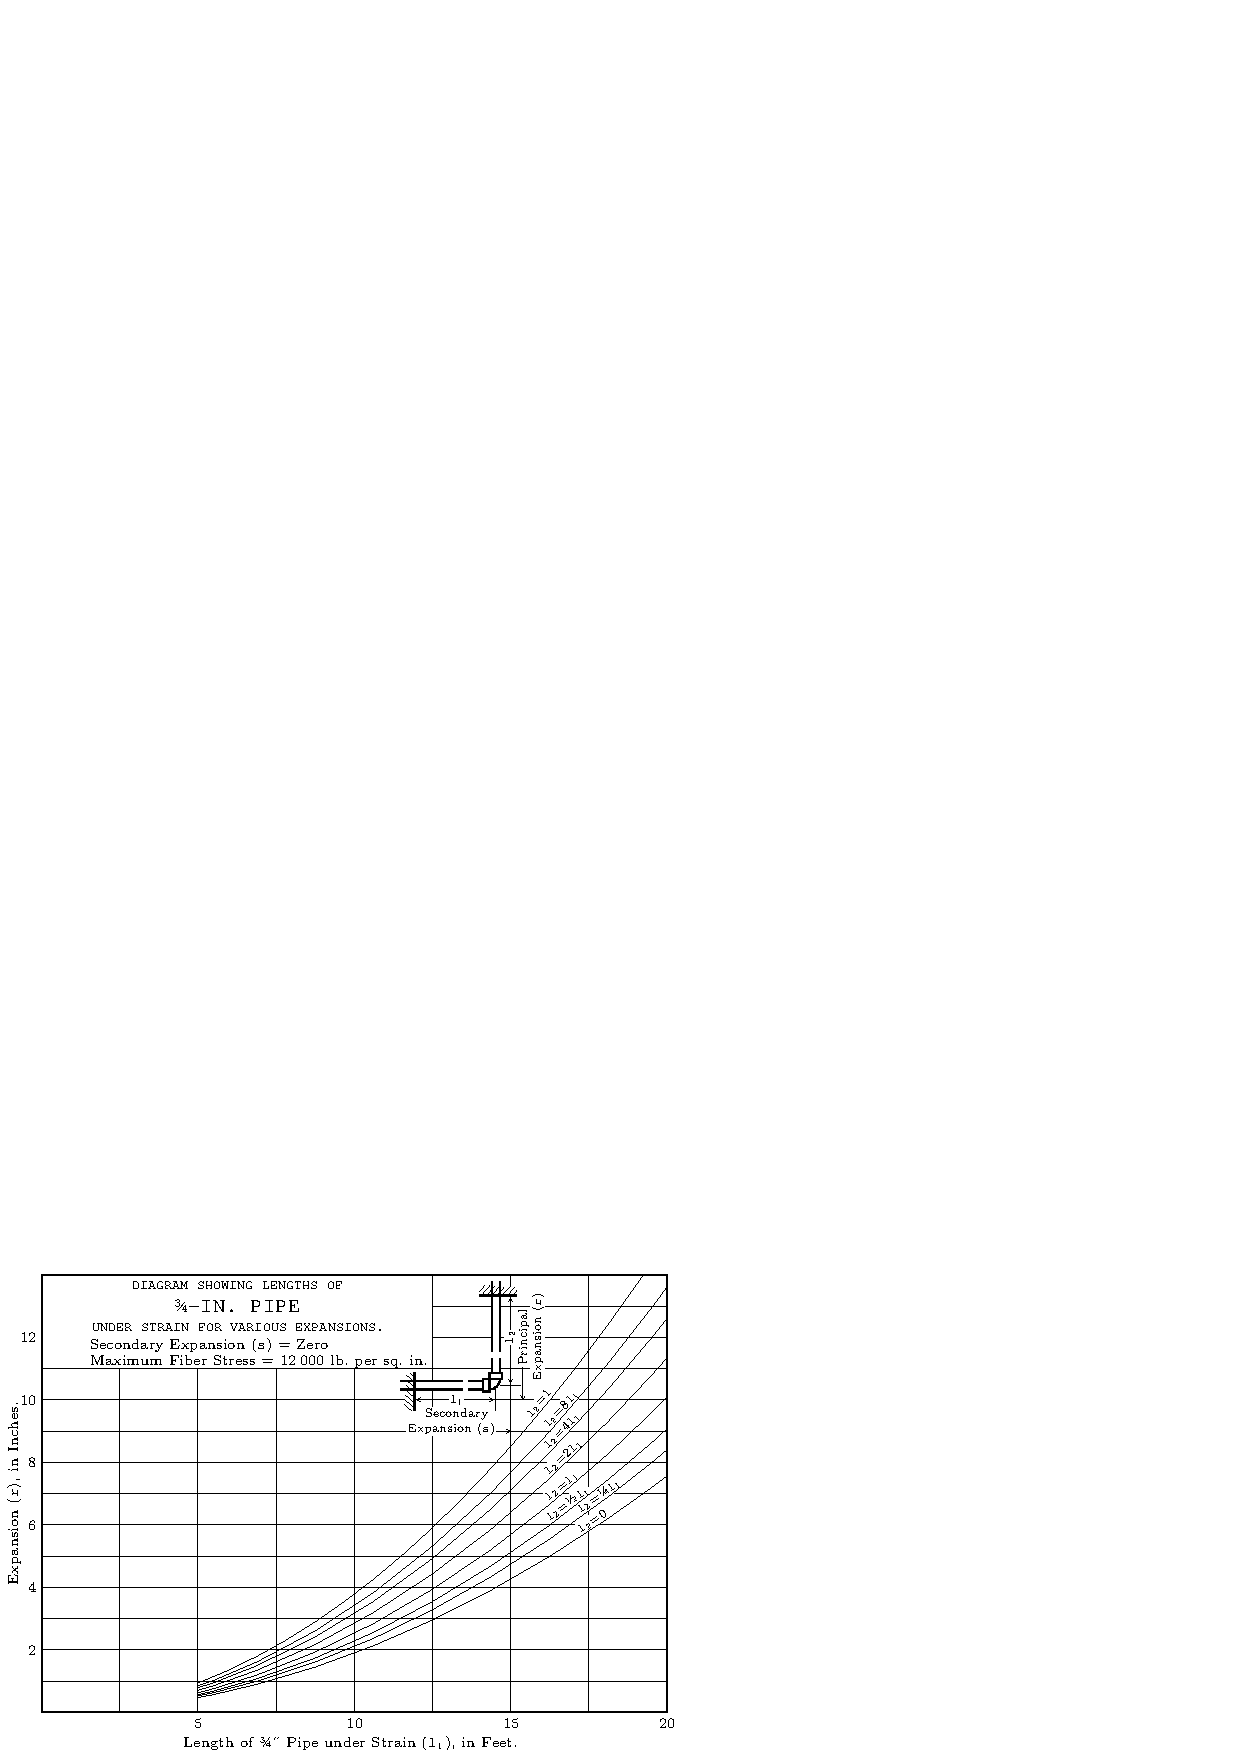
\includegraphics[width=.9\textwidth]{images/illus-013a}
%\textsc{Fig.~6.}]
\Legend{6}

\verybigskip

%[Illustration: Length of 1" Pipe under Strain ($l_1$), in Feet.
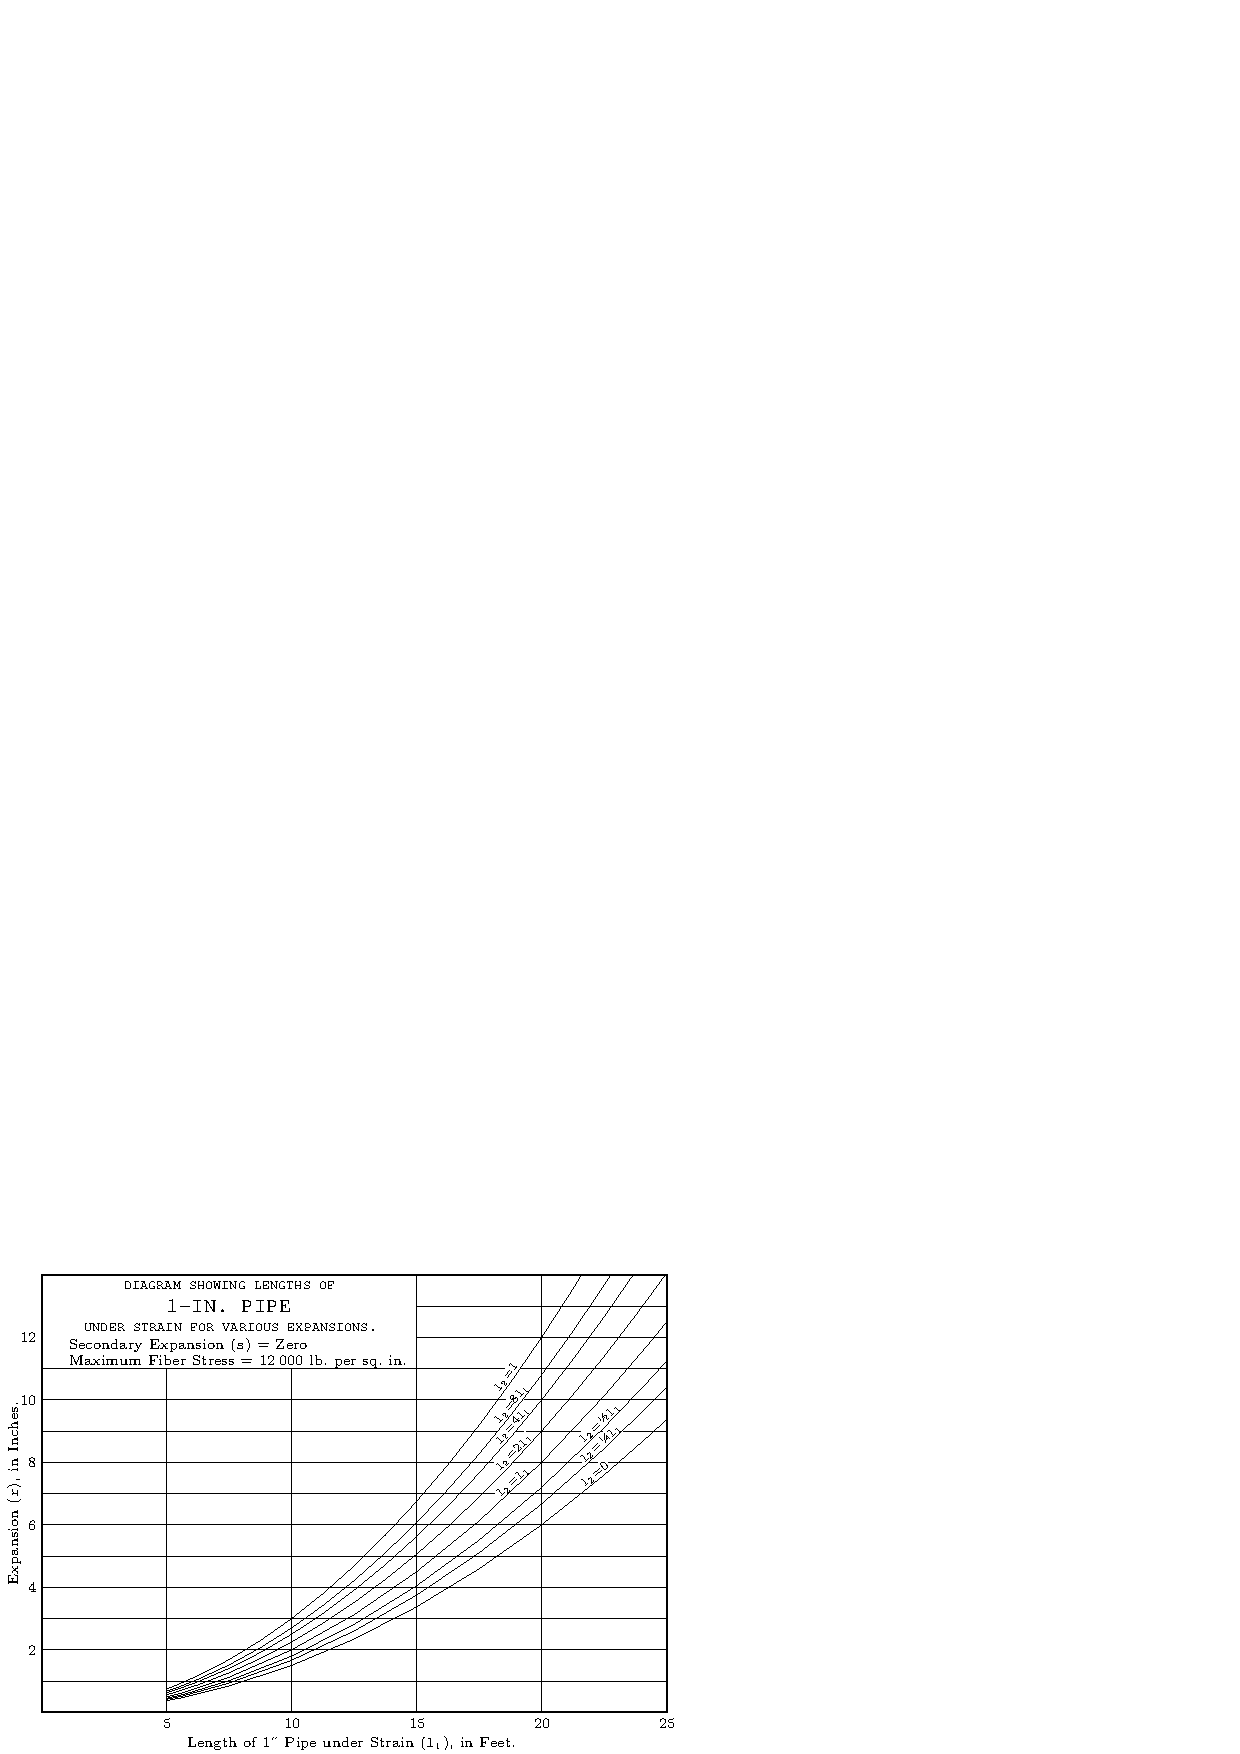
\includegraphics[width=.9\textwidth]{images/illus-013b}
%\textsc{Fig.~7.}]
\Legend{7}
\end{figure*}

\PGx--File: 014.png---\*********\*******\************\******\---------------

\begin{figure*}[p]
\centering
%[Illustration: Length of 1�" Pipe under Strain ($l_1$), in Feet.
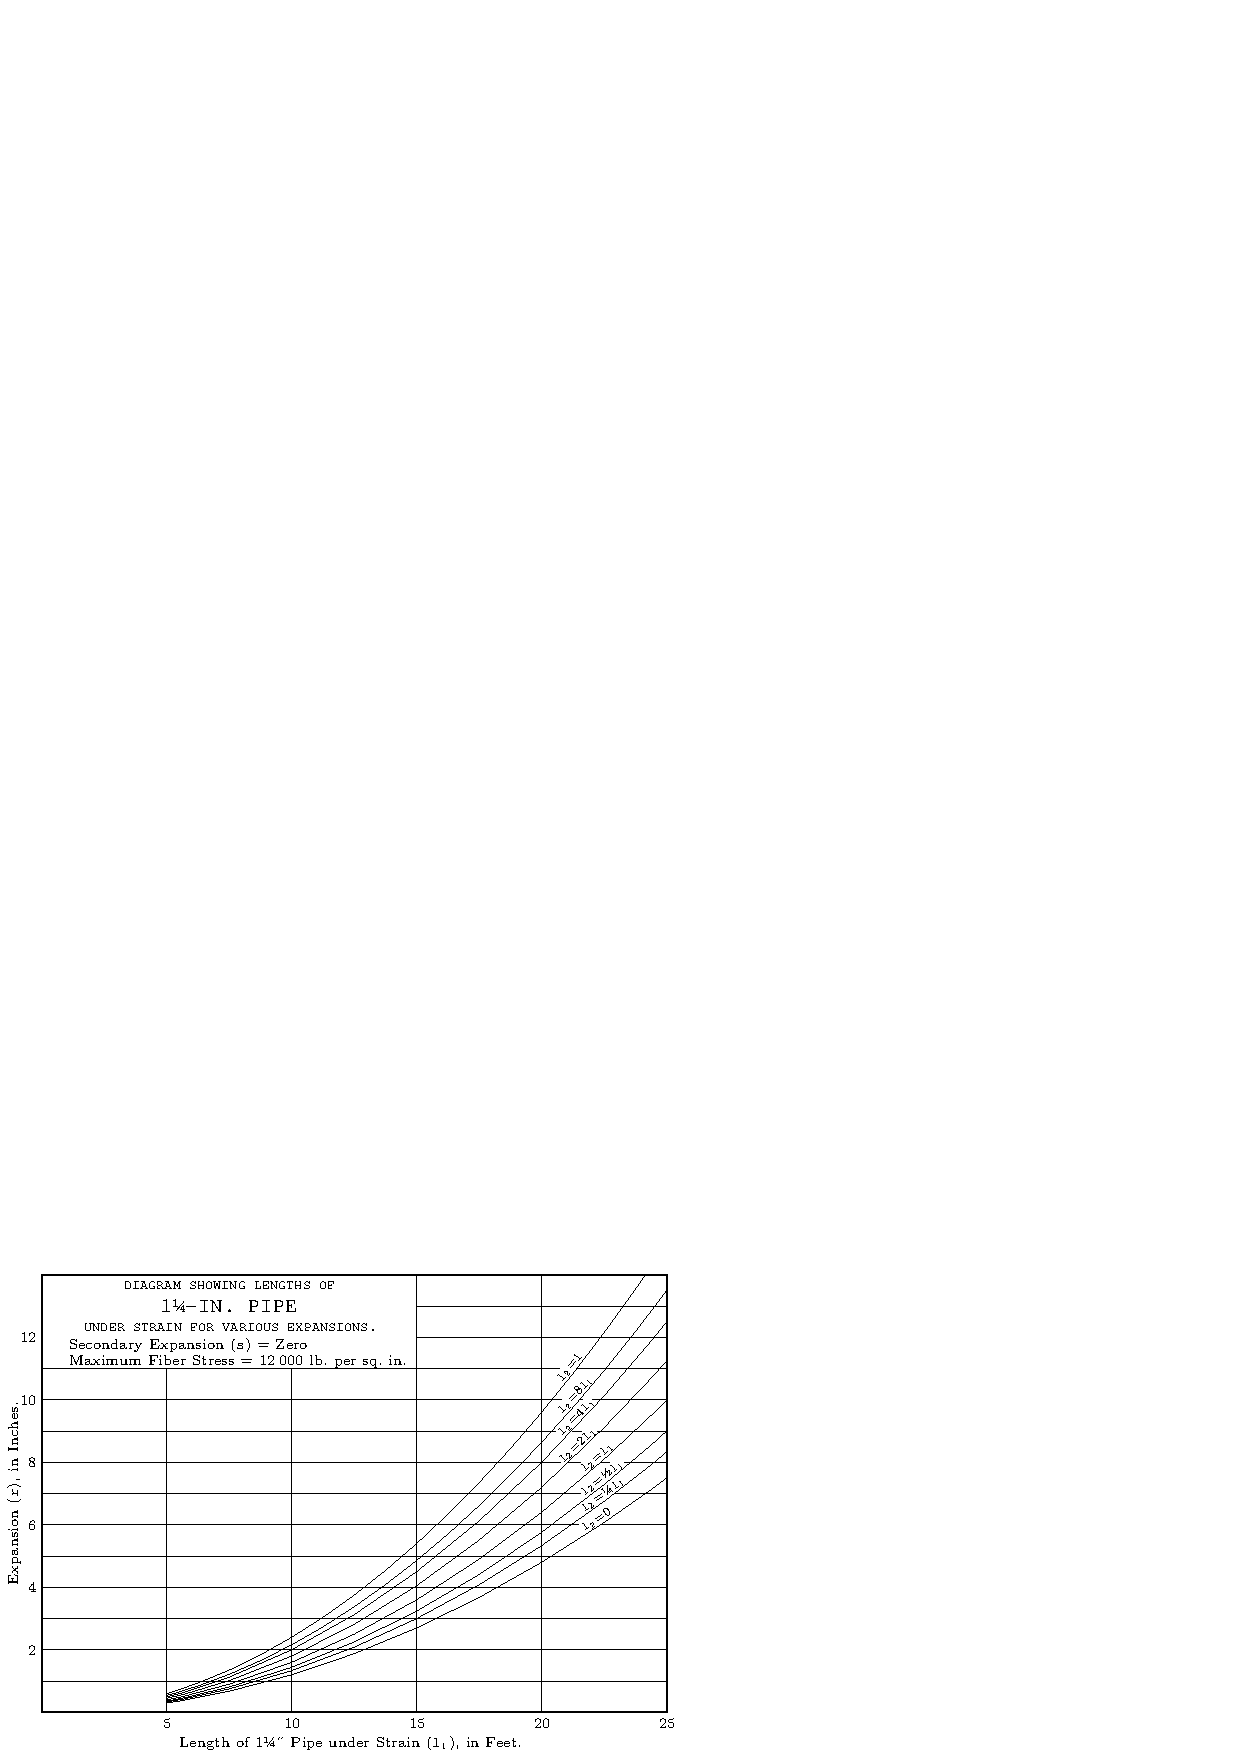
\includegraphics[width=.9\textwidth]{images/illus-014a}
%\textsc{Fig.~8.}]
\Legend{8}

\verybigskip

%[Illustration: Length of 1�" Pipe under Strain ($l_1$), in Feet.
%[Illustration: Length of ${1^1\!/\!{}_2}''$ Pipe under Strain ($l_1$), in Feet.
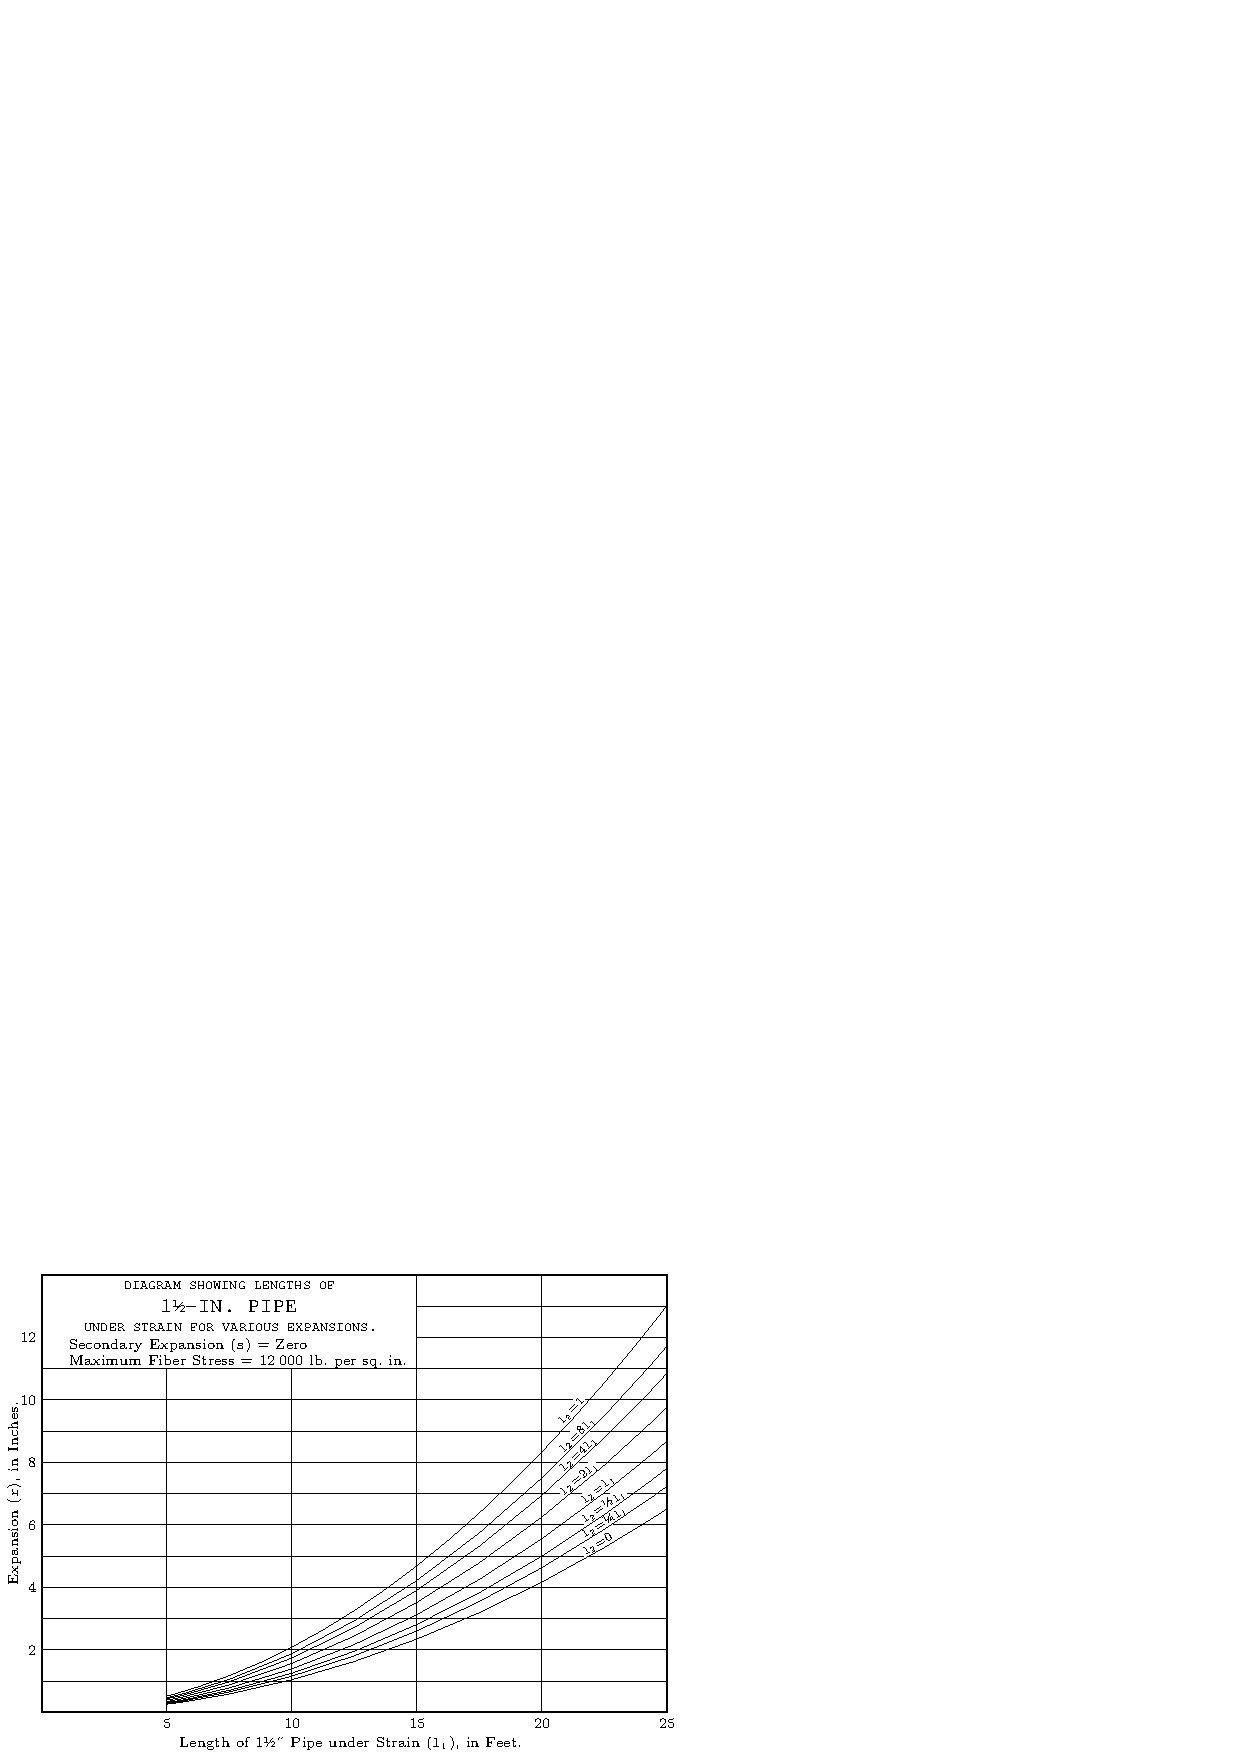
\includegraphics[width=.9\textwidth]{images/illus-014b}
%\textsc{Fig.~9.}]
\Legend{9}
\end{figure*}
\PGx--File: 015.png---\*********\*******\************\******\---------------
\begin{figure*}[p]
\centering
%[Illustration: Length of 2" Pipe under Strain ($l_1$), in Feet.
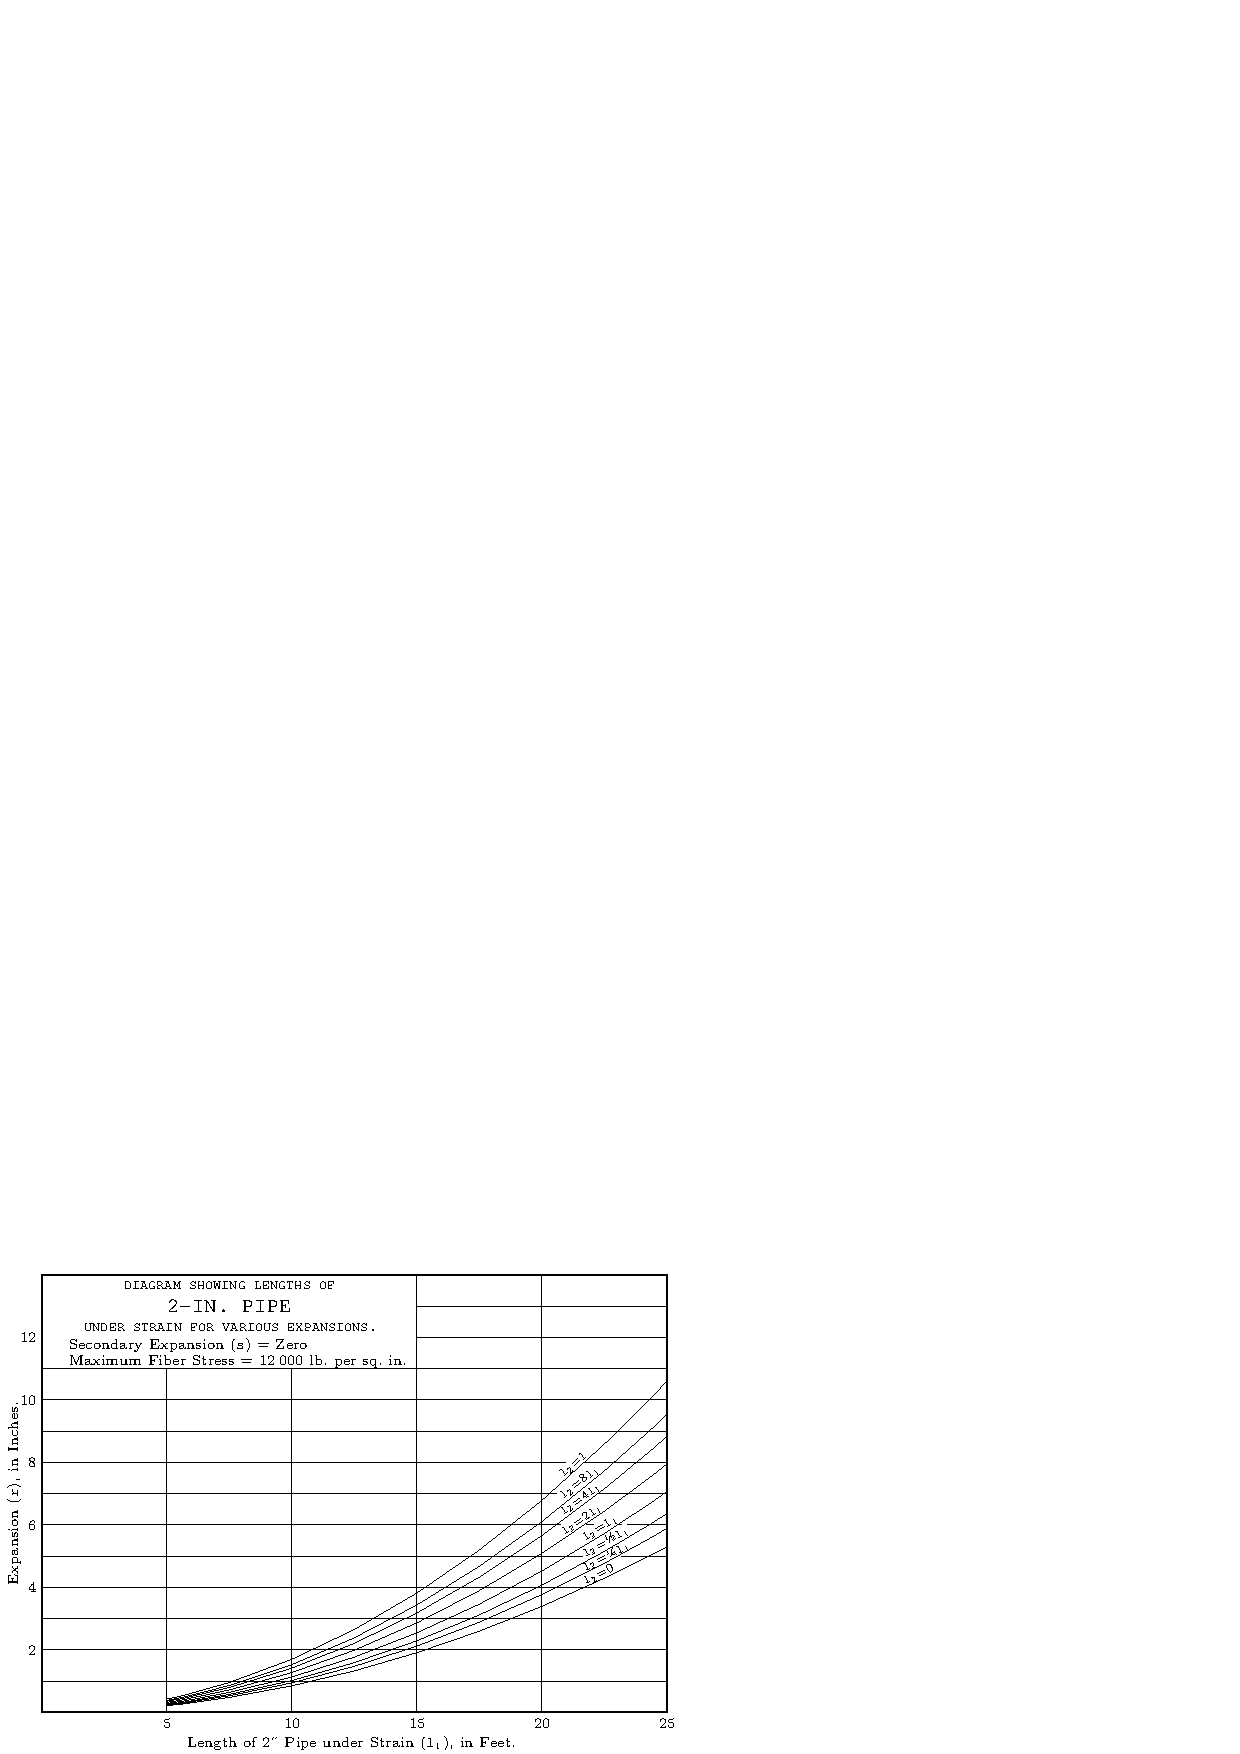
\includegraphics[width=.9\textwidth]{images/illus-015a}
%\textsc{Fig.~10.}]
\Legend{10}

\verybigskip

%[Illustration: Length of 2�" Pipe under Strain ($l_1$), in Feet.
%[Illustration: Length of ${2^1\!/\!{}_2}''$ Pipe under Strain ($l_1$), in Feet.
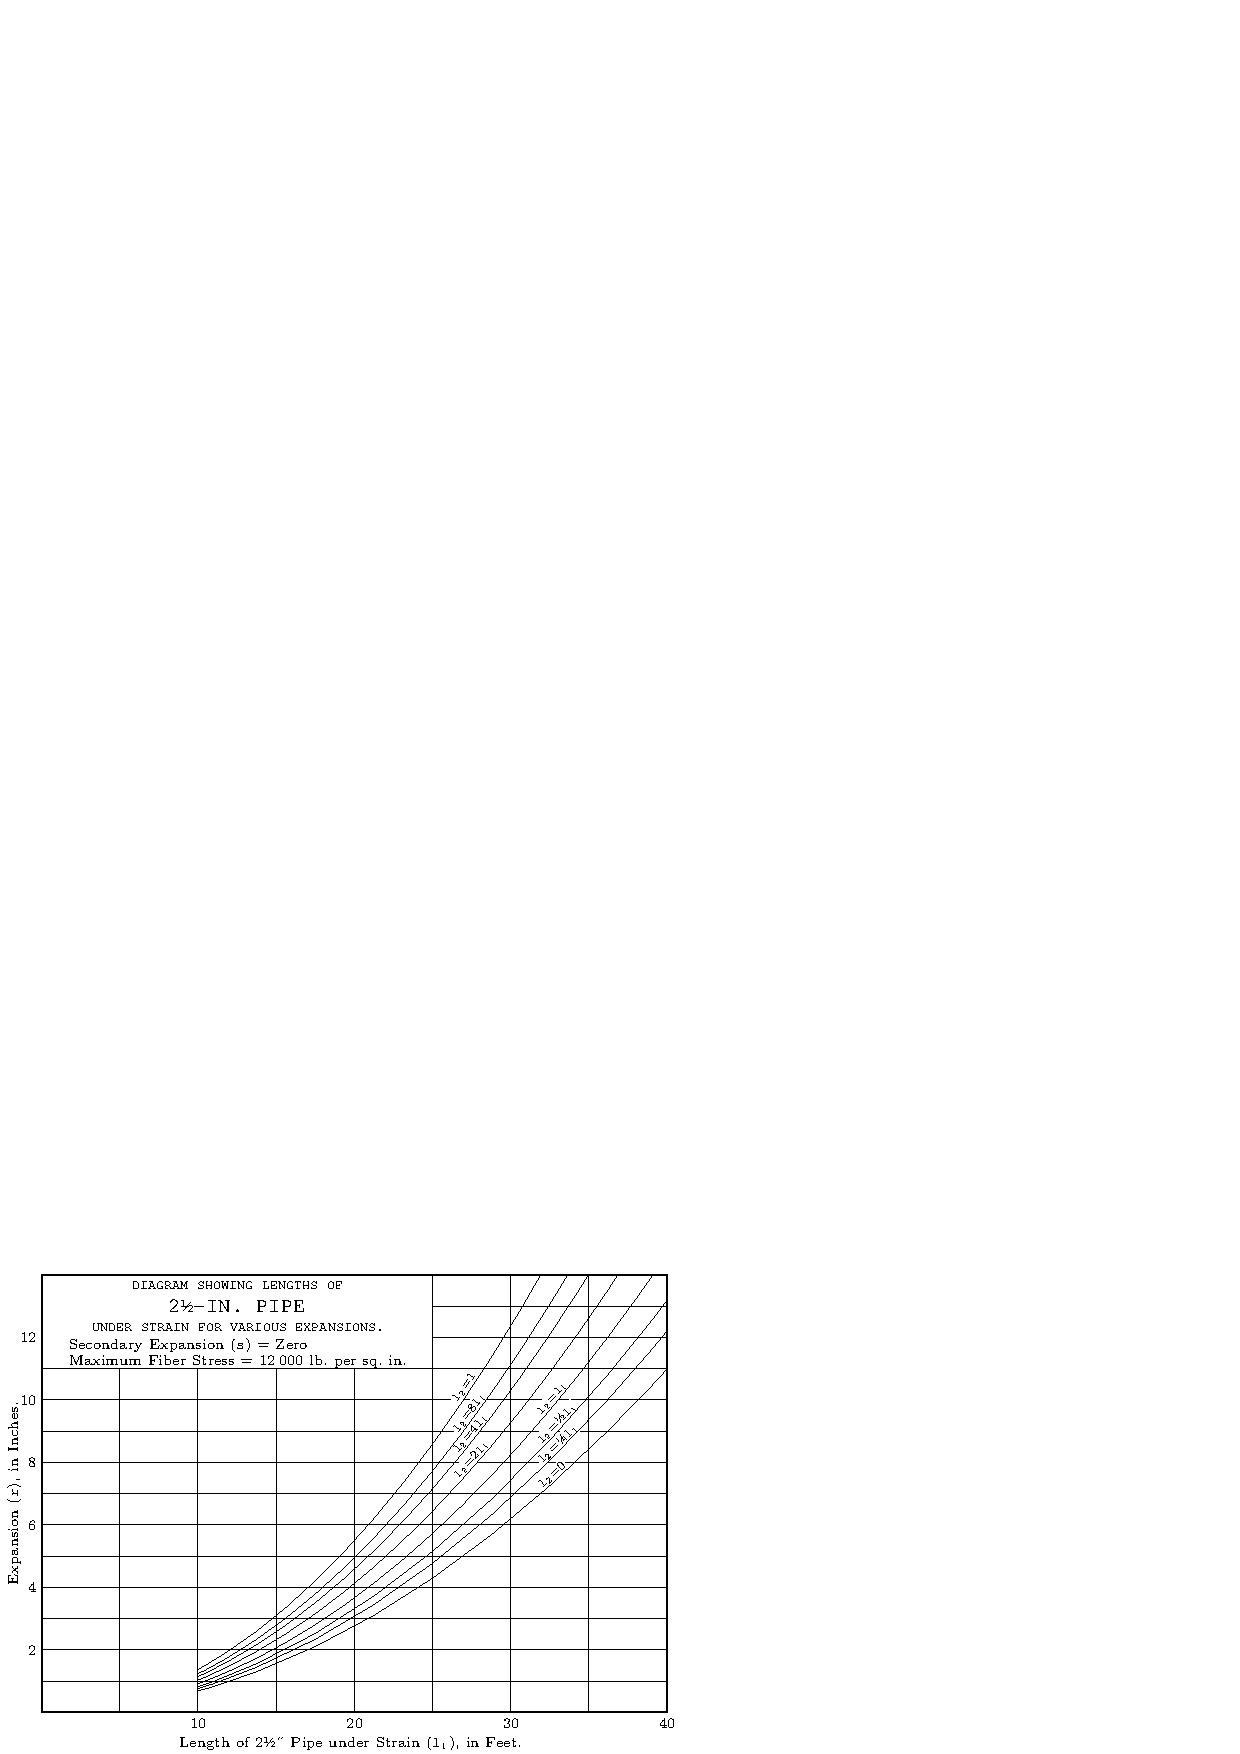
\includegraphics[width=.9\textwidth]{images/illus-015b}
%\textsc{Fig.~11.}]
\Legend{11}
\end{figure*}

\PGx--File: 016.png---\*********\*******\************\******\---------------

\begin{figure*}[p]
\centering
%[Illustration: Length of $3''$ Pipe under Strain ($l_1$), in Feet.
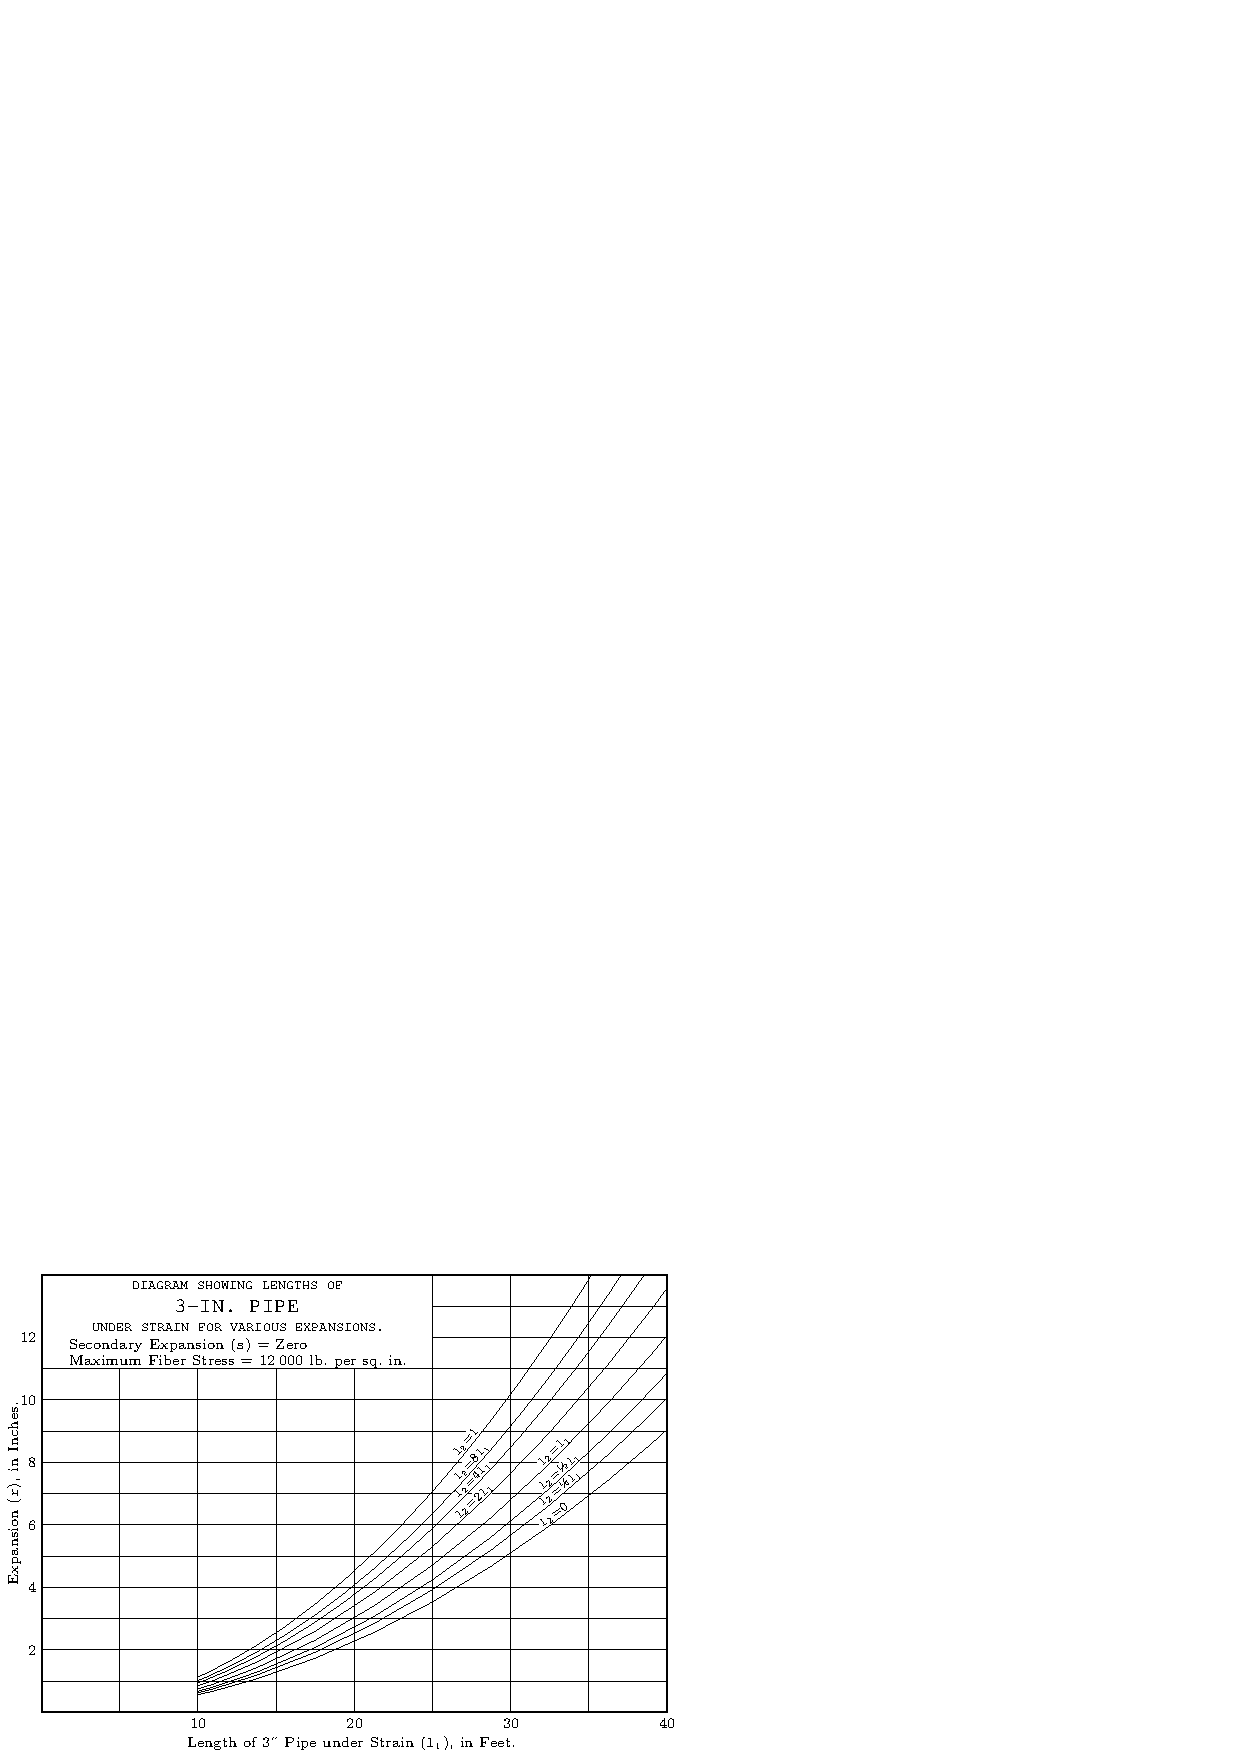
\includegraphics[width=.9\textwidth]{images/illus-016a}
%\textsc{Fig.~12.}]
\Legend{12}

\verybigskip

%[Illustration: Length of $4''$ Pipe under Strain ($l_1$), in Feet.
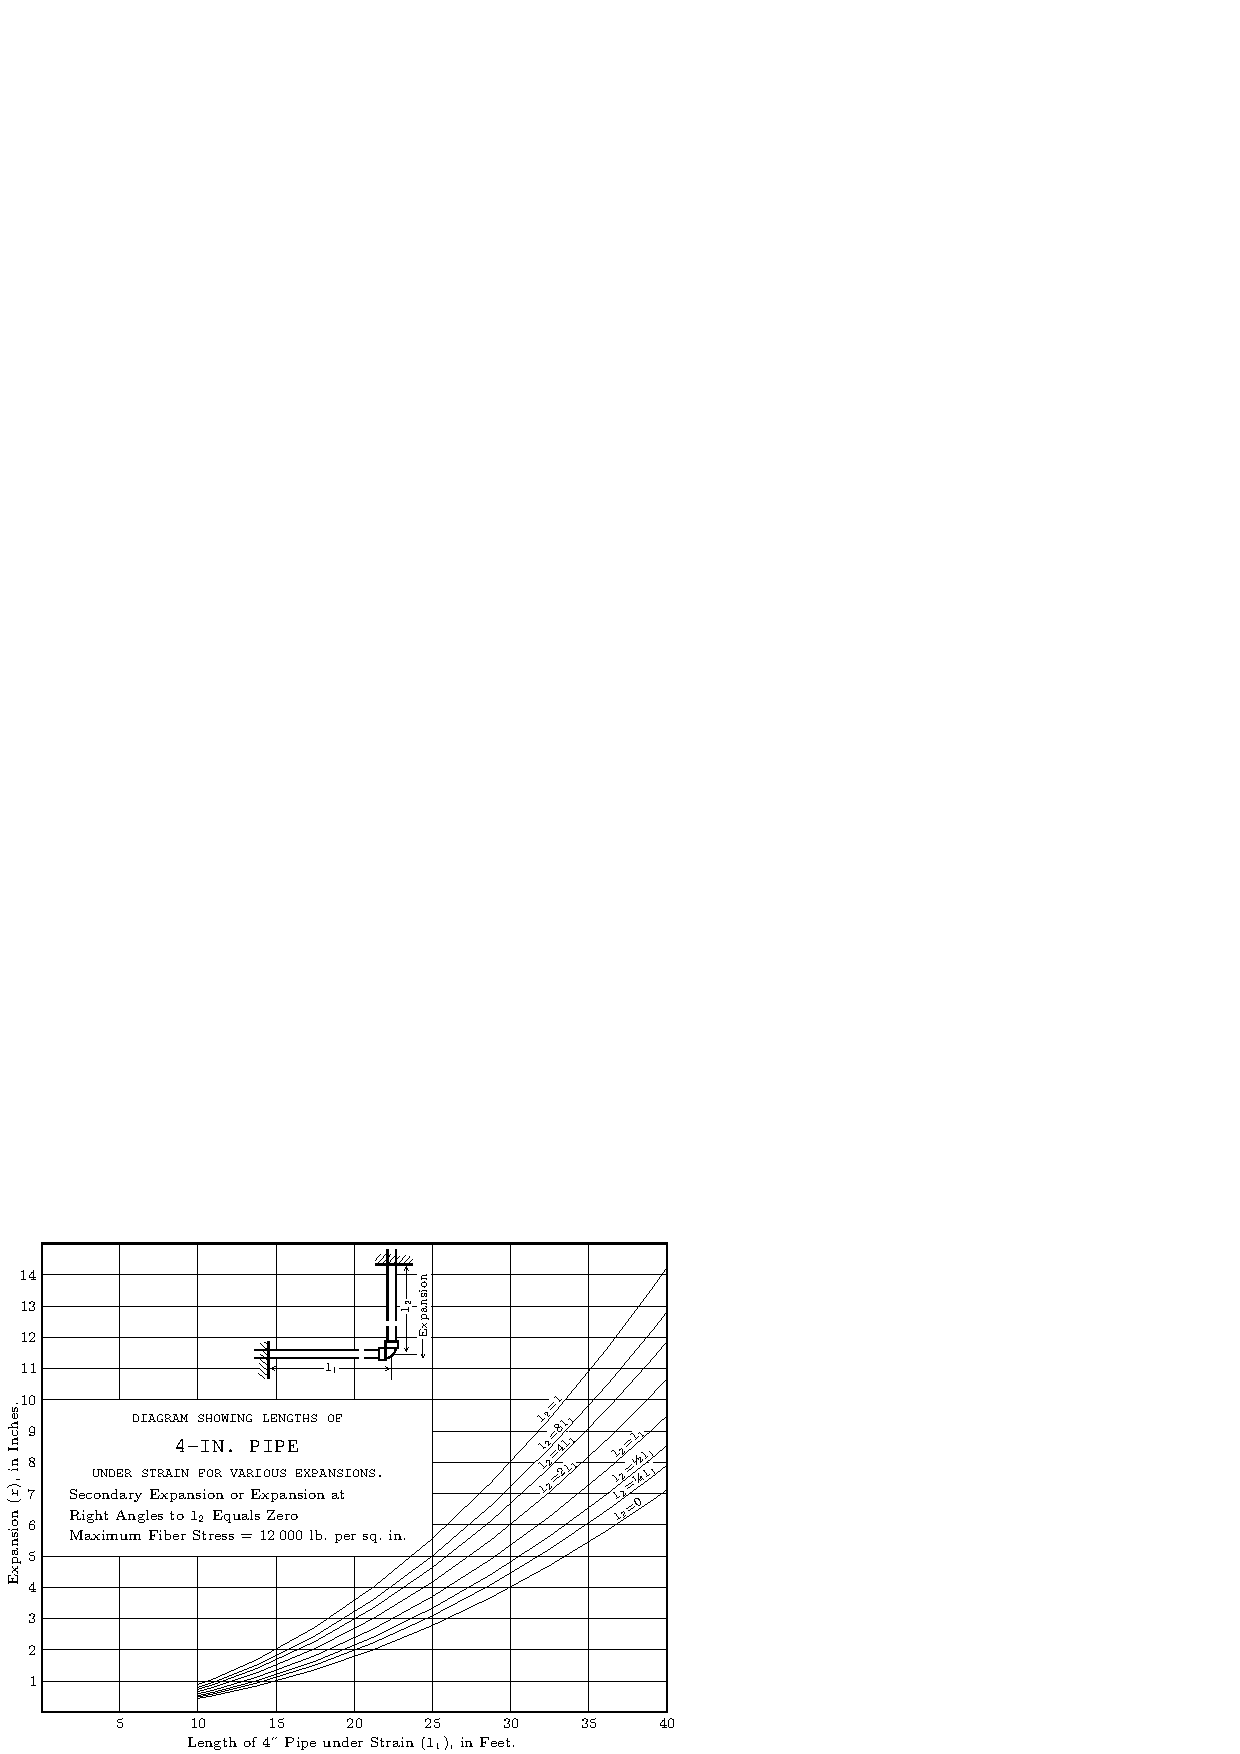
\includegraphics[width=.9\textwidth, viewport=0 0 330 235]{images/illus-016b}
%\textsc{Fig.~13.}]
\Legend{13}
\end{figure*}

\PGx--File: 017.png---\*********\*******\************\******\---------------

\begin{figure*}[p]
\centering
%[Illustration: Length of $5''$ Pipe under Strain ($l_1$), in Feet.
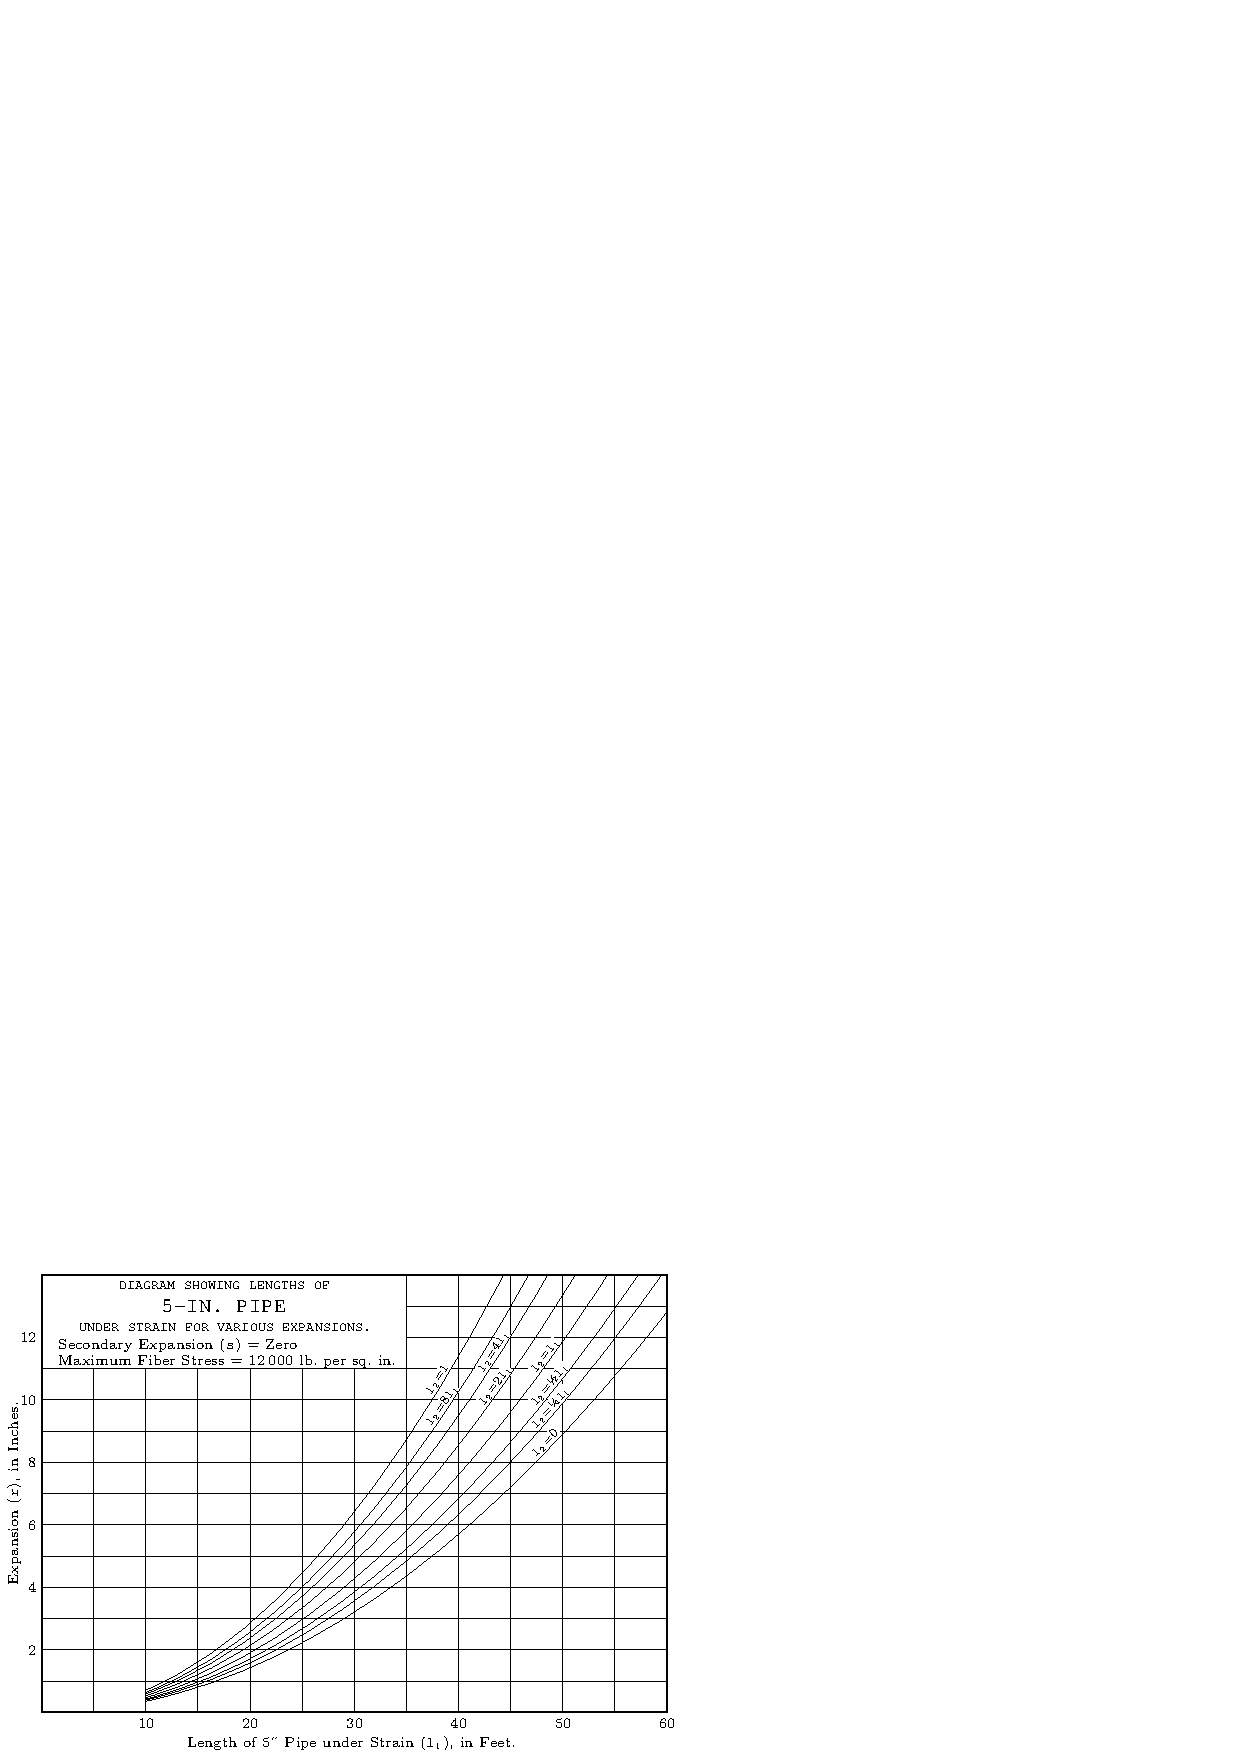
\includegraphics[width=.9\textwidth]{images/illus-017a}
%\textsc{Fig.~14.}]
\Legend{14}

\verybigskip

%[Illustration: Length of $6''$ Pipe under Strain ($l_1$), in Feet.
\includegraphics[width=.9\textwidth]{images/illus-017b}
%\textsc{Fig.~15.}]
\Legend{15}
\end{figure*}

\PGx--File: 018.png---\*********\*******\************\******\---------------

\begin{figure*}[p]
\centering
%[Illustration: Length of $8''$ Pipe under Strain (l_1), in Feet.
\includegraphics[width=.9\textwidth]{images/illus-018a}
%\textsc{Fig.~16.}]
\Legend{16}

\verybigskip

%[Illustration: Length of 10''$ Pipe under Strain ($l_1$), in Feet.
\includegraphics[width=.9\textwidth]{images/illus-018b}
%\textsc{Fig.~17.}]
\Legend{17}
\end{figure*}

\PGx--File: 019.png---\*********\*******\************\******\---------------

\begin{figure*}[p]
\centering
%[Illustration: Length of $12''$ Pipe under Strain ($l_1$), in Feet.
\includegraphics[width=.9\textwidth]{images/illus-019a}
%\textsc{Fig.~18.}]
\Legend{18}

\verybigskip

%[Illustration: Length of $14''$ Pipe under Strain ($l_1$), in Feet.
\includegraphics[width=.9\textwidth]{images/illus-019b}
%\textsc{Fig.~19.}]
\Legend{19}
\end{figure*}

\PGx--File: 020.png---\*********\*******\************\******\---------------

\begin{figure*}[p]
\centering
%[Illustration: Length of $16''$ Pipe under Strain ($l_1$), in Feet.
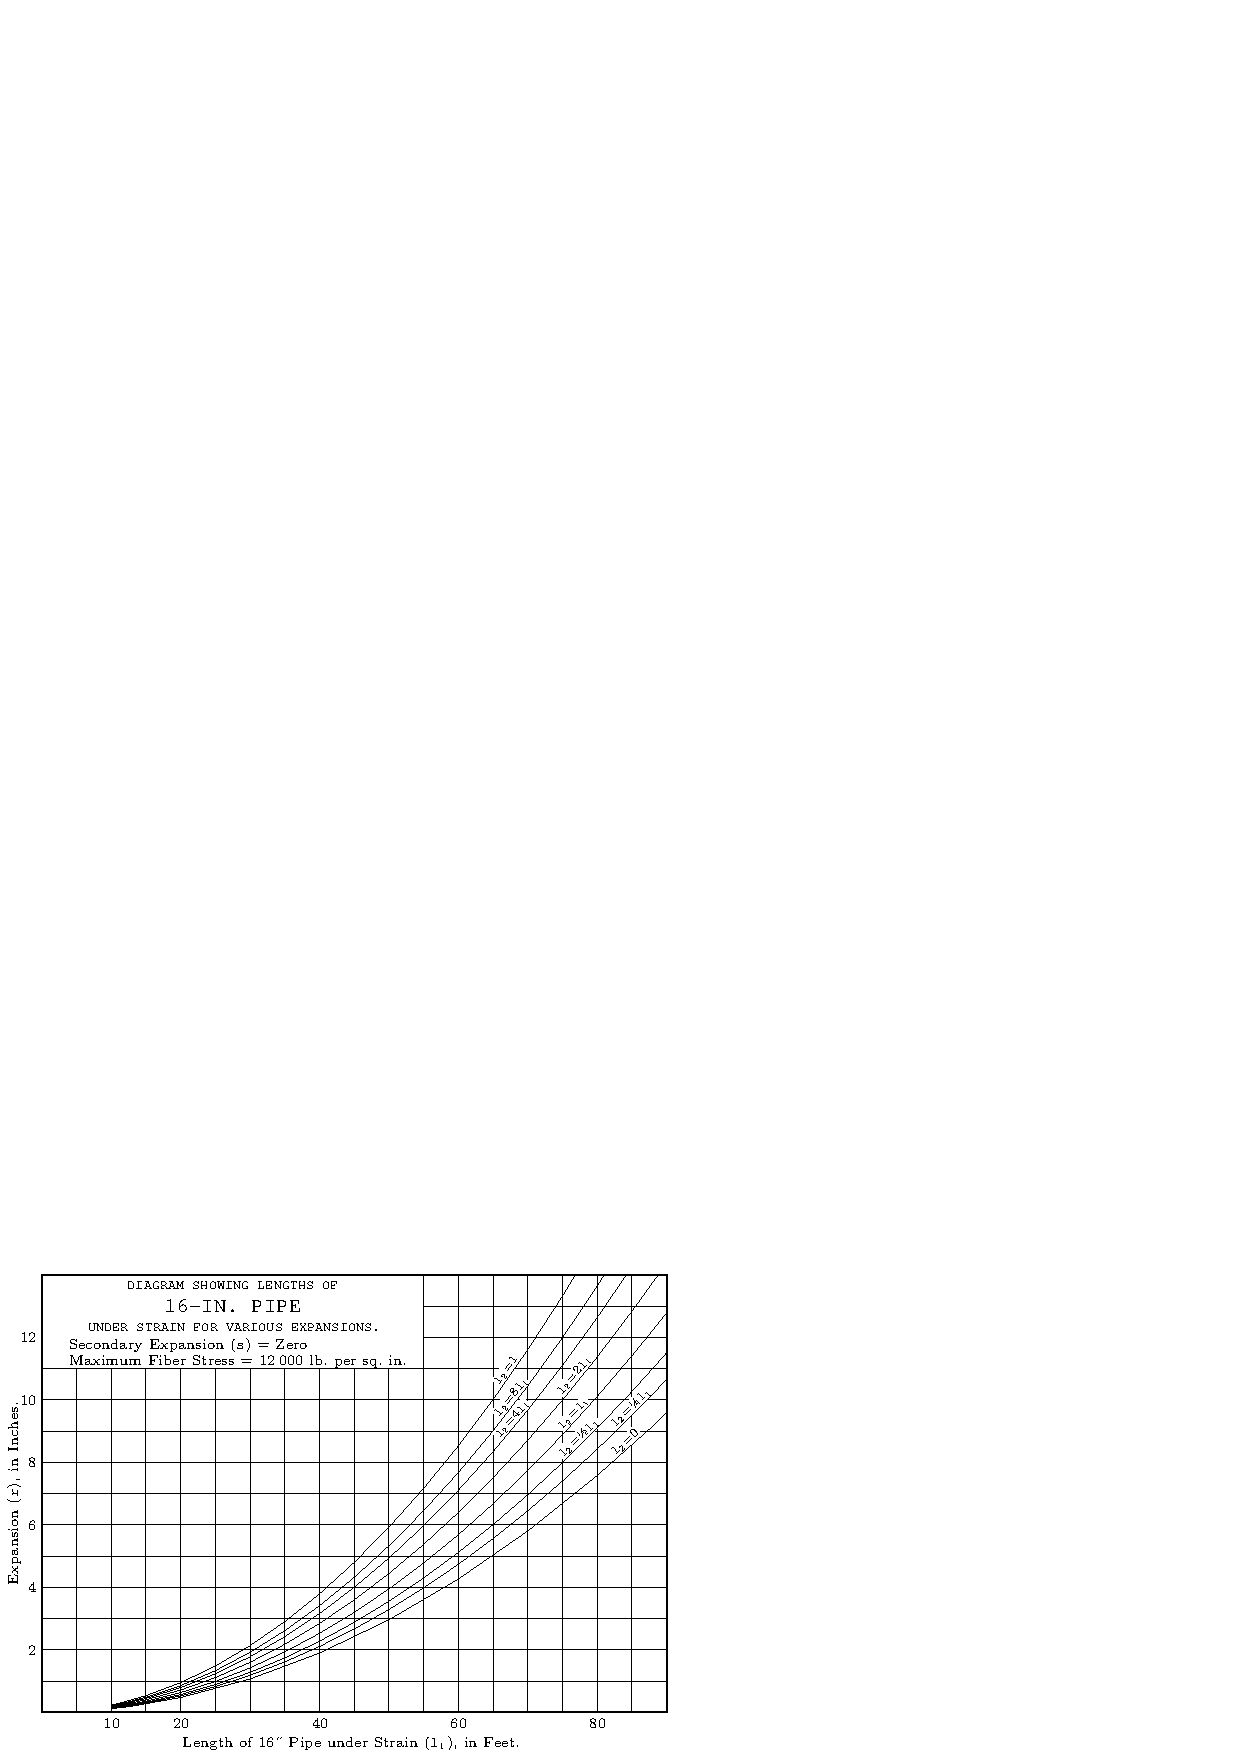
\includegraphics[width=.9\textwidth]{images/illus-020a}
%\textsc{Fig.~20.}]
\Legend{20}

\verybigskip

%[Illustration: Length of $18''$ Pipe under Strain ($l_1$), in Feet.
\includegraphics[width=.9\textwidth]{images/illus-020b}
%\textsc{Fig.~21.}]
\Legend{21}
\end{figure*}

\PGx--File: 021.png---\*********\*******\************\******\---------------

\begin{figure*}[p]
\centering
%[Illustration: Length of $20''$ Pipe under Strain ($l_1$), in Feet.
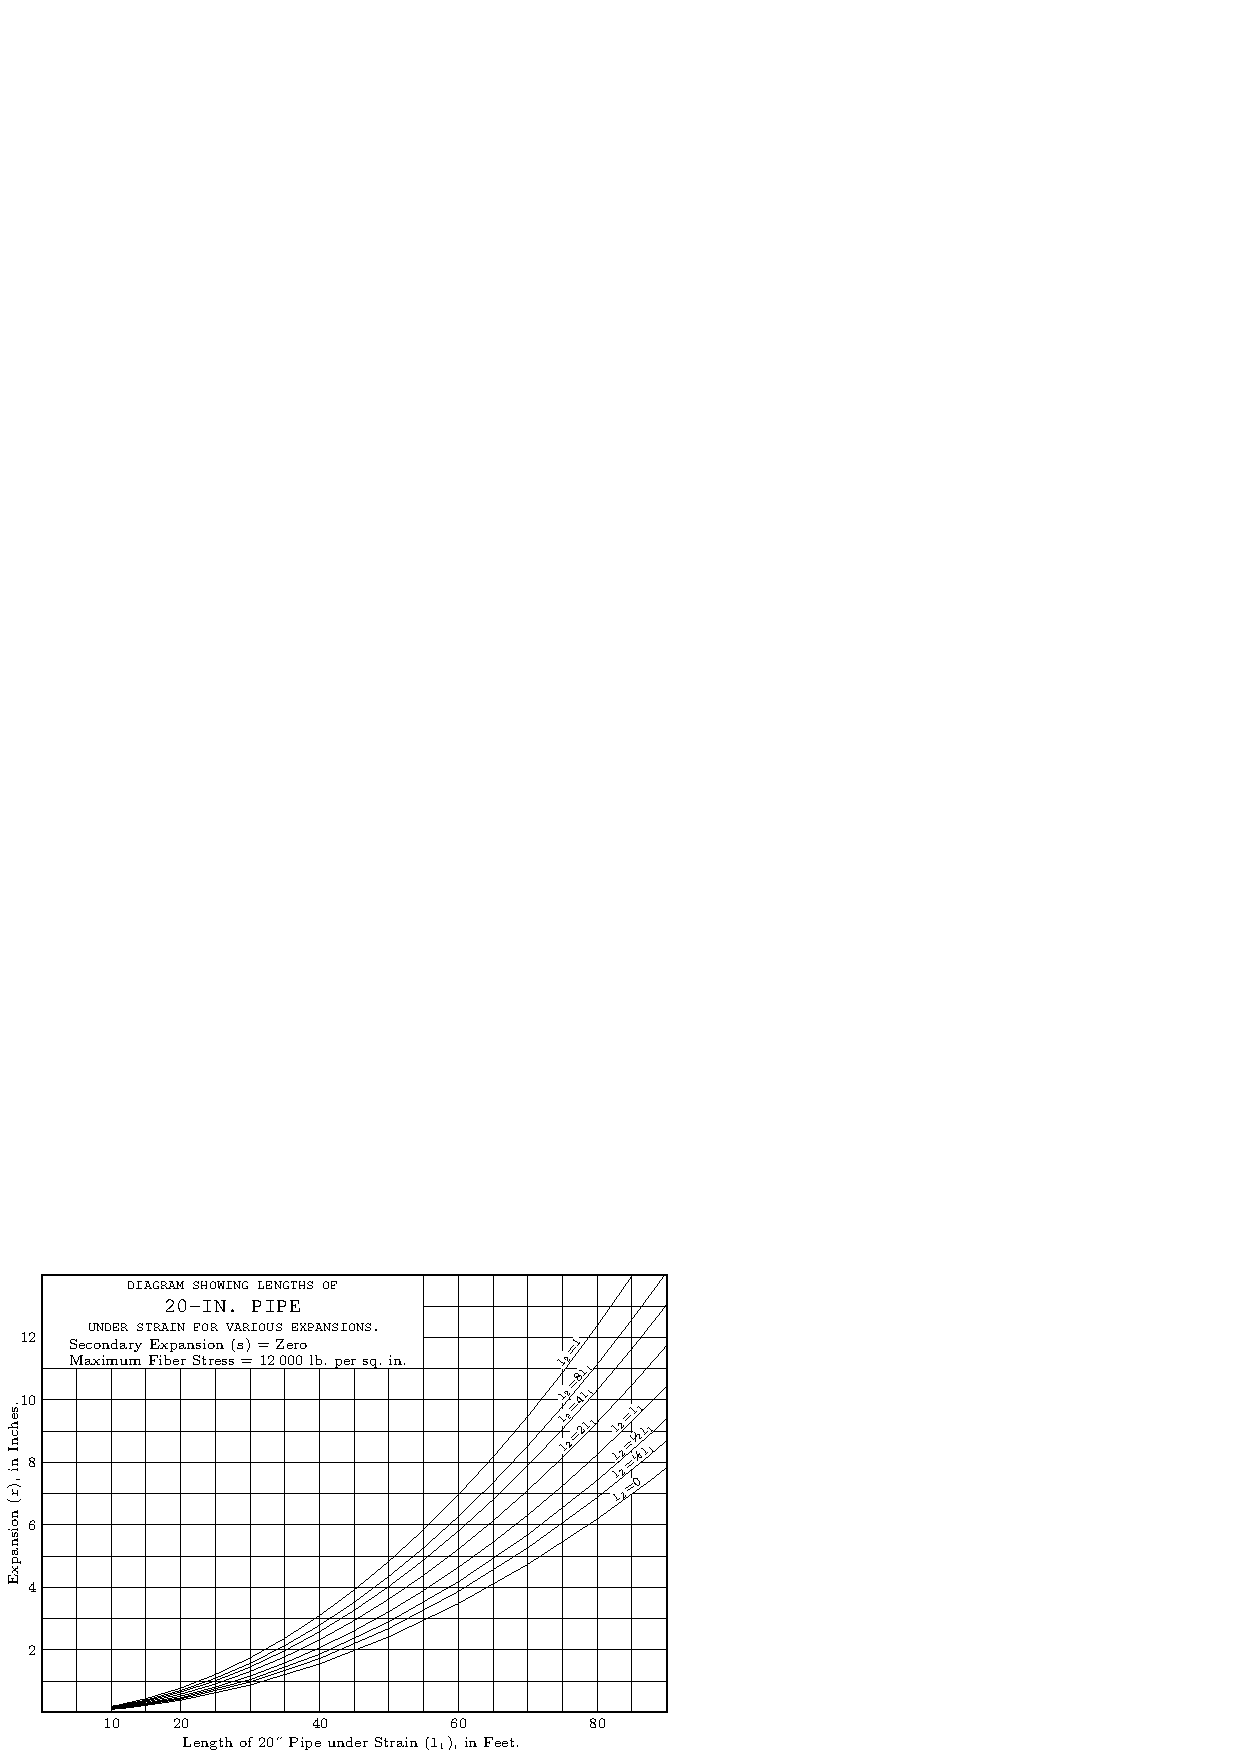
\includegraphics[width=.9\textwidth]{images/illus-021a}
%\textsc{Fig.~22.}]
\Legend{22}

\verybigskip

%[Illustration: Values of $\frac{s}{r}$, Secondary Expansion $\div$ Principal Expansion.
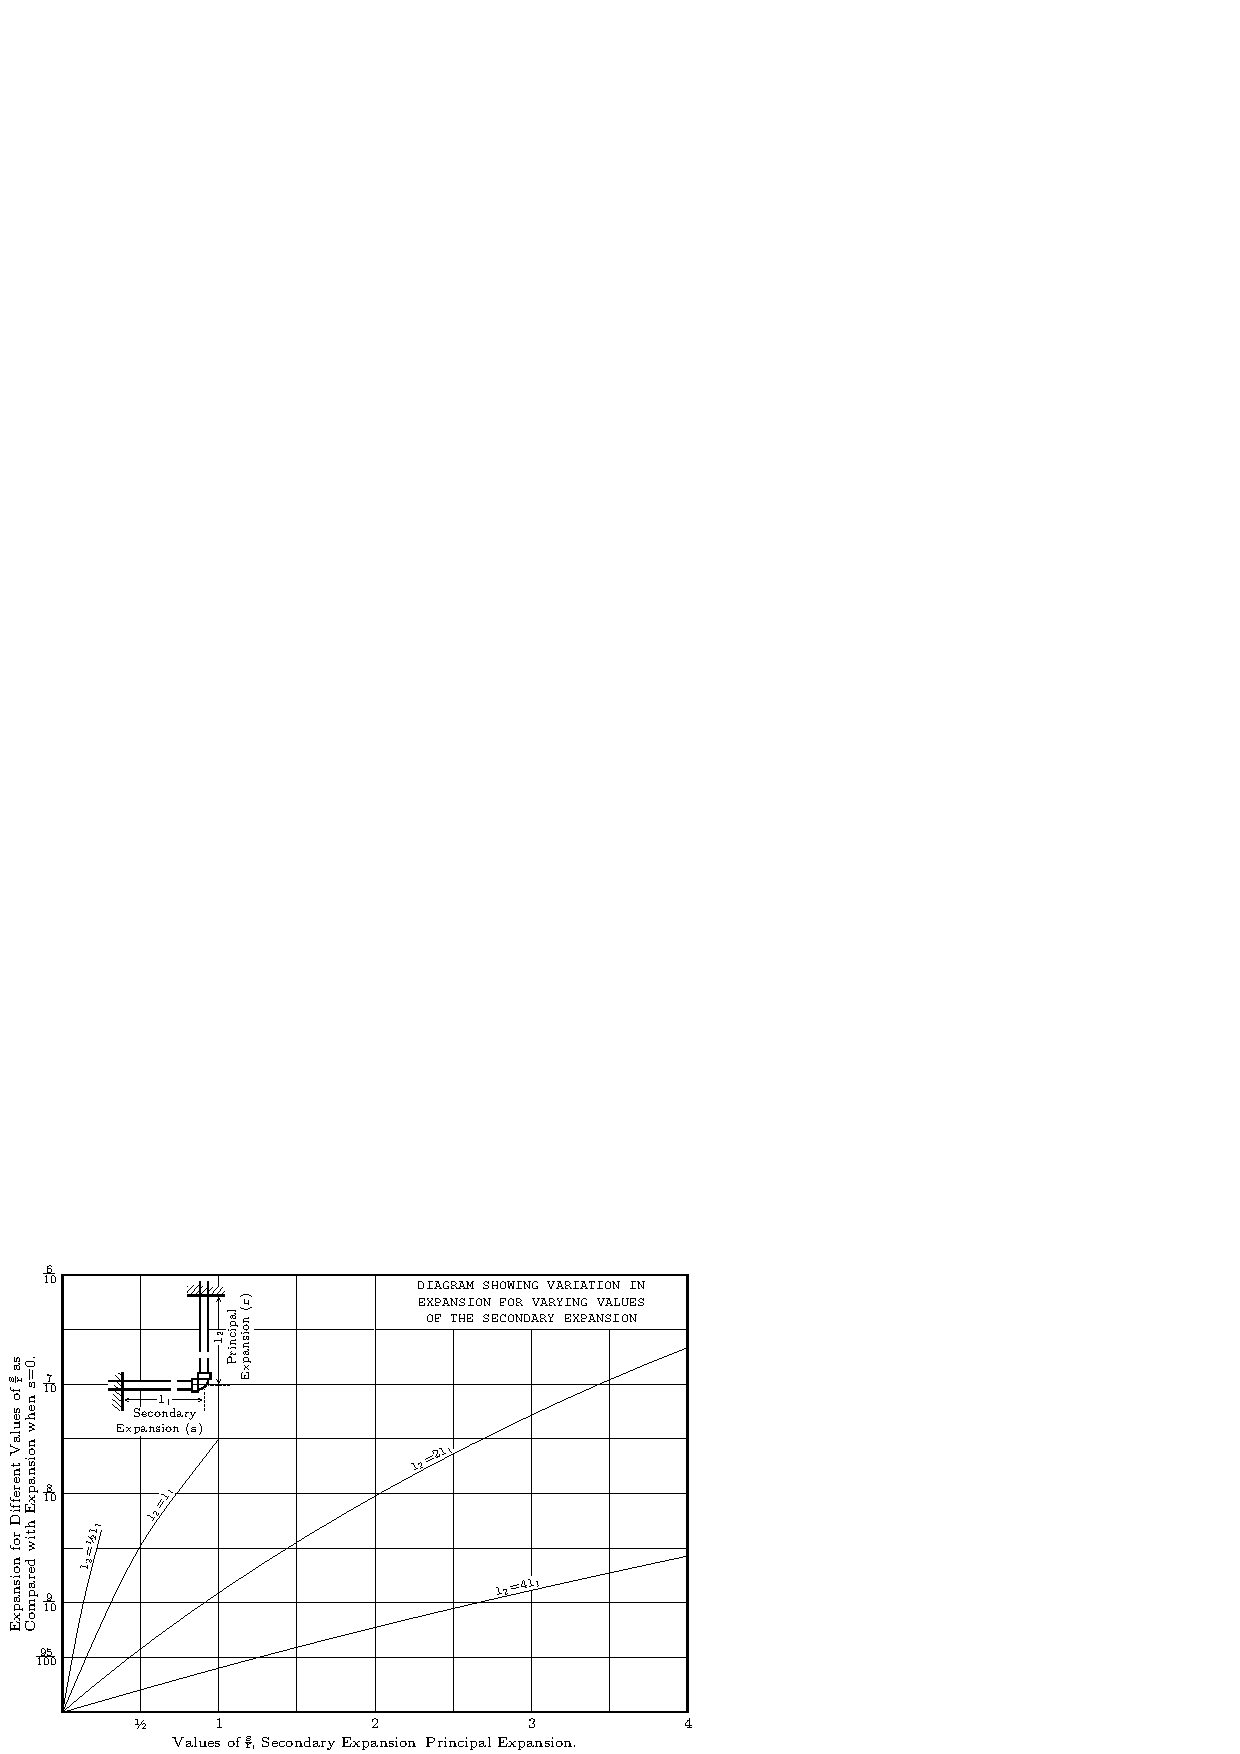
\includegraphics[width=.9\textwidth, viewport=10 0 340 235]{images/illus-021b}
%\textsc{Fig. 23.}]
\Legend{23}
\end{figure*}

\PGx--File: 022.png---\*********\*******\************\******\---------------

\begin{figure*}[p]
\centering
%[Illustration: Values of $\frac{s}{r}$, Secondary Expansion $\div$ Principal Expansion.
\includegraphics[width=.9\textwidth, viewport=10 0 340 235]{images/illus-022a}
%\textsc{Fig.~24.}]
\Legend{24}

\verybigskip

%[Illustration: Values of $\frac{s}{r}$, Secondary Expansion $\div$ Principal Expansion.
\includegraphics[width=.9\textwidth]{images/illus-022b}
%\textsc{Fig.~25.}]
\Legend{25}
\end{figure*}

% first 5 lines moved from 012.png to join up paragraph
Consider first the expansion in a 4-in.\ pipe, where the principal
expansion is 6~in., and where the secondary expansion (or that at right
angles to the principal expansion), is negligible. This length can be
determined directly from \figref{13}. If $l_2$ is zero, the length of $l_1$ will
be 37~ft. If $l_2$ equals 10~ft., it will be more than $\dfrac{l_1}{4}$, because $l_1$ must
\PG--File: 023.png---\*********\*******\************\******\---------------
equal something less than 37~ft., if $l_2$ has any value at all. With $l_2$
equal to 10~ft., $l_2$ is more than $\dfrac{l_1}{4}$ and undoubtedly less than $\dfrac{l_1}{2}$. If $l_2$
equals $\dfrac{l_1}{2}$, it will be seen from \figref{13}, that $l_1$ will be a little less than
34~ft., and if $l_2$ equals $\dfrac{l_1}{4}$, $l_1$ equals 35~ft. It will be seen, therefore,
that $l_2$ is about two-sevenths of $l_1$ or nearly $\dfrac{l_1}{4}$, and that $l_1$ should be
taken as $34\frac12$ or 35~ft.

If the length, $l_2$, becomes equal to $8l_1$, it will be seen from \figref{13}
that $l_1$ should equal $27\frac12$~ft. When $l_2$ becomes very long, the fact as to
whether it can move freely must, of course, be taken into consideration.
If it must slip over fixed supports, the friction of slippage will, of
course, have the same effect as the shortening of the length, $l_2$. On
the other hand, it often happens that pipes passing through walls, or
in similar conditions, will be held so as to permit of some slight side
movement, although it may not be allowed for in the calculations.
This, of course, would have the same effect as an increase in the length
of pipe under strain.

Let us now consider the expansion in a 4-in.\ pipe where the
principal expansion is 6~in., the secondary expansion is 3~in., and the
lengths of $l_1$ and $l_2$ are to be equal. From \figref{24}\footnoteT
  {The curve for $l_2=4l_1$ in Fig.~24 has been corrected.
   The original figure showed the curve passing through $(2,1.05)$}, it will be seen,
when the principal expansion divided by the lesser or secondary expansion
$( \text{or }\dfrac{s}{r})=\dfrac12$, % shrinking parentheses to normal text size
and when $l_1=l_2$, that (compared with the
case where the secondary expansion equals zero) the lengths should be
increased in the ratio of 1 to 1.085, or, from \figref{23}, it will be seen
that the expansion should be decreased in the ratio of 1 to 0.85.

From \figref{13} it will be seen that $l_1$ should be nearly 32~ft.\ for a
4-in.\ pipe with a 6-in.\ expansion (the secondary expansion being zero
and $l_1=l_2$). If, in addition to the principal expansion of 6~in., there
is a secondary expansion of 3~in., the lengths should be increased, as
before stated, in the ratio of 1 to 1.085, or 32~ft.\ should be changed
to nearly 35~ft. If, however, it is desired not to increase these lengths,
the lessened amount of expansion or the increased maximum fiber
stress can be determined. From \figref{23} it has been determined
that the expansion should be decreased in the ratio of 1 to 0.85, or
\PG--File: 024.png---\*********\********\************\******\--------------
6 and 3~in.\ should become 5.1 and 2.55~in., respectively. If, however,
it is desired to maintain the 6- and 3-in.\ expansion, it will be seen
from the equations that the fiber stress varies directly as the expansion,
and hence the maximum fiber stress will become\footnoteT{Original lacks `lb.'}
\[
  12\,000\times \frac{1}{0.85}=14\;118 \text{ lb.\ per sq.\ in.}
\]

There is one factor which has already been mentioned, to which,
however, further attention should be given, that is the question as to
how much allowance should be made for the weakening of a pipe at
a fitting due either to the strength of the fitting or the threads
on the pipe. In order to determine what this allowance should
be, we must make $\dfrac{fI}{\frac12 D}$, % shrinking fraction in denominator to text size as in (22)
in \hyperlink{eq:22}{Equation~22}, equal to the moment where
$X=kL$, instead of to $M_1$, where $X=0$. Following through similar
succeeding equations, we will secure the equation:
\begin{flalign*}
&&&\multispan{2}{\hfil$-r=\dfrac{f}{3ED}L^2k(k-1)-hk$\hfil}&&
\Tag{34}\\
&\rlap{or}&&
\multispan{2}{\hfil$
r+s\dfrac{k}{1-k}=\dfrac{f{l_1}^2}{3EDk}$.\hfil}&&
\Tag{35}
\end{flalign*}
The comparative values of the pipe strain at the joint and the fixed
point of the pipe, have been determined from \hyperlink{eq:35}{Equation~35}, and are
shown graphically in \figref{25}.

In using this diagram in the following discussion, the loss in strength
at the elbow is calculated as one-third. Therefore, an allowance
should be made for the weakening at the fitting when the maximum
strain is less than $\dfrac{1}{1-\frac{1}{3}}$, % shrinking fraction in denominator to text size
or $1\frac12$ times the strain at the elbow. An
examination of the curves on \figref{25} will show that this is practically
always the case when $l_2=l_1$, or anything less than $l_1$. It is also the
case when $l_2=2l_1$, and the secondary is equal to or larger than the
principal expansion. It will be remembered that the principal expansion
is usually larger than $\Bigl(\dfrac{l_1}{l_2}\Bigr)^{\!2}$ times the secondary expansion, where $l_1$
is the length of pipe under strain at right angles to the direction of
the principal expansion, and $l_2$ is the length of pipe under strain at
right angles to the secondary expansion, but the principal expansion
is not necessarily larger in quantity than the secondary expansion.
\PG--File: 025.png---\*********\********\************\******\--------------

The allowance will depend on the ratio of the maximum strain to
the strain at the elbow, which values are shown by the curves in
\figref{25}. When $l_2=0$, the strain at the elbow equals the strain at
the point where the pipe is held in line, and the strain at all intermediate
points is also the same. The allowance for the weakening
at the elbow, or for any joint between the elbow and the point where
the pipe is held in line, therefore, should be in the ratio of 1 to $1\frac12$ or
the strain allowable should be two-thirds of what otherwise might be
calculated when $l_2=0$.

If $l_2$ has some other value, for example, if $l_2=2l_1$, and if $\dfrac{s}{r}=2$,
it will be seen, from \figref{25}, that the maximum strain is $1\frac14$ times
the strain at the elbow. If we calculate the elbow to be only two-thirds
as strong as the pipe, the strain in the latter should be reduced to
$\frac{2}{3}\times 1\frac14$ ($ =\frac{5}{6}$) % shrinking fractions and parentheses to text size
of what the pipe might stand, so as not to overstrain
the material at the elbow. If there is a fitting half way between the
elbow and the point at which the pipe is held in line, the maximum
strain would be greater than the strain at this point, in the ratio of
1 to a quantity half way between $1$ and $1\frac14$, or in the ratio of $1$ to $1\frac{1}{8}$.

If the fitting were farther from the elbow, its distance being two-thirds
of the total distance between the point at which the pipe is held
in line and the elbow, the ratio would be 1 to
$\bigl( 1+\frac{1}{3} \bigr)\frac14$, % shrinking fractions to text size
which is equal
to the ratio of $1$ to $1\frac{1}{12}$. % this arithmetic seems to be wrong

When $l_2=0$, therefore, the allowance for the weakening at the
elbow should be made as follows:
\begin{alignat*}{2}
& \frac{\text{The new ${l_1}^2$ and ${l_2}^2$}}
       {\text{The \,old\, ${l_1}^2$ and ${l_2}^2$}}
&&= \frac{1}{\frac{2}{3}} \text{, or,} % shrinking fraction in denominator for clarity
\\
& \frac{\text{The new $l_1$ and $l_2$}}
       {\text{The \,old\, $l_1$ and $l_2$}}
&&= \sqrt{\frac{3}{2}} = \sqrt{1.5} = 1.225,
\end{alignat*}
or the new lengths should equal $1.225$ times the old lengths.

An examination of the equation and curves will also show that
this same rule may be followed closely when the secondary expansion,
although not zero, is still small as compared with
$\Bigl( \dfrac{l_2}{l_1} \Bigr)^{\!2}$ times the
principal expansion, and, in no case, will the allowance be greater than
this amount.
\PG--File: 026.png---\******\********\************\******\-----------------

The diagrams may be used for a variety of combinations, and their
adaptability is well illustrated by \figref{26}.

An arrangement of piping is assumed, in which a tee connects an
8- and a 6-in.\ pipe on the run and a 4-in.\ pipe branches from the
%[Illustration: \textsc{Fig.~26.}]
\begin{wrapfigure}[14]{r}{.4\textwidth}
 \includegraphics[width=.4\textwidth]{images/illus-026}
 \Legend{26}
\end{wrapfigure}
 tee
at right angles to both. The length of
the 8-in.\ pipe from the tee to the point
at which it is held in line will be assumed
to be 30~ft., and that of the 6-in.\
pipe will be assumed to be 25~ft. If the
movement of the tee in the direction of
the 6- and 8-in.\ pipes is 2~in., what
should the length of the 4-in.\ pipe be
from the tee to the point at which it is
held in line?

It will first be assumed that the
expansion of the tee in the direction
of the 4-in.\ pipe is a negligible quantity. From the formula it is
seen that the bending for a fixed maximum fiber stress varies inversely
as the diameter of the pipe and the square of the length of pipe. The
30~ft.\ of 8-in.\ pipe, therefore, could, for a fixed maximum fiber stress,
be bent only one-half as much as 30~ft.\ of 4-in.\ pipe. Therefore, the
30~ft.\ of 8-in.\ pipe is equivalent in its power to bend to 21.2~ft.\ of 4-in.\
pipe, since the lengths vary as the square root of the bending power, and
$\dfrac{21.2}{30}=\sqrt{\dfrac12}$. In the same way, the 25~ft.\ of 6-in.\ pipe is equivalent to
$\dfrac{25}{\sqrt{1.5}}=\dfrac{25}{1.224}=20$~ft.\ (about).

We have now the double stiffness of an equivalent of 21.2~ft.\
of 4-in.\ pipe and 20~ft.\ of 4-in.\ pipe. The stiffness is proportional
to $\dfrac{1}{l^2}$, or to the reciprocal of the length squared. Therefore, the
combined stiffness of the two 6- and 8-in.\ pipes would be equivalent to
$\dfrac{1}{(21.2)^2} + \dfrac{1}{20^2} = \dfrac{849.44}{179\,776}$, which would be equivalent to a 4-in.\ pipe, with
a length of $\sqrt{\dfrac{179\,776}{849.44}}=\sqrt{211.64}=14.54$~ft.

If we use 14.54 as $l_2$, therefore, in \figref{13}, we can secure the
necessary length of 4-in.\ pipe.
\PG--File: 027.png---\******\********\************\******\-----------------

We see from this \hyperlink{fig:13}{diagram} that, if $l_2=0$, 2~in.\ of expansion for a
4-in.\ pipe would require a length of $21\frac14$~ft.\ of 4-in.\ pipe. If $l_2=l_1$,
$l_1$ would be $18\frac{1}{8}$ ft., but $l_2$ is equivalent to 14.5~ft.
The next smaller
value for $l_2$ is $l_2$ equals $\frac12 l_1$. % shrinking fraction to text size
In this case, $l_1$ would equal $19\frac{3}{8}$~ft. In
the first case, if $l_2=l_1$, $l_2$ would be $18\frac{1}{8}$. In the second case, if
$l_2=\frac12 l_1$, % shrinking fraction to text size
$l_2$ would be $9\frac{11}{16}$~ft., but $l_2$ is actually $14\frac12$~ft., or about half-way
between the two; therefore, $l_1$ lies between $19\frac{3}{8}$ and $18\frac{1}{8}$, and would
not be far from 19~ft.

If now there should be a secondary expansion of $\frac12$~in., it would
be necessary to increase the value of $l_1$. If $l_2$ could not be increased
proportionately, the value of $\dfrac{l_2}{l_1}$ would be decreased, and instead of being
$\dfrac{14\frac12}{19}$, or approximately $\frac34$, % shrinking fraction to text size
it would become something less. From
\figref{24} it will be seen that when the secondary expansion divided by
the principal expansion, or $\dfrac{s}{r}=\dfrac14$, and when $l_2=\frac12 l_1$, % shrinking fraction to text size
that the new
length should be about $1.1$ of the old length. This, however, would
change $l_1$ so little that the value of $\dfrac{l_2}{l_1}$, while less than $\frac34$, % shrinking fraction to text size
would not be
nearly so small as $\frac12$. % shrinking fraction to text size
We can, therefore, approximate the value of
$\dfrac{l_2}{l_1}$ as
$\frac{9}{10}\times \frac34 = \frac{27}{40} = 0.675$, % shrinking fractions to text size
or about $\frac{2}{3}$, % shrinking fraction to text size
and we can approximate
the required length of $l_1$ from \figref{24}, as about $1.09$ of the old length
of 19~ft.\ or the new length of $l_1$ would become about
$19\times 1.09 = 20.71$,
or about $20\frac34$~ft.

Let us now consider a case in which the strain is not caused by an
expansion or movement at the tee, and in which the end of the 4-in.\
pipe farthest from the tee is not held in line. The problem will be
to find what bending is possible at the end of the 4-in.\ pipe farthest
from the tee, if this end is not held horizontal or in its original direction.
The length of the 8- and 6-in.\ pipes will be the same as before,
and the length of the 4-in.\ pipe will be the same as in the last case,
\textit{viz.}, $20\frac34$~ft.

In this case the 8- and 6-in.\ pipes together have an equivalent length
of 14.54~ft.\ of 4-in.\ pipe.
\PG--File: 028.png---\******\********\************\******\-----------------

It is apparent that, in this case, the bending will be the same as for
a 4-in.\ pipe of length $(20.7+14.54) = 35.24$~ft.\ with its end free.
A free end is a similar condition to $l_2=\infty$, as the fact of the ends
not being free is due to a strain from $l_2$, and this becomes zero when
$l_2=\infty$. We will find, therefore, the expansion on \figref{13}, and note
that it is nearly 11~in.

It is sometimes the practice to use bends. An analysis of the conditions
of strain in a $90\degrees$ bend will show that such a bend has
approximately the same strength as a pipe making a $90\degrees$ turn with an
elbow, the two sides of which are each equal to the radius of the bend.
There are advantages, however, in the use of the bend---a lessening in
the resistance to the flow of the fluid in the pipe, a lessening in the
number of fittings used, and, in many cases, a lessening in the cost
of the material and erection. In some specifications copper bends are
called for, and if the pipe is under a practically constant temperature,
these may be fairly satisfactory, even if the stress in the metal is quite
large. If the stress is kept fairly well under the elastic limit, steel pipe
is, however, as good as copper pipe, and if the elastic limit is nearly
reached or exceeded, there is always danger of the breaking of the pipe.

If the pipe is arranged as shown in \figref{27}, and if the expansion
is the same on both sides of the loop, the center of the loop will act
as a fixed point, and $l_1$ will be the length of one side of the loop. If
now the expansion were altogether on one side of the loop, the entire
%[Illustration: \textsc{Fig.~27.}]
\begin{wrapfigure}{r}{.35\textwidth}
 \includegraphics[width=.35\textwidth]{images/illus-028}
 \Legend{27}
\end{wrapfigure}
length of both sides may be taken for $l_1$,
which would appear to make it advantageous
to place the loop near an anchorage
instead of half way between two anchorages.
The reason for this is that by placing
the loop near one anchorage, we double the
expansion acting on one side of the loop, but we also double $l_1$, and
the expansion permissible varies as ${l_1}^2$ and not as $l_1$. If, however, the
loop is placed half way between the two anchorages, the greatest movement
of the pipe at any point is reduced by one-half, and, at times,
this may be of considerable importance.

The method of using several small pipes or bends in place of one
large pipe or bend has been suggested, and can sometimes be used to
advantage. The intention is, of course, to make this section of piping
capable of greater bending, and, at the same time, not to reduce the
\PG--File: 029.png---\******\********\***********\******\------------------
area through which the steam or fluid passes. The combined cross-sectional
area of the small pipes may be made equal or larger than
that of the large pipe, while the bending will be equal to that of one
small pipe.

There is one point in connection with the expansion of pipes, to
which particular attention is called. It is possible to reduce greatly
the effects of expansion by the use of what is called a cold strain.
William J.\ Baldwin, M.\ Am.\ Soc.\ C.~E., was the first, the writer
believes, to make use of cold strain in order to reduce the necessary
allowance for expansion, and he has gone as far as to put the entire
strain in the cold pipe in some cases.

By cold strain is meant the cutting of the pipe in such a manner
that the pipe will be strained when cold in exactly the opposite way
from that in which it is strained by expansion when hot. If the cold
strain is 50\% of the normal expansion, the pipe will be strained 50\%
in what may be called a negative direction when cold, and 50\% in the
opposite or positive direction when hot. By this means it is possible
to reduce the strain in the pipe to half the normal strain of expansion,
and thus reduce the necessary allowance for the same in this proportion.
There are advantages, however, in making the cold strain greater
than 50 per cent. If, for instance, the cold strain is exactly equal to
the expansion, then the pipe is under strain when cold and entirely
free from strain when hot or, in other words, the tendency to strain
open one side of a pipe flange is a maximum when the pipe is cold or
when there is no pressure on it, and it becomes zero when the pipe is
hot or when there is a maximum pressure on it. The strain of expansion
is also eliminated when that due to steam pressure is a maximum,
so that the pipe is not subjected to the two strains at the same
time.

If the cold strain is something less than the full expansion, these
effects are, of course, proportionately decreased.

Perhaps it might be of interest to mention one instance in which
the advantage of cold strain was used to remedy what seemed to be a
serious trouble. A leak in one of the main steam pipes in a large
hotel was causing much annoyance. The cause of the trouble was
simply that the flanges were thrown out of line by the strain of the
expansion of the piping. The location was such that it was of the
utmost importance not to shut off the steam from this pipe for more
\PG--File: 030.png---\*******\********\********\******\--------------------
than a very short time. Various expedients had been suggested, all
requiring a shut-down of the plant for a considerable length of time,
when it was suggested by Mr.\ Baldwin, that one length of flanged
pipe be replaced by a similar piece of pipe, cut enough shorter, however,
to eliminate entirely the excessive strain of expansion when
the piping was hot. This new piece of pipe was made ready before
the plant was shut down, and the time, therefore, during which it was
not in operation, was limited to a very few minutes.

There is another advantage due to cold strain, which may be mentioned,
and which will be appreciated particularly by the steamfitter or
the man in charge of the erection of the work, wherever flanged piping
is used. The advantage is simply this, that a flange joint when unbolted
will tend to open up and allow an easy removal of a gasket.

In conclusion, a word may be said in regard to the use of the
diagrams. They are calculated for a maximum fiber stress of 12\,000~lb.\
per sq.~in. This gives an ample factor of safety for wrought-iron or
steel pipe, and more, perhaps, than some will wish to allow. It is very
easy, however, to use the diagrams with a higher stress, if so desired,
since the stress varies directly as the amount of expansion. If it is
desired, for instance, to use a maximum fiber stress of 16\,000~lb.\ per
sq.~in., it is only necessary to increase the amounts of expansion in the
diagrams in the ratio of 16\,000 to 12\,000, or $\frac{4}{3}$. % shrinking fraction to text size
An expansion of 3~in.\
in the diagrams can then be made 4~in., and other values can be
increased proportionately.
\PG--File: 031.png---\*******\********\******\********\--------------------

\clearpage
\chaptermark{Discussion on Expansion of Pipes}
\begin{center}
\Large\textbf{D\;I\;S\;C\;U\;S\;S\;I\;O\;N.}

\rule{.2\textwidth}{.4pt}
\end{center}

\textsc{William D. Ennis, Esq.}\speaker{Mr.\ Ennis.}\footnote
  {Professor of Mechanical Engineering,
  Polytechnic Institute of Brooklyn.}
(by letter).---Mr.\ Taggart has rendered
a real service in reducing to quantitative form the various assumptions
which engineers have had to make in designing pipe lines in order
to provide for expansion. There is no question as to the benefit,
in some cases, of merely treating a long transmission line as suggested
in \figref{27}; but this seems to be a clumsy expedient at best,
to be resorted to only as a means of getting around a difficulty quickly
and cheaply. The use of cold strain in erection has been thoroughly
tried out by the fitters, and always with success; it cannot be too
strongly insisted on that all piping should be erected in this way.

The writer does not follow Mr.\ Taggart's apparent condemnation
of the bend as an expedient for expansion resistance, having supposed
that its shape, ordinarily at least, gives it a susceptibility to
flexure greater than that of the straight pipe with elbows. Certainly
there is less likelihood of leakage at the end joints when bends are
used. If this is not due to greater flexibility, on what grounds is it
to be explained?

Both cold straining and expansion strains have an important relation
to flange pressure. The ordinary pipe flange, with a continuous
face, has a contact pressure due to bolting only slightly in excess of
that necessary to hold it against high strain pressures. Unless the
question of anchorage is carefully worked out, cases sometimes arise
in which the cold strain or the expansion may compel a flange to leak.

\textsc{William Kent, Esq.}\speaker{Mr.\ Kent.} (by letter).---It seems to the writer that
%[Illustration: \textsc{Fig.~28.}]
\begin{wrapfigure}[11]{r}{.5\textwidth}
 \includegraphics[width=.5\textwidth]{images/illus-031}
 \Legend{28}
\end{wrapfigure}
the
theory of the action of the pipes shown in \figref{2} is not correct. Why
should the pipe, $b~d$, take the reverse curve there shown? If both
pipes expand, and the elbow, $a$, moves to $b$, they would probably curve
in a single direction, as shown in
\figref{28}, tending to bend the right-angled
elbow into an acute angle,
or, if that is too stiff, to open the
joints of the flanges if they are\speaker{Mr.\ Kent.}
separated by gaskets, or to crack
the flanges if they are metal to
metal. If screwed elbows are used,
the screwed ends of the pipes, being
their weakest part, would tend
to be distorted.

All the sketches seem to relate to practice which is no longer
considered good, except for small pipes and low pressures. Fifteen
or twenty years ago the expansion joint shown in \figref{27} was not
uncommon, but many accidents resulted from it, not only from
\PG--File: 032.png---\*******\********\************\******\----------------
the cracking of the flanges due to expansion, but also from water-hammer.
When steam pressures began to be 120~lb.\ and upward,
and high-speed engines became common, accidents to steam pipes
became most serious and frequent, and led to the adoption of
long steel bends and forged-steel flanges, with no cast-iron or screwed
joints. Steam-pipe lines, formerly the most dangerous part of a steam
plant (accidents to them being more numerous than boiler explosions
or bursting fly-wheels), have now become most reliable, an accident to
a well-constructed modern pipe line being very rare.

What is needed for the aid of designers is a series of experiments
%[Illustration: \textsc{Fig.~29.}]
\begin{wrapfigure}[7]{r}{.25\textwidth}
 \includegraphics[width=.25\textwidth]{images/illus-032}
 \Legend{29}
\end{wrapfigure}
on long pipe bends like those in \figref{29}, in
order to ascertain how much expansion will be safely
taken care of by their flexibility.

Referring to Mr.\ Taggart's criticism of taking
care of expansion by swinging fittings, such fittings
have sometimes been used with excellent results.
A noted instance is that of the steam-pipe line of the Waldorf-Astoria
Hotel, in which the pipe expansion was taken care of by
right-angled bends and by loops like that shown in \figref{27}, the result
being scores of cracked flanges, leaky screwed joints, and the like. The
whole piping system was condemned as highly dangerous by several
engineers who examined it, and it was relaid with swinging fittings,
a few years after the hotel was built, with complete success, the writer
has been informed. Expansion joints which have two pipe legs, connected
with a sort of ball joint, are now on the market, and are giving
good service, even with superheated steam at high pressure.

\textsc{Ralph C.\ Taggart, Assoc.\ M.\ Am.\ Soc.\ C.~E.}\speaker{Mr.\ Taggart.}
(by letter).---Mr.\
Ennis and Mr.\ Kent have both drawn one conclusion from the paper
which certainly was not intended, namely, that the writer is opposed
to the use of pipe bends. The writer is not opposed to pipe bends; in
fact, he is a strong advocate of their use in many cases. In the paper,
however, he desired to make clear\speaker{Mr.\ Taggart.} the fact that pipe bends do not add
to the flexibility of piping because of their shape. They often add to
the possible flexibility of the piping, however, by the elimination of
fittings, where the latter may be a source of weakness. This question
was dealt with at some length in connection with \figref{25}, and, for
this reason, the writer did not go into the question of the weakness
of fittings when discussing pipe bends.

Any arrangement which will remove a fitting from a point of
maximum strain is desirable. The location of these points was discussed
in connection with \figref{25}. Such points, however, are not
always located where the change of direction occurs.

The writer uses the right-angle diagrams because of their simplicity,
and because the curves derived therefrom may be used, whether elbows
or bends are installed.
\PG--File: 033.png---\*******\********\************\******\----------------

A careful analysis of the stresses and strains in a bent pipe, considered
as an elastic arch, will show that the radius of the bend
required for a fixed maximum fiber stress is practically the same as
the length of one side of a square corner, where the turn in the pipe
is as strong as the pipe itself. If the ends of the bends are held rigidly,
both as to alignment and position, the analysis will show that the bend
with a radius, $r$, will be more rigid than the square corner of a length,
$l$, on each side, where $l$ equals $r$. This is an unusual condition, however,
and the bend may practically be calculated as if the pipe ran to
a square corner.

In regard to experiments on pipe bends which have been made
in the past, attention is called to one fact, namely, that, where these
tests are carried to a point at which the pipe ruptures, the pipe usually
swings out of its original plane and bends in at least two planes. This
results in greater bending in the pipe, before it breaks, than is shown by
the calculations made on the basis of bending in a single plane; but
when it is desired to keep the maximum fiber stress in the pipe down
to what is generally considered to be good practice in steel structures,
practically all the expansion occurs within one plane, and this is
often essential on account of the alignment of the piping. The writer
wishes to bring out the fact that, if the stresses are calculated from
experiment, based on the point at or near which the pipe ruptures
(bending in two planes), the stresses for lesser expansions, figured
therefrom, will be too high, where now the pipe bends only within one
plane. With this fact in mind, the writer believes that experiments\speaker{Mr.\ Taggart.}
on the expansion of pipes confirm the data in the paper.

Mr.\ Kent states that the theory of the action of the pipes under
expansion shown in \figref{2} does not seem to him to be correct. He
asks: ``Why should the pipe, $b~d$, take the reverse curve there shown?''
He suggests that, with expansion in two directions, the pipe would
probably take the position shown in \figref{28}.

The reason for the pipes taking the reverse curve, and for the condition
shown in \figref{28} being incorrect, is simply that the flanges must
not be allowed to open as shown in that figure. It is ordinarily an
impossible condition, if the pipe is to carry steam. The flanges must
be made to come together, and this tightening-up of the bolts on the
outer sides of the flanges is what must necessarily put the reverse curve
in the pipe.

If in any special case the condition cited by Mr.~Kent occurs, the
resulting strains may still be found from the diagrams given. The
condition is simply one in which the bending moment at the fitting
becomes zero. This is the same as the condition in which $l_2$ equals
$\infty$, and is shown by the curves which are thus marked.

The condition shown in \figref{2} is for an expansion in one direction
only, in which case the maximum strain does not come at the elbow.
\PG--File: 034.png---\*********\********\************\******\--------------
That shown in \figref{28} is for an equal expansion in two directions, in
which case the maximum strain comes at the elbow. The actual
position of the pipe under the conditions represented in \figref{28} would
be that shown in \figref{30}.

Mr.\ Kent seems to think that the writer's sketches do not refer
to and cannot be used in connection with bends. In this he is mistaken.
The curves which Mr.\ Kent shows in \figref{29} can be calculated
by the diagrams in the paper. The writer would determine their
flexibility by calculating for a straightened pipe with $90\degrees$ turns from
each end of the bend to a point $90\degrees$ from the direction of expansion.
The remainder of the pipe is calculated directly on the basis of its
length. For example, the bends shown in \figref{29} are shown in
\figref{31}.
\begin{figure*}[hbt]
\centering
\begin{minipage}[b]{.45\textwidth}
\centering
%[Illustration: \textsc{Fig.~30.}]
\includegraphics[width=.67\textwidth]{images/illus-034a}
\Legend{30}
\end{minipage}\qquad
\begin{minipage}[b]{.45\textwidth}
\centering
%[Illustration: \textsc{Fig.~31.}]
\includegraphics[width=.89\textwidth]{images/illus-034b}
\Legend{31}
\end{minipage}
\end{figure*}

The dotted lines from $a$ to $b$ and from $d$ to $e$ show how the pipe
should be figured up to the points $b$ and $d$, if the expansion is in the
direction of the pipe at the end of the bends, or as shown by the arrows.
The pipe between $b$-$c$-$d$ can be calculated directly on the basis of its
length, and as if it were at right angles to the direction of the expansion.
If the expansion is at right angles to the direction of the arrows\speaker{Mr.\ Taggart.},
the dotted lines would not be considered, and the entire length of the
curved pipe would, of course, be calculated as if it were at right angles
to the expansion.

Mr.\ Kent seems to think that the writer's sketches refer only to
low-pressure work. This is not true. As before stated, they may be
applied to bends and to piping as arranged for the highest pressures.

A great deal of piping is installed to-day with pressures of more
than 120~lb.\ per sq.~in., where elbows are used, which give satisfactory
service. For the higher pressures, cast-steel, and not cast-iron, elbows
are used.

The lessening, in recent years, in accidents from steam piping
under high pressure, has been due largely to the more general use of
steel in place of cast iron. Cast iron should never be used in piping
under very high pressure because of its uncertainty. Water hammer
will also injure cast iron much sooner than steel on account of its
brittleness. Water hammer in steam piping, however, is a crime. Steel
pipe and bends in high-pressure piping are of advantage, but if a
serious water hammer occurs it is almost sure to cause trouble.
\PG--File: 035.png---\*********\*******\******\********\-------------------

In regard to expansion allowances, it may be said that the designer
who has had experience may turn out a very satisfactory equipment,
but in too many cases the factor of safety is too low. It is almost
beyond the range of human possibility for experience alone to maintain
a uniform factor of safety, and exact calculations should always
be made where there is the slightest doubt as to the amount of allowance
for expansion.\eject % otherwise the \speaker marginpar gets confused

In regard to the use of swinging fittings\speaker{Mr.\ Taggart.} where allowance must be
made for pipe expansion, the writer does not agree with Mr.\ Kent.
He does not see how any unprejudiced person can reach a different
conclusion from that contained in his paper, and knows that practically
all operating engineers and steam-fitters of experience will condemn
such joints. The only argument that he has ever heard in their favor
is the statement that they have been used somewhere with success.
Mr.\ Kent cites one instance. The writer went to the building mentioned,
where the engineer described the old arrangement of the piping.
It appears that the original installation contained standard-weight
pipe, although the plant itself is a high-pressure steam plant. There
was trouble, not only at the expansion loop, but at practically every
other joint in the piping. The expansion loop itself was entirely too
small to do any appreciable good. New high-pressure piping, all extra
heavy, was installed. In the new arrangement the piping was run
so as to allow for a swinging joint. Whether there is a movement
at this joint, however, is unknown, as a constant steam pressure is
maintained practically at all times. The engineer told the writer that
he did not believe there was any movement within the thread of the
fitting, and the writer's own observation leads him to believe that statement,
the expansion being carried largely to the ends of the piping.

If, however, there is in any single case or in any number of cases
a movement in the thread of the fitting without leakage, this certainly
is the exception and not the rule. In the majority of cases, where there
is no trouble with what are thought to be swinging joints it will be
found that there is no movement in the thread, although such may be
imagined.

In regard to the use of ball-and-socket joints as swinging expansion
joints, the writer will only quote from a statement made by a company
which has claimed in the past that it is the only successful all-metal
flexible ball-joint manufacturer in the United States. The company
states, ``Will guarantee the joint if used constantly, unless you move
the joint exactly in the same place for a long time.'' This condition
appears to be the one that must be met in most cases where such a
joint would be used as an expansion joint.

In connection with pipe expansion, there is a method of shortening
expansion loops which is not mentioned in the paper. It consists in
the use of standard-weight pipe for the bends or expansion loops, while
\PG--File: 036.png---\*********\************\*********\******\-------------
the remainder of the piping is extra heavy\speaker{Mr.\ Taggart.}. An extra heavy pipe will
bend as many inches as a lighter pipe of the same outside diameter,
but it takes more force to produce this bending. The use of the
lighter pipe bends, therefore, throws less strain on the other piping.
It is much better to use longer loops, however, and maintain the extra
heavy piping throughout.

In conclusion, a word should be added in regard to what were
termed primary and secondary expansions. An approximate method
of determining the primary or principal expansion was given in the
paper. Usually, this is only a matter of simple observation; but, when
there is any question as to which expansion is the primary and which
is the secondary, it is a simple matter to calculate the piping both ways
and take the values which show the greater strains.

% we *do* want the licence to start recto, to emphasise it is an addition
\cleartorecto
\pagestyle{licence}
\setlength\parskip{0pt}\raggedbottom
\phantomsection
\par
\begin{PGboilerplate}[\tiny]| 8pt for B5
End of the Project Gutenberg EBook of Transactions of the American Society
of Civil Engineers, vol. LXX, Dec. 1910, by Ralph C. Taggart

*** END OF THIS PROJECT GUTENBERG EBOOK SOCIETY OF CIVIL ENGINEERS ***

***** This file should be named 25220-pdf.pdf or 25220-pdf.zip *****
This and all associated files of various formats will be found in:
        http://www.gutenberg.org/2/5/2/2/25220/

Produced by Juliet Sutherland, David Wilson and the Online
Distributed Proofreading Team at http://www.pgdp.net


Updated editions will replace the previous one--the old editions
will be renamed.

Creating the works from public domain print editions means that no
one owns a United States copyright in these works, so the Foundation
(and you!) can copy and distribute it in the United States without
permission and without paying copyright royalties.  Special rules,
set forth in the General Terms of Use part of this license, apply to
copying and distributing Project Gutenberg-tm electronic works to
protect the PROJECT GUTENBERG-tm concept and trademark.  Project
Gutenberg is a registered trademark, and may not be used if you
charge for the eBooks, unless you receive specific permission.  If you
do not charge anything for copies of this eBook, complying with the
rules is very easy.  You may use this eBook for nearly any purpose
such as creation of derivative works, reports, performances and
research.  They may be modified and printed and given away--you may do
practically ANYTHING with public domain eBooks.  Redistribution is
subject to the trademark license, especially commercial
redistribution.



*** START: FULL LICENSE ***

THE FULL PROJECT GUTENBERG LICENSE
PLEASE READ THIS BEFORE YOU DISTRIBUTE OR USE THIS WORK

To protect the Project Gutenberg-tm mission of promoting the free
distribution of electronic works, by using or distributing this work
(or any other work associated in any way with the phrase "Project
Gutenberg"), you agree to comply with all the terms of the Full Project
Gutenberg-tm License (available with this file or online at
http://gutenberg.org/license).


Section 1.  General Terms of Use and Redistributing Project Gutenberg-tm
electronic works

1.A.  By reading or using any part of this Project Gutenberg-tm
electronic work, you indicate that you have read, understand, agree to
and accept all the terms of this license and intellectual property
(trademark/copyright) agreement.  If you do not agree to abide by all
the terms of this agreement, you must cease using and return or destroy
all copies of Project Gutenberg-tm electronic works in your possession.
If you paid a fee for obtaining a copy of or access to a Project
Gutenberg-tm electronic work and you do not agree to be bound by the
terms of this agreement, you may obtain a refund from the person or
entity to whom you paid the fee as set forth in paragraph 1.E.8.

1.B.  "Project Gutenberg" is a registered trademark.  It may only be
used on or associated in any way with an electronic work by people who
agree to be bound by the terms of this agreement.  There are a few
things that you can do with most Project Gutenberg-tm electronic works
even without complying with the full terms of this agreement.  See
paragraph 1.C below.  There are a lot of things you can do with Project
Gutenberg-tm electronic works if you follow the terms of this agreement
and help preserve free future access to Project Gutenberg-tm electronic
works.  See paragraph 1.E below.

1.C.  The Project Gutenberg Literary Archive Foundation ("the Foundation"
or PGLAF), owns a compilation copyright in the collection of Project
Gutenberg-tm electronic works.  Nearly all the individual works in the
collection are in the public domain in the United States.  If an
individual work is in the public domain in the United States and you are
located in the United States, we do not claim a right to prevent you from
copying, distributing, performing, displaying or creating derivative
works based on the work as long as all references to Project Gutenberg
are removed.  Of course, we hope that you will support the Project
Gutenberg-tm mission of promoting free access to electronic works by
freely sharing Project Gutenberg-tm works in compliance with the terms of
this agreement for keeping the Project Gutenberg-tm name associated with
the work.  You can easily comply with the terms of this agreement by
keeping this work in the same format with its attached full Project
Gutenberg-tm License when you share it without charge with others.

1.D.  The copyright laws of the place where you are located also govern
what you can do with this work.  Copyright laws in most countries are in
a constant state of change.  If you are outside the United States, check
the laws of your country in addition to the terms of this agreement
before downloading, copying, displaying, performing, distributing or
creating derivative works based on this work or any other Project
Gutenberg-tm work.  The Foundation makes no representations concerning
the copyright status of any work in any country outside the United
States.

1.E.  Unless you have removed all references to Project Gutenberg:

1.E.1.  The following sentence, with active links to, or other immediate
access to, the full Project Gutenberg-tm License must appear prominently
whenever any copy of a Project Gutenberg-tm work (any work on which the
phrase "Project Gutenberg" appears, or with which the phrase "Project
Gutenberg" is associated) is accessed, displayed, performed, viewed,
copied or distributed:

This eBook is for the use of anyone anywhere at no cost and with
almost no restrictions whatsoever.  You may copy it, give it away or
re-use it under the terms of the Project Gutenberg License included
with this eBook or online at www.gutenberg.org

1.E.2.  If an individual Project Gutenberg-tm electronic work is derived
from the public domain (does not contain a notice indicating that it is
posted with permission of the copyright holder), the work can be copied
and distributed to anyone in the United States without paying any fees
or charges.  If you are redistributing or providing access to a work
with the phrase "Project Gutenberg" associated with or appearing on the
work, you must comply either with the requirements of paragraphs 1.E.1
through 1.E.7 or obtain permission for the use of the work and the
Project Gutenberg-tm trademark as set forth in paragraphs 1.E.8 or
1.E.9.

1.E.3.  If an individual Project Gutenberg-tm electronic work is posted
with the permission of the copyright holder, your use and distribution
must comply with both paragraphs 1.E.1 through 1.E.7 and any additional
terms imposed by the copyright holder.  Additional terms will be linked
to the Project Gutenberg-tm License for all works posted with the
permission of the copyright holder found at the beginning of this work.

1.E.4.  Do not unlink or detach or remove the full Project Gutenberg-tm
License terms from this work, or any files containing a part of this
work or any other work associated with Project Gutenberg-tm.

1.E.5.  Do not copy, display, perform, distribute or redistribute this
electronic work, or any part of this electronic work, without
prominently displaying the sentence set forth in paragraph 1.E.1 with
active links or immediate access to the full terms of the Project
Gutenberg-tm License.

1.E.6.  You may convert to and distribute this work in any binary,
compressed, marked up, nonproprietary or proprietary form, including any
word processing or hypertext form.  However, if you provide access to or
distribute copies of a Project Gutenberg-tm work in a format other than
"Plain Vanilla ASCII" or other format used in the official version
posted on the official Project Gutenberg-tm web site (www.gutenberg.org),
you must, at no additional cost, fee or expense to the user, provide a
copy, a means of exporting a copy, or a means of obtaining a copy upon
request, of the work in its original "Plain Vanilla ASCII" or other
form.  Any alternate format must include the full Project Gutenberg-tm
License as specified in paragraph 1.E.1.

1.E.7.  Do not charge a fee for access to, viewing, displaying,
performing, copying or distributing any Project Gutenberg-tm works
unless you comply with paragraph 1.E.8 or 1.E.9.

1.E.8.  You may charge a reasonable fee for copies of or providing
access to or distributing Project Gutenberg-tm electronic works provided
that

- You pay a royalty fee of 20% of the gross profits you derive from
     the use of Project Gutenberg-tm works calculated using the method
     you already use to calculate your applicable taxes.  The fee is
     owed to the owner of the Project Gutenberg-tm trademark, but he
     has agreed to donate royalties under this paragraph to the
     Project Gutenberg Literary Archive Foundation.  Royalty payments
     must be paid within 60 days following each date on which you
     prepare (or are legally required to prepare) your periodic tax
     returns.  Royalty payments should be clearly marked as such and
     sent to the Project Gutenberg Literary Archive Foundation at the
     address specified in Section 4, "Information about donations to
     the Project Gutenberg Literary Archive Foundation."

- You provide a full refund of any money paid by a user who notifies
     you in writing (or by e-mail) within 30 days of receipt that s/he
     does not agree to the terms of the full Project Gutenberg-tm
     License.  You must require such a user to return or
     destroy all copies of the works possessed in a physical medium
     and discontinue all use of and all access to other copies of
     Project Gutenberg-tm works.

- You provide, in accordance with paragraph 1.F.3, a full refund of any
     money paid for a work or a replacement copy, if a defect in the
     electronic work is discovered and reported to you within 90 days
     of receipt of the work.

- You comply with all other terms of this agreement for free
     distribution of Project Gutenberg-tm works.

1.E.9.  If you wish to charge a fee or distribute a Project Gutenberg-tm
electronic work or group of works on different terms than are set
forth in this agreement, you must obtain permission in writing from
both the Project Gutenberg Literary Archive Foundation and Michael
Hart, the owner of the Project Gutenberg-tm trademark.  Contact the
Foundation as set forth in Section 3 below.

1.F.

1.F.1.  Project Gutenberg volunteers and employees expend considerable
effort to identify, do copyright research on, transcribe and proofread
public domain works in creating the Project Gutenberg-tm
collection.  Despite these efforts, Project Gutenberg-tm electronic
works, and the medium on which they may be stored, may contain
"Defects," such as, but not limited to, incomplete, inaccurate or
corrupt data, transcription errors, a copyright or other intellectual
property infringement, a defective or damaged disk or other medium, a
computer virus, or computer codes that damage or cannot be read by
your equipment.

1.F.2.  LIMITED WARRANTY, DISCLAIMER OF DAMAGES - Except for the "Right
of Replacement or Refund" described in paragraph 1.F.3, the Project
Gutenberg Literary Archive Foundation, the owner of the Project
Gutenberg-tm trademark, and any other party distributing a Project
Gutenberg-tm electronic work under this agreement, disclaim all
liability to you for damages, costs and expenses, including legal
fees.  YOU AGREE THAT YOU HAVE NO REMEDIES FOR NEGLIGENCE, STRICT
LIABILITY, BREACH OF WARRANTY OR BREACH OF CONTRACT EXCEPT THOSE
PROVIDED IN PARAGRAPH F3.  YOU AGREE THAT THE FOUNDATION, THE
TRADEMARK OWNER, AND ANY DISTRIBUTOR UNDER THIS AGREEMENT WILL NOT BE
LIABLE TO YOU FOR ACTUAL, DIRECT, INDIRECT, CONSEQUENTIAL, PUNITIVE OR
INCIDENTAL DAMAGES EVEN IF YOU GIVE NOTICE OF THE POSSIBILITY OF SUCH
DAMAGE.

1.F.3.  LIMITED RIGHT OF REPLACEMENT OR REFUND - If you discover a
defect in this electronic work within 90 days of receiving it, you can
receive a refund of the money (if any) you paid for it by sending a
written explanation to the person you received the work from.  If you
received the work on a physical medium, you must return the medium with
your written explanation.  The person or entity that provided you with
the defective work may elect to provide a replacement copy in lieu of a
refund.  If you received the work electronically, the person or entity
providing it to you may choose to give you a second opportunity to
receive the work electronically in lieu of a refund.  If the second copy
is also defective, you may demand a refund in writing without further
opportunities to fix the problem.

1.F.4.  Except for the limited right of replacement or refund set forth
in paragraph 1.F.3, this work is provided to you 'AS-IS' WITH NO OTHER
WARRANTIES OF ANY KIND, EXPRESS OR IMPLIED, INCLUDING BUT NOT LIMITED TO
WARRANTIES OF MERCHANTIBILITY OR FITNESS FOR ANY PURPOSE.

1.F.5.  Some states do not allow disclaimers of certain implied
warranties or the exclusion or limitation of certain types of damages.
If any disclaimer or limitation set forth in this agreement violates the
law of the state applicable to this agreement, the agreement shall be
interpreted to make the maximum disclaimer or limitation permitted by
the applicable state law.  The invalidity or unenforceability of any
provision of this agreement shall not void the remaining provisions.

1.F.6.  INDEMNITY - You agree to indemnify and hold the Foundation, the
trademark owner, any agent or employee of the Foundation, anyone
providing copies of Project Gutenberg-tm electronic works in accordance
with this agreement, and any volunteers associated with the production,
promotion and distribution of Project Gutenberg-tm electronic works,
harmless from all liability, costs and expenses, including legal fees,
that arise directly or indirectly from any of the following which you do
or cause to occur: (a) distribution of this or any Project Gutenberg-tm
work, (b) alteration, modification, or additions or deletions to any
Project Gutenberg-tm work, and (c) any Defect you cause.


Section  2.  Information about the Mission of Project Gutenberg-tm

Project Gutenberg-tm is synonymous with the free distribution of
electronic works in formats readable by the widest variety of computers
including obsolete, old, middle-aged and new computers.  It exists
because of the efforts of hundreds of volunteers and donations from
people in all walks of life.

Volunteers and financial support to provide volunteers with the
assistance they need, is critical to reaching Project Gutenberg-tm's
goals and ensuring that the Project Gutenberg-tm collection will
remain freely available for generations to come.  In 2001, the Project
Gutenberg Literary Archive Foundation was created to provide a secure
and permanent future for Project Gutenberg-tm and future generations.
To learn more about the Project Gutenberg Literary Archive Foundation
and how your efforts and donations can help, see Sections 3 and 4
and the Foundation web page at http://www.pglaf.org.


Section 3.  Information about the Project Gutenberg Literary Archive
Foundation

The Project Gutenberg Literary Archive Foundation is a non profit
501(c)(3) educational corporation organized under the laws of the
state of Mississippi and granted tax exempt status by the Internal
Revenue Service.  The Foundation's EIN or federal tax identification
number is 64-6221541.  Its 501(c)(3) letter is posted at
http://pglaf.org/fundraising.  Contributions to the Project Gutenberg
Literary Archive Foundation are tax deductible to the full extent
permitted by U.S. federal laws and your state's laws.

The Foundation's principal office is located at 4557 Melan Dr. S.
Fairbanks, AK, 99712., but its volunteers and employees are scattered
throughout numerous locations.  Its business office is located at
809 North 1500 West, Salt Lake City, UT 84116, (801) 596-1887, email
business@pglaf.org.  Email contact links and up to date contact
information can be found at the Foundation's web site and official
page at http://pglaf.org

For additional contact information:
     Dr. Gregory B. Newby
     Chief Executive and Director
     gbnewby@pglaf.org


Section 4.  Information about Donations to the Project Gutenberg
Literary Archive Foundation

Project Gutenberg-tm depends upon and cannot survive without wide
spread public support and donations to carry out its mission of
increasing the number of public domain and licensed works that can be
freely distributed in machine readable form accessible by the widest
array of equipment including outdated equipment.  Many small donations
($1 to $5,000) are particularly important to maintaining tax exempt
status with the IRS.

The Foundation is committed to complying with the laws regulating
charities and charitable donations in all 50 states of the United
States.  Compliance requirements are not uniform and it takes a
considerable effort, much paperwork and many fees to meet and keep up
with these requirements.  We do not solicit donations in locations
where we have not received written confirmation of compliance.  To
SEND DONATIONS or determine the status of compliance for any
particular state visit http://pglaf.org

While we cannot and do not solicit contributions from states where we
have not met the solicitation requirements, we know of no prohibition
against accepting unsolicited donations from donors in such states who
approach us with offers to donate.

International donations are gratefully accepted, but we cannot make
any statements concerning tax treatment of donations received from
outside the United States.  U.S. laws alone swamp our small staff.

Please check the Project Gutenberg Web pages for current donation
methods and addresses.  Donations are accepted in a number of other
ways including checks, online payments and credit card donations.
To donate, please visit: http://pglaf.org/donate


Section 5.  General Information About Project Gutenberg-tm electronic
works.

Professor Michael S. Hart is the originator of the Project Gutenberg-tm
concept of a library of electronic works that could be freely shared
with anyone.  For thirty years, he produced and distributed Project
Gutenberg-tm eBooks with only a loose network of volunteer support.


Project Gutenberg-tm eBooks are often created from several printed
editions, all of which are confirmed as Public Domain in the U.S.
unless a copyright notice is included.  Thus, we do not necessarily
keep eBooks in compliance with any particular paper edition.


Most people start at our Web site which has the main PG search facility:

     http://www.gutenberg.org

This Web site includes information about Project Gutenberg-tm,
including how to make donations to the Project Gutenberg Literary
Archive Foundation, how to help produce our new eBooks, and how to
subscribe to our email newsletter to hear about new eBooks.
\end{PGboilerplate}
% %%%%%%%%%%%%%%%%%%%%%%%%%%%%%%%%%%%%%%%%%%%%%%%%%%%%%%%%%%%%%%%%%%%%%%% %
%                                                                         %
% End of the Project Gutenberg EBook of Transactions of the American Society
% of Civil Engineers, vol. LXX, Dec. 1910, by Ralph C. Taggart            %
%                                                                         %
% *** END OF THIS PROJECT GUTENBERG EBOOK SOCIETY OF CIVIL ENGINEERS ***  %
%                                                                         %
% ***** This file should be named 25220-t.tex or 25220-t.zip *****        %
% This and all associated files of various formats will be found in:      %
%         http://www.gutenberg.org/2/5/2/2/25220/                         %
%                                                                         %
% %%%%%%%%%%%%%%%%%%%%%%%%%%%%%%%%%%%%%%%%%%%%%%%%%%%%%%%%%%%%%%%%%%%%%%% %

\end{document}

###
$PageSeparator = qr/^\\PGx?--/;

$StripEverything = 1;

@ControlwordReplace = (
  ['\\starellipsis', ' * * * '],
  ['\\dotsc', '...'],
                      );

@ControlwordArguments = (
  ['\\figref', 1, 1, 'Fig.~', ''],
  ['\\chaptermark', 1, 0, '', ''],
  ['\\speaker', 1, 0, '', '']
                        );

$CustomClean = 'print "\\nCustom cleaning in progress...";
my $cline = 0;
while ($cline <=$#file) {
  $file[$cline] =~ s/\\\\hyphenpenalty.*$//g; # kills a \emergencystretch as well
  $file[$cline] =~ s/\\|.*$//g;
  $cline++
}
print "done\\n";';
###
This is pdfeTeX, Version 3.141592-1.21a-2.2 (Web2C 7.5.4) (format=pdflatex 2007.10.4)  28 APR 2008 11:49
entering extended mode
**25220-t.tex
(./25220-t.tex
LaTeX2e <2003/12/01>
Babel <v3.8d> and hyphenation patterns for american, french, german, ngerman, b
ahasa, basque, bulgarian, catalan, croatian, czech, danish, dutch, esperanto, e
stonian, finnish, greek, icelandic, irish, italian, latin, magyar, norsk, polis
h, portuges, romanian, russian, serbian, slovak, slovene, spanish, swedish, tur
kish, ukrainian, nohyphenation, loaded.
\PGheader=\toks14
(/usr/share/texmf-tetex/tex/latex/memoir/memoir.cls
Document Class: memoir 2004/04/05 v1.61 configurable document class
\onelineskip=\skip41
\lxvchars=\skip42
\xlvchars=\skip43
\@memcnta=\count79
\stockheight=\skip44
\stockwidth=\skip45
\trimtop=\skip46
\trimedge=\skip47
(/usr/share/texmf-tetex/tex/latex/memoir/mem12.clo
File: mem12.clo 2004/03/12 v0.3 memoir class 12pt size option
)
\spinemargin=\skip48
\foremargin=\skip49
\uppermargin=\skip50
\lowermargin=\skip51
\headdrop=\skip52
\normalrulethickness=\skip53
\headwidth=\skip54
\c@storedpagenumber=\count80
\thanksmarkwidth=\skip55
\thanksmarksep=\skip56
\droptitle=\skip57
\abstitleskip=\skip58
\absleftindent=\skip59
\absrightindent=\skip60
\absparindent=\skip61
\absparsep=\skip62
\c@part=\count81
\c@chapter=\count82
\c@section=\count83
\c@subsection=\count84
\c@subsubsection=\count85
\c@paragraph=\count86
\c@subparagraph=\count87
\beforechapskip=\skip63
\midchapskip=\skip64
\afterchapskip=\skip65
\chapindent=\skip66
\bottomsectionskip=\skip67
\secindent=\skip68
\beforesecskip=\skip69
\aftersecskip=\skip70
\subsecindent=\skip71
\beforesubsecskip=\skip72
\aftersubsecskip=\skip73
\subsubsecindent=\skip74
\beforesubsubsecskip=\skip75
\aftersubsubsecskip=\skip76
\paraindent=\skip77
\beforeparaskip=\skip78
\afterparaskip=\skip79
\subparaindent=\skip80
\beforesubparaskip=\skip81
\aftersubparaskip=\skip82
\pfbreakskip=\skip83
\c@@ppsavesec=\count88
\c@@ppsaveapp=\count89
\ragrparindent=\dimen102
\parsepi=\skip84
\topsepi=\skip85
\itemsepi=\skip86
\parsepii=\skip87
\topsepii=\skip88
\topsepiii=\skip89
\m@msavetopsep=\skip90
\m@msavepartopsep=\skip91
\@enLab=\toks15
\c@vslineno=\count90
\c@poemline=\count91
\c@modulo@vs=\count92
\vleftskip=\skip92
\vrightskip=\skip93
\stanzaskip=\skip94
\versewidth=\skip95
\vgap=\skip96
\vindent=\skip97
\c@verse=\count93
\c@chrsinstr=\count94
\beforepoemtitleskip=\skip98
\afterpoemtitleskip=\skip99
\col@sep=\dimen103
\extrarowheight=\dimen104
\NC@list=\toks16
\extratabsurround=\skip100
\backup@length=\skip101
\TX@col@width=\dimen105
\TX@old@table=\dimen106
\TX@old@col=\dimen107
\TX@target=\dimen108
\TX@delta=\dimen109
\TX@cols=\count95
\TX@ftn=\toks17
\heavyrulewidth=\dimen110
\lightrulewidth=\dimen111
\cmidrulewidth=\dimen112
\belowrulesep=\dimen113
\belowbottomsep=\dimen114
\aboverulesep=\dimen115
\abovetopsep=\dimen116
\cmidrulesep=\dimen117
\cmidrulekern=\dimen118
\defaultaddspace=\dimen119
\@cmidla=\count96
\@cmidlb=\count97
\@aboverulesep=\dimen120
\@belowrulesep=\dimen121
\@thisruleclass=\count98
\@lastruleclass=\count99
\@thisrulewidth=\dimen122
\ctableftskip=\skip102
\ctabrightskip=\skip103
\abovecolumnspenalty=\count100
\@linestogo=\count101
\@cellstogo=\count102
\@cellsincolumn=\count103
\crtok=\toks18
\@mincolumnwidth=\dimen123
\c@newflo@tctr=\count104
\@contcwidth=\skip104
\@contindw=\skip105
\abovecaptionskip=\skip106
\belowcaptionskip=\skip107
\subfloattopskip=\skip108
\subfloatcapskip=\skip109
\subfloatcaptopadj=\skip110
\subfloatbottomskip=\skip111
\subfloatlabelskip=\skip112
\subfloatcapmargin=\dimen124
\c@@contsubnum=\count105
\beforeepigraphskip=\skip113
\afterepigraphskip=\skip114
\epigraphwidth=\skip115
\epigraphrule=\skip116
LaTeX Info: Redefining \emph on input line 4419.
LaTeX Info: Redefining \em on input line 4420.
\tocentryskip=\skip117
\tocbaseline=\skip118
\cftparskip=\skip119
\cftbeforepartskip=\skip120
\cftpartindent=\skip121
\cftpartnumwidth=\skip122
\cftbeforechapterskip=\skip123
\cftchapterindent=\skip124
\cftchapternumwidth=\skip125
\cftbeforesectionskip=\skip126
\cftsectionindent=\skip127
\cftsectionnumwidth=\skip128
\cftbeforesubsectionskip=\skip129
\cftsubsectionindent=\skip130
\cftsubsectionnumwidth=\skip131
\cftbeforesubsubsectionskip=\skip132
\cftsubsubsectionindent=\skip133
\cftsubsubsectionnumwidth=\skip134
\cftbeforeparagraphskip=\skip135
\cftparagraphindent=\skip136
\cftparagraphnumwidth=\skip137
\cftbeforesubparagraphskip=\skip138
\cftsubparagraphindent=\skip139
\cftsubparagraphnumwidth=\skip140
\c@maxsecnumdepth=\count106
\bibindent=\dimen125
\bibitemsep=\skip141
\indexcolsep=\skip142
\indexrule=\skip143
\indexmarkstyle=\toks19
\@indexbox=\insert233
\sideparvshift=\skip144
\sideins=\insert232
\sidebarhsep=\skip145
\sidebarvsep=\skip146
\sidebarwidth=\skip147
\footmarkwidth=\skip148
\footmarksep=\skip149
\footparindent=\skip150
\footinsdim=\skip151
\footinsv@r=\insert231
\@mpfootinsv@r=\insert230
\m@m@k=\count107
\m@m@h=\dimen126
\m@mipn@skip=\skip152
\c@sheetsequence=\count108
\c@lastsheet=\count109
\c@lastpage=\count110
\every@verbatim=\toks20
\afterevery@verbatim=\toks21
\verbatim@line=\toks22
\tab@position=\count111
\verbatim@in@stream=\read1
\verbatimindent=\skip153
\verbatim@out=\write3
\bvboxsep=\skip154
\c@bvlinectr=\count112
\bvnumlength=\skip155
\FrameRule=\dimen127
\FrameSep=\dimen128
\c@cp@cntr=\count113
LaTeX Info: Redefining \: on input line 7541.
LaTeX Info: Redefining \! on input line 7543.
\c@ism@mctr=\count114
\c@xsm@mctr=\count115
\c@csm@mctr=\count116
\c@ksm@mctr=\count117
\c@xksm@mctr=\count118
\c@cksm@mctr=\count119
\c@msm@mctr=\count120
\c@xmsm@mctr=\count121
\c@cmsm@mctr=\count122
\c@bsm@mctr=\count123
\c@workm@mctr=\count124
\c@figure=\count125
\c@lofdepth=\count126
\c@lofdepth=\count126
\cftbeforefigureskip=\skip156
\cftfigureindent=\skip157
\cftfigurenumwidth=\skip158
\c@table=\count126
\c@lotdepth=\count127
\c@lotdepth=\count127
\cftbeforetableskip=\skip159
\cfttableindent=\skip160
\cfttablenumwidth=\skip161
(/usr/share/texmf-tetex/tex/latex/memoir/mempatch.sty
File: mempatch.sty 2005/02/01 v3.5 Patches for memoir class v1.61
\abs@leftindent=\dimen129
LaTeX Info: Redefining \em on input line 142.
LaTeX Info: Redefining \em on input line 384.
LaTeX Info: Redefining \emph on input line 392.
))

LaTeX Warning: You have requested, on input line 117, version
               `2005/09/25' of document class memoir,
               but only version
               `2004/04/05 v1.61 configurable document class'
               is available.


******************************************************
Stock height and width: 711.3189pt by 500.7685pt
Top and edge trims: 0.0pt and 0.0pt
Page height and width: 711.3189pt by 500.7685pt
Text height and width: 560.51923pt by 361.0pt
Spine and edge margins: 65.44142pt and 73.97733pt
Upper and lower margins: 88.2037pt and 62.59596pt
Headheight and headsep: 14.0pt and 28.45274pt
Footskip: 17.07182pt
Columnsep and columnseprule: 10.0pt and 0.0pt
Marginparsep and marginparwidth: 7.0pt and 50.0pt
******************************************************

LaTeX Info: Redefining \ttfamily on input line 128.
(/usr/share/texmf-tetex/tex/latex/amsmath/amsmath.sty
Package: amsmath 2000/07/18 v2.13 AMS math features
\@mathmargin=\skip162
For additional information on amsmath, use the `?' option.
(/usr/share/texmf-tetex/tex/latex/amsmath/amstext.sty
Package: amstext 2000/06/29 v2.01
(/usr/share/texmf-tetex/tex/latex/amsmath/amsgen.sty
File: amsgen.sty 1999/11/30 v2.0
\@emptytoks=\toks23
\ex@=\dimen130
)) (/usr/share/texmf-tetex/tex/latex/amsmath/amsbsy.sty
Package: amsbsy 1999/11/29 v1.2d
\pmbraise@=\dimen131
) (/usr/share/texmf-tetex/tex/latex/amsmath/amsopn.sty
Package: amsopn 1999/12/14 v2.01 operator names
)
\inf@bad=\count127
LaTeX Info: Redefining \frac on input line 211.
\uproot@=\count128
\leftroot@=\count129
LaTeX Info: Redefining \overline on input line 307.
\classnum@=\count130
\DOTSCASE@=\count131
LaTeX Info: Redefining \ldots on input line 379.
LaTeX Info: Redefining \dots on input line 382.
LaTeX Info: Redefining \cdots on input line 467.
\Mathstrutbox@=\box26
\strutbox@=\box27
\big@size=\dimen132
LaTeX Font Info:    Redeclaring font encoding OML on input line 567.
LaTeX Font Info:    Redeclaring font encoding OMS on input line 568.
\macc@depth=\count132
\c@MaxMatrixCols=\count133
\dotsspace@=\muskip10
\c@parentequation=\count134
\dspbrk@lvl=\count135
\tag@help=\toks24
\row@=\count136
\column@=\count137
\maxfields@=\count138
\andhelp@=\toks25
\eqnshift@=\dimen133
\alignsep@=\dimen134
\tagshift@=\dimen135
\tagwidth@=\dimen136
\totwidth@=\dimen137
\lineht@=\dimen138
\@envbody=\toks26
\multlinegap=\skip163
\multlinetaggap=\skip164
\mathdisplay@stack=\toks27
LaTeX Info: Redefining \[ on input line 2666.
LaTeX Info: Redefining \] on input line 2667.
) (/usr/share/texmf-tetex/tex/latex/amsfonts/amssymb.sty
Package: amssymb 2002/01/22 v2.2d
(/usr/share/texmf-tetex/tex/latex/amsfonts/amsfonts.sty
Package: amsfonts 2001/10/25 v2.2f
LaTeX Font Info:    Try loading font information for OMX+cmex on input line 76.

(/usr/share/texmf-tetex/tex/latex/base/omxcmex.fd
File: omxcmex.fd 1999/05/25 v2.5h Standard LaTeX font definitions
)
\symAMSa=\mathgroup4
\symAMSb=\mathgroup5
LaTeX Font Info:    Overwriting math alphabet `\mathfrak' in version `bold'
(Font)                  U/euf/m/n --> U/euf/b/n on input line 132.
))
\footinsT=\insert229
\c@footnoteT=\count139
\@mpfootinsT=\insert228
\c@mpfootnoteT=\count140
\c@pcabs@footnote=\count141
(/usr/share/texmf-tetex/tex/latex/base/flafter.sty
Package: flafter 2000/07/23 v1.2i Standard LaTeX floats after reference (FMi)
) (/usr/share/texmf-tetex/tex/latex/graphics/graphicx.sty
Package: graphicx 1999/02/16 v1.0f Enhanced LaTeX Graphics (DPC,SPQR)
(/usr/share/texmf-tetex/tex/latex/graphics/keyval.sty
Package: keyval 1999/03/16 v1.13 key=value parser (DPC)
\KV@toks@=\toks28
) (/usr/share/texmf-tetex/tex/latex/graphics/graphics.sty
Package: graphics 2001/07/07 v1.0n Standard LaTeX Graphics (DPC,SPQR)
(/usr/share/texmf-tetex/tex/latex/graphics/trig.sty
Package: trig 1999/03/16 v1.09 sin cos tan (DPC)
) (/usr/share/texmf-tetex/tex/latex/graphics/graphics.cfg
File: graphics.cfg 2005/02/03 v1.3 graphics configuration of teTeX/TeXLive
)
Package graphics Info: Driver file: pdftex.def on input line 80.
(/usr/share/texmf-tetex/tex/latex/graphics/pdftex.def
File: pdftex.def 2002/06/19 v0.03k graphics/color for pdftex
\Gread@gobject=\count142
))
\Gin@req@height=\dimen139
\Gin@req@width=\dimen140
)

***
*** Important Note: this document comes with PNG and PDF
*** graphics, so make sure you use an appropriate workflow!
*** 

(/usr/share/texmf-tetex/tex/latex/wrapfig/wrapfig.sty
\wrapoverhang=\dimen141
\WF@size=\dimen142
\c@WF@wrappedlines=\count143
\WF@box=\box28
\WF@everypar=\toks29
Package: wrapfig 2003/01/31  v 3.6
) (/usr/share/texmf-tetex/tex/latex/hyperref/hyperref.sty
Package: hyperref 2003/11/30 v6.74m Hypertext links for LaTeX
\@linkdim=\dimen143
\Hy@linkcounter=\count144
\Hy@pagecounter=\count145
(/usr/share/texmf-tetex/tex/latex/hyperref/pd1enc.def
File: pd1enc.def 2003/11/30 v6.74m Hyperref: PDFDocEncoding definition (HO)
) (/usr/share/texmf-tetex/tex/latex/hyperref/hyperref.cfg
File: hyperref.cfg 2002/06/06 v1.2 hyperref configuration of TeXLive and teTeX
)
Package hyperref Info: Option `draft' set `true' on input line 1830.
Package hyperref Info: Option `colorlinks' set `true' on input line 1830.
Package hyperref Info: Hyper figures OFF on input line 1880.
Package hyperref Info: Link nesting OFF on input line 1885.
Package hyperref Info: Hyper index ON on input line 1888.
Package hyperref Info: Plain pages ON on input line 1893.
Package hyperref Info: Backreferencing OFF on input line 1900.
Implicit mode ON; LaTeX internals redefined
Package hyperref Info: Bookmarks ON on input line 2004.
(/usr/share/texmf-tetex/tex/latex/url/url.sty
\Urlmuskip=\muskip11
Package: url 2004/03/15  ver 3.1  Verb mode for urls, etc.
)
LaTeX Info: Redefining \url on input line 2143.
\Fld@menulength=\count146
\Field@Width=\dimen144
\Fld@charsize=\dimen145
\Choice@toks=\toks30
\Field@toks=\toks31
Package hyperref Info: Hyper figures OFF on input line 2618.
Package hyperref Info: Link nesting OFF on input line 2623.
Package hyperref Info: Hyper index ON on input line 2626.
Package hyperref Info: backreferencing OFF on input line 2633.
Package hyperref Info: Link coloring ON on input line 2636.
\c@Item=\count147
)
*hyperref using default driver hpdftex*
(/usr/share/texmf-tetex/tex/latex/hyperref/hpdftex.def
File: hpdftex.def 2003/11/30 v6.74m Hyperref driver for pdfTeX
(/usr/share/texmf-tetex/tex/latex/psnfss/pifont.sty
Package: pifont 2004/09/15 PSNFSS-v9.2 Pi font support (SPQR) 
LaTeX Font Info:    Try loading font information for U+pzd on input line 63.
(/usr/share/texmf-tetex/tex/latex/psnfss/upzd.fd
File: upzd.fd 2001/06/04 font definitions for U/pzd.
)
LaTeX Font Info:    Try loading font information for U+psy on input line 64.
(/usr/share/texmf-tetex/tex/latex/psnfss/upsy.fd
File: upsy.fd 2001/06/04 font definitions for U/psy.
))
\Fld@listcount=\count148
\@outlinefile=\write4
) (/usr/share/texmf-tetex/tex/latex/memoir/memhfixc.sty
Package: memhfixc 2004/05/13 v1.6 package fixes for memoir class
)
Package hyperref Info: Option `pdfdisplaydoctitle' set `true' on input line 238
.
Package hyperref Info: Option `bookmarksopen' set `true' on input line 238.
Package hyperref Info: Option `linktocpage' set `false' on input line 238.
Package hyperref Info: Option `plainpages' set `false' on input line 238.
(./25220-t.aux)
\openout1 = `25220-t.aux'.

LaTeX Font Info:    Checking defaults for OML/cmm/m/it on input line 372.
LaTeX Font Info:    ... okay on input line 372.
LaTeX Font Info:    Checking defaults for T1/cmr/m/n on input line 372.
LaTeX Font Info:    ... okay on input line 372.
LaTeX Font Info:    Checking defaults for OT1/cmr/m/n on input line 372.
LaTeX Font Info:    ... okay on input line 372.
LaTeX Font Info:    Checking defaults for OMS/cmsy/m/n on input line 372.
LaTeX Font Info:    ... okay on input line 372.
LaTeX Font Info:    Checking defaults for OMX/cmex/m/n on input line 372.
LaTeX Font Info:    ... okay on input line 372.
LaTeX Font Info:    Checking defaults for U/cmr/m/n on input line 372.
LaTeX Font Info:    ... okay on input line 372.
LaTeX Font Info:    Checking defaults for PD1/pdf/m/n on input line 372.
LaTeX Font Info:    ... okay on input line 372.
\c@lofdepth=\count149
\c@lotdepth=\count150
(/usr/share/texmf-tetex/tex/context/base/supp-pdf.tex (/usr/share/texmf-tetex/t
ex/context/base/supp-mis.tex
loading : Context Support Macros / Miscellaneous (2004.10.26)
\protectiondepth=\count151
\scratchcounter=\count152
\scratchtoks=\toks32
\scratchdimen=\dimen146
\scratchskip=\skip165
\scratchmuskip=\muskip12
\scratchbox=\box29
\scratchread=\read2
\scratchwrite=\write5
\zeropoint=\dimen147
\onepoint=\dimen148
\onebasepoint=\dimen149
\minusone=\count153
\thousandpoint=\dimen150
\onerealpoint=\dimen151
\emptytoks=\toks33
\nextbox=\box30
\nextdepth=\dimen152
\everyline=\toks34
\!!counta=\count154
\!!countb=\count155
\recursecounter=\count156
)
loading : Context Support Macros / PDF (2004.03.26)
\nofMPsegments=\count157
\nofMParguments=\count158
\MPscratchCnt=\count159
\MPscratchDim=\dimen153
\MPnumerator=\count160
\everyMPtoPDFconversion=\toks35
) (/usr/share/texmf-tetex/tex/latex/graphics/color.sty
Package: color 1999/02/16 v1.0i Standard LaTeX Color (DPC)
LaTeX Info: Redefining \color on input line 71.
(/usr/share/texmf-tetex/tex/latex/graphics/color.cfg
File: color.cfg 2005/02/03 v1.3 color configuration of teTeX/TeXLive
)
Package color Info: Driver file: pdftex.def on input line 125.
)
Package hyperref Info: Link coloring ON on input line 372.
(/usr/share/texmf-tetex/tex/latex/hyperref/nameref.sty
Package: nameref 2003/12/03 v2.21 Cross-referencing by name of section
\c@section@level=\count161
)
LaTeX Info: Redefining \ref on input line 372.
LaTeX Info: Redefining \pageref on input line 372.
(./25220-t.out) (./25220-t.out)
\openout4 = `25220-t.out'.

Redoing nameref's sectioning
Redoing nameref's label
LaTeX Font Info:    Try loading font information for T1+pcr on input line 374.
(/usr/share/texmf-tetex/tex/latex/psnfss/t1pcr.fd
File: t1pcr.fd 2001/06/04 font definitions for T1/pcr.
) [1

{/var/lib/texmf/fonts/map/pdftex/updmap/pdftex.map}]
LaTeX Font Info:    External font `cmex10' loaded for size
(Font)              <10> on input line 384.
LaTeX Font Info:    External font `cmex10' loaded for size
(Font)              <7> on input line 384.
LaTeX Font Info:    External font `cmex10' loaded for size
(Font)              <5> on input line 384.
LaTeX Font Info:    External font `cmex10' loaded for size
(Font)              <9> on input line 384.
LaTeX Font Info:    External font `cmex10' loaded for size
(Font)              <6> on input line 384.
[2

]
LaTeX Font Info:    External font `cmex10' loaded for size
(Font)              <12> on input line 430.
LaTeX Font Info:    External font `cmex10' loaded for size
(Font)              <8> on input line 430.
[1


] [2] [3] <images/illus-004.png, id=69, 149.47845pt x 140.56516pt>
File: images/illus-004.png Graphic file (type png)
<use images/illus-004.png>
Underfull \hbox (badness 1112) in paragraph at lines 539--549
[]\OT1/cmr/m/n/12 original cal-cu-la-tions have been
 []

[4 <./images/illus-004.png>] [5] <images/illus-006.png, id=89, 216.3282pt x 151
.40565pt>
File: images/illus-006.png Graphic file (type png)
<use images/illus-006.png> [6 <./images/illus-006.png>]
LaTeX Font Info:    External font `cmex10' loaded for size
(Font)              <10.95> on input line 673.
[7] <images/illus-008a.png, id=118, 129.6042pt x 54.80475pt>
File: images/illus-008a.png Graphic file (type png)
<use images/illus-008a.png> <images/illus-008b.png, id=119, 150.3216pt x 65.765
7pt>
File: images/illus-008b.png Graphic file (type png)
<use images/illus-008b.png> [8 <./images/illus-008a.png> <./images/illus-008b.p
ng>] [9] [10] [11] [12] <images/illus-013a.pdf, id=234, 331.2375pt x 235.88126p
t>
File: images/illus-013a.pdf Graphic file (type pdf)
<use images/illus-013a.pdf> <images/illus-013b.pdf, id=235, 331.2375pt x 235.88
126pt>
File: images/illus-013b.pdf Graphic file (type pdf)
<use images/illus-013b.pdf> <images/illus-014a.pdf, id=236, 331.2375pt x 235.88
126pt>
File: images/illus-014a.pdf Graphic file (type pdf)
<use images/illus-014a.pdf> <images/illus-014b.pdf, id=237, 331.2375pt x 235.88
126pt>
File: images/illus-014b.pdf Graphic file (type pdf)
<use images/illus-014b.pdf> <images/illus-015a.pdf, id=238, 331.2375pt x 235.88
126pt>
File: images/illus-015a.pdf Graphic file (type pdf)
<use images/illus-015a.pdf> <images/illus-015b.pdf, id=239, 331.2375pt x 235.88
126pt>
File: images/illus-015b.pdf Graphic file (type pdf)
<use images/illus-015b.pdf> <images/illus-016a.pdf, id=240, 331.2375pt x 235.88
126pt>
File: images/illus-016a.pdf Graphic file (type pdf)
<use images/illus-016a.pdf> <images/illus-016b.pdf, id=241, 331.2375pt x 250.93
75pt>
File: images/illus-016b.pdf Graphic file (type pdf)
<use images/illus-016b.pdf> <images/illus-017a.pdf, id=242, 331.2375pt x 235.88
126pt>
File: images/illus-017a.pdf Graphic file (type pdf)
<use images/illus-017a.pdf> <images/illus-017b.pdf, id=243, 331.2375pt x 235.88
126pt>
File: images/illus-017b.pdf Graphic file (type pdf)
<use images/illus-017b.pdf> <images/illus-018a.pdf, id=244, 331.2375pt x 235.88
126pt>
File: images/illus-018a.pdf Graphic file (type pdf)
<use images/illus-018a.pdf> <images/illus-018b.pdf, id=245, 331.2375pt x 235.88
126pt>
File: images/illus-018b.pdf Graphic file (type pdf)
<use images/illus-018b.pdf> <images/illus-019a.pdf, id=246, 331.2375pt x 235.88
126pt>
File: images/illus-019a.pdf Graphic file (type pdf)
<use images/illus-019a.pdf> <images/illus-019b.pdf, id=247, 331.2375pt x 235.88
126pt>
File: images/illus-019b.pdf Graphic file (type pdf)
<use images/illus-019b.pdf> <images/illus-020a.pdf, id=248, 331.2375pt x 235.88
126pt>
File: images/illus-020a.pdf Graphic file (type pdf)
<use images/illus-020a.pdf> <images/illus-020b.pdf, id=249, 331.2375pt x 235.88
126pt>
File: images/illus-020b.pdf Graphic file (type pdf)
<use images/illus-020b.pdf> <images/illus-021a.pdf, id=250, 331.2375pt x 235.88
126pt>
File: images/illus-021a.pdf Graphic file (type pdf)
<use images/illus-021a.pdf> <images/illus-021b.pdf, id=251, 341.275pt x 235.881
26pt>
File: images/illus-021b.pdf Graphic file (type pdf)
<use images/illus-021b.pdf> <images/illus-022a.pdf, id=252, 341.275pt x 235.881
26pt>
File: images/illus-022a.pdf Graphic file (type pdf)
<use images/illus-022a.pdf> <images/illus-022b.pdf, id=253, 331.2375pt x 235.88
126pt>
File: images/illus-022b.pdf Graphic file (type pdf)
<use images/illus-022b.pdf> [13] [14 <./images/illus-013a.pdf> <./images/illus-
013b.pdf>] [15 <./images/illus-014a.pdf> <./images/illus-014b.pdf>] [16 <./imag
es/illus-015a.pdf> <./images/illus-015b.pdf>] [17 <./images/illus-016a.pdf> <./
images/illus-016b.pdf>] [18 <./images/illus-017a.pdf> <./images/illus-017b.pdf>
] [19 <./images/illus-018a.pdf> <./images/illus-018b.pdf>] [20 <./images/illus-
019a.pdf> <./images/illus-019b.pdf>] [21 <./images/illus-020a.pdf> <./images/il
lus-020b.pdf>] [22 <./images/illus-021a.pdf> <./images/illus-021b.pdf>] [23 <./
images/illus-022a.pdf> <./images/illus-022b.pdf>] [24] [25] <images/illus-026.p
ng, id=760, 117.8001pt x 136.71075pt>
File: images/illus-026.png Graphic file (type png)
<use images/illus-026.png> [26] [27 <./images/illus-026.png>] [28] <images/illu
s-028.png, id=782, 102.6234pt x 45.771pt>
File: images/illus-028.png Graphic file (type png)
<use images/illus-028.png> [29 <./images/illus-028.png>] [30] [31] <images/illu
s-031.png, id=799, 144.2991pt x 85.2786pt>
File: images/illus-031.png Graphic file (type png)
<use images/illus-031.png>
Underfull \hbox (badness 1371) in paragraph at lines 1639--1655
\OT1/cmr/m/n/12 pipes shown in [][]Fig. 2[][] is not
 []

[32

 <./images/illus-031.png>] <images/illus-032.png, id=808, 66.36795pt x 37.3395p
t>
File: images/illus-032.png Graphic file (type png)
<use images/illus-032.png> [33 <./images/illus-032.png>] [34] <images/illus-034
a.png, id=823, 76.1244pt x 69.861pt>
File: images/illus-034a.png Graphic file (type png)
<use images/illus-034a.png> <images/illus-034b.png, id=824, 107.2005pt x 55.286
54pt>
File: images/illus-034b.png Graphic file (type png)
<use images/illus-034b.png> [35] [36 <./images/illus-034a.png> <./images/illus-
034b.png>] [37] [38] [39

] [40] [41] [42] [43] [44] [45] (./25220-t.aux)

 *File List*
  memoir.cls    2004/04/05 v1.61 configurable document class
   mem12.clo    2004/03/12 v0.3 memoir class 12pt size option
mempatch.sty    2005/02/01 v3.5 Patches for memoir class v1.61
 amsmath.sty    2000/07/18 v2.13 AMS math features
 amstext.sty    2000/06/29 v2.01
  amsgen.sty    1999/11/30 v2.0
  amsbsy.sty    1999/11/29 v1.2d
  amsopn.sty    1999/12/14 v2.01 operator names
 amssymb.sty    2002/01/22 v2.2d
amsfonts.sty    2001/10/25 v2.2f
 omxcmex.fd    1999/05/25 v2.5h Standard LaTeX font definitions
 flafter.sty    2000/07/23 v1.2i Standard LaTeX floats after reference (FMi)
graphicx.sty    1999/02/16 v1.0f Enhanced LaTeX Graphics (DPC,SPQR)
  keyval.sty    1999/03/16 v1.13 key=value parser (DPC)
graphics.sty    2001/07/07 v1.0n Standard LaTeX Graphics (DPC,SPQR)
    trig.sty    1999/03/16 v1.09 sin cos tan (DPC)
graphics.cfg    2005/02/03 v1.3 graphics configuration of teTeX/TeXLive
  pdftex.def    2002/06/19 v0.03k graphics/color for pdftex
 wrapfig.sty    2003/01/31  v 3.6
hyperref.sty    2003/11/30 v6.74m Hypertext links for LaTeX
  pd1enc.def    2003/11/30 v6.74m Hyperref: PDFDocEncoding definition (HO)
hyperref.cfg    2002/06/06 v1.2 hyperref configuration of TeXLive and teTeX
     url.sty    2004/03/15  ver 3.1  Verb mode for urls, etc.
 hpdftex.def    2003/11/30 v6.74m Hyperref driver for pdfTeX
  pifont.sty    2004/09/15 PSNFSS-v9.2 Pi font support (SPQR) 
    upzd.fd    2001/06/04 font definitions for U/pzd.
    upsy.fd    2001/06/04 font definitions for U/psy.
memhfixc.sty    2004/05/13 v1.6 package fixes for memoir class
supp-pdf.tex
   color.sty    1999/02/16 v1.0i Standard LaTeX Color (DPC)
   color.cfg    2005/02/03 v1.3 color configuration of teTeX/TeXLive
 nameref.sty    2003/12/03 v2.21 Cross-referencing by name of section
 25220-t.out
 25220-t.out
   t1pcr.fd    2001/06/04 font definitions for T1/pcr.
images/illus-004.png
images/illus-006.png
images/illus-008a.png
images/illus-008b.png
images/illus-013a.pdf
images/illus-013b.pdf
images/illus-014a.pdf
images/illus-014b.pdf
images/illus-015a.pdf
images/illus-015b.pdf
images/illus-016a.pdf
images/illus-016b.pdf
images/illus-017a.pdf
images/illus-017b.pdf
images/illus-018a.pdf
images/illus-018b.pdf
images/illus-019a.pdf
images/illus-019b.pdf
images/illus-020a.pdf
images/illus-020b.pdf
images/illus-021a.pdf
images/illus-021b.pdf
images/illus-022a.pdf
images/illus-022b.pdf
images/illus-026.png
images/illus-028.png
images/illus-031.png
images/illus-032.png
images/illus-034a.png
images/illus-034b.png
 ***********

 ) 
Here is how much of TeX's memory you used:
 6045 strings out of 94500
 78033 string characters out of 1175771
 166001 words of memory out of 1000000
 8982 multiletter control sequences out of 10000+50000
 16718 words of font info for 62 fonts, out of 500000 for 2000
 580 hyphenation exceptions out of 8191
 26i,14n,24p,242b,372s stack positions out of 1500i,500n,5000p,200000b,5000s
PDF statistics:
 883 PDF objects out of 300000
 150 named destinations out of 131072
 167 words of extra memory for PDF output out of 65536

! pdfTeX warning (dest): name{PGlicence} has been referenced but does not exist
, replaced by a fixed one

</usr/share/texmf-tetex/fonts/type1/bluesky/cm/cmsy7.pfb></usr/share/texmf-tete
x/fonts/type1/bluesky/cm/cmmi7.pfb></usr/share/texmf-tetex/fonts/type1/bluesky/
latex/line10.pfb></usr/share/texmf-tetex/fonts/type1/bluesky/cm/cmsy10.pfb></us
r/share/texmf-tetex/fonts/type1/bluesky/cm/cmmi8.pfb></usr/share/texmf-tetex/fo
nts/type1/bluesky/cm/cmmi10.pfb></usr/share/texmf-tetex/fonts/type1/bluesky/cm/
cmex10.pfb></usr/share/texmf-tetex/fonts/type1/bluesky/cm/cmti12.pfb></usr/shar
e/texmf-tetex/fonts/type1/bluesky/cm/cmmi12.pfb></usr/share/texmf-tetex/fonts/t
ype1/bluesky/cm/cmsy8.pfb></usr/share/texmf-tetex/fonts/type1/bluesky/cm/cmcsc1
0.pfb></usr/share/texmf-tetex/fonts/type1/bluesky/cm/cmbx10.pfb></usr/share/tex
mf-tetex/fonts/type1/bluesky/cm/cmbx12.pfb></usr/share/texmf-tetex/fonts/type1/
bluesky/cm/cmr8.pfb></usr/share/texmf-tetex/fonts/type1/bluesky/cm/cmr17.pfb></
usr/share/texmf-tetex/fonts/type1/bluesky/cm/cmr6.pfb></usr/share/texmf-tetex/f
onts/type1/bluesky/cm/cmr9.pfb></usr/share/texmf-tetex/fonts/type1/bluesky/cm/c
mr7.pfb></usr/share/texmf-tetex/fonts/type1/bluesky/cm/cmr10.pfb></usr/share/te
xmf-tetex/fonts/type1/bluesky/cm/cmti10.pfb></usr/share/texmf-tetex/fonts/type1
/bluesky/cm/cmr12.pfb>{/usr/share/texmf-tetex/fonts/enc/dvips/psnfss/8r.enc}</u
sr/share/texmf-tetex/fonts/type1/urw/courier/ucrr8a.pfb>
Output written on 25220-t.pdf (47 pages, 703544 bytes).
